\documentclass{report}

%%%%%%%%%%%%%%%%%%%%%%%%%%%%%%%%%
% PACKAGE IMPORTS
%%%%%%%%%%%%%%%%%%%%%%%%%%%%%%%%%
\usepackage[tmargin=2cm,rmargin=1in,lmargin=1in,margin=0.85in,bmargin=2cm,footskip=.2in]{geometry}
\usepackage[none]{hyphenat}
\usepackage{amsmath,amsfonts,amsthm,amssymb,mathtools}
\allowdisplaybreaks
\usepackage{undertilde}
\usepackage{xfrac}
\usepackage[makeroom]{cancel}
\usepackage{mathtools}
\usepackage{bookmark}
\usepackage{enumitem}
\usepackage{kbordermatrix}
\renewcommand{\kbldelim}{(} % Change left delimiter to (
\renewcommand{\kbrdelim}{)} % Change right delimiter to )
\usepackage{hyperref,theoremref}
\hypersetup{
	pdftitle={Assignment},
	colorlinks=true, linkcolor=doc!90,
	bookmarksnumbered=true,
	bookmarksopen=true
}
\usepackage[most,many,breakable]{tcolorbox}
\usepackage{xcolor}
\usepackage{varwidth}
\usepackage{varwidth}
\usepackage{etoolbox}
%\usepackage{authblk}
\usepackage{nameref}
\usepackage{multicol,array}
\usepackage{tikz-cd}
\usepackage[ruled,vlined,linesnumbered]{algorithm2e}
\usepackage{comment} % enables the use of multi-line comments (\ifx \fi) 
\usepackage{import}
\usepackage{xifthen}
\usepackage{pdfpages}
\usepackage{svg}
\usepackage{transparent}
\usepackage{pgfplots}
\pgfplotsset{compat=1.18}
\usetikzlibrary{calc}
\usetikzlibrary{graphs}
\usetikzlibrary{graphs.standard}
% \usetikzlibrary{graphdrawing}

\newcommand\mycommfont[1]{\footnotesize\ttfamily\textcolor{blue}{#1}}
\SetCommentSty{mycommfont}
\newcommand{\incfig}[1]{%
    \def\svgwidth{\columnwidth}
    \import{./figures/}{#1.pdf_tex}
}


\usepackage{tikzsymbols}
% \renewcommand\qedsymbol{$\Laughey$}

\definecolor{commentgreen}{RGB}{2,112,10}
%%
%% Julia definition (c) 2014 Jubobs
%%
\lstdefinelanguage{Julia}%
  {morekeywords={abstract,break,case,catch,const,continue,do,else,elseif,%
      end,export,false,for,function,immutable,import,importall,if,in,%
      macro,module,otherwise,quote,return,switch,true,try,type,typealias,%
      using,while},%
   sensitive=true,%
   alsoother={$},%
   morecomment=[l]\#,%
   morecomment=[n]{\#=}{=\#},%
   morestring=[s]{"}{"},%
   morestring=[m]{'}{'},%
}[keywords,comments,strings]%

\lstset{%
    language        	= Julia,
    basicstyle      	= \ttfamily,
    keywordstyle    	= \bfseries\color{blue},
    stringstyle     	= \color{magenta},
    commentstyle    	= \color{commentgreen},
    showstringspaces	= false,
		numbers						= left,
		tabsize						= 4,
}

\definecolor{stringyellow}{RGB}{227, 78, 48}
%% 
%% Shamelessly stolen from Vivi on Stackoverflow
%% https://tex.stackexchange.com/questions/75116/what-can-i-use-to-typeset-matlab-code-in-my-document
%%
\lstset{language=Matlab,%
    %basicstyle=\color{red},
    breaklines=true,%
    morekeywords={matlab2tikz},
		morekeywords={subtitle}
    keywordstyle=\color{blue},%
    morekeywords=[2]{1}, keywordstyle=[2]{\color{black}},
    identifierstyle=\color{black},%
    stringstyle=\color{stringyellow},
    commentstyle=\color{commentgreen},%
    showstringspaces=false,%without this there will be a symbol in the places where there is a space
    numbers=left,%
		firstnumber=1,
    % numberstyle={\tiny \color{black}},% size of the numbers
    % numbersep=9pt, % this defines how far the numbers are from the text
    emph=[1]{for,end,break},emphstyle=[1]\color{red}, %some words to emphasise
    %emph=[2]{word1,word2}, emphstyle=[2]{style},    
}

%% 
%% Shamelessly stolen from egreg on Stackoverflow
%% https://tex.stackexchange.com/questions/280681/how-to-have-multiple-lines-of-intertext-within-align-environment
%%
\newlength{\normalparindent}
\AtBeginDocument{\setlength{\normalparindent}{\parindent}}
\newcommand{\longintertext}[1]{%
  \intertext{%
    \parbox{\linewidth}{%
      \setlength{\parindent}{\normalparindent}
      \noindent#1%
    }%
  }%
}

%\usepackage{import}
%\usepackage{xifthen}
%\usepackage{pdfpages}
%\usepackage{transparent}

%%%%%%%%%%%%%%%%%%%%%%%%%%%%%%
% SELF MADE COLORS
%%%%%%%%%%%%%%%%%%%%%%%%%%%%%%
\definecolor{myg}{RGB}{56, 140, 70}
\definecolor{myb}{RGB}{45, 111, 177}
\definecolor{myr}{RGB}{199, 68, 64}
\definecolor{mytheorembg}{HTML}{F2F2F9}
\definecolor{mytheoremfr}{HTML}{00007B}
\definecolor{mylenmabg}{HTML}{FFFAF8}
\definecolor{mylenmafr}{HTML}{983b0f}
\definecolor{mypropbg}{HTML}{f2fbfc}
\definecolor{mypropfr}{HTML}{191971}
\definecolor{myexamplebg}{HTML}{F2FBF8}
\definecolor{myexamplefr}{HTML}{88D6D1}
\definecolor{myexampleti}{HTML}{2A7F7F}
\definecolor{mydefinitbg}{HTML}{E5E5FF}
\definecolor{mydefinitfr}{HTML}{3F3FA3}
\definecolor{notesgreen}{RGB}{0,162,0}
\definecolor{myp}{RGB}{197, 92, 212}
\definecolor{mygr}{HTML}{2C3338}
\definecolor{myred}{RGB}{127,0,0}
\definecolor{myyellow}{RGB}{169,121,69}
\definecolor{myexercisebg}{HTML}{F2FBF8}
\definecolor{myexercisefg}{HTML}{88D6D1}

%%%%%%%%%%%%%%%%%%%%%%%%%%%%
% TCOLORBOX SETUPS
%%%%%%%%%%%%%%%%%%%%%%%%%%%%
\setlength{\parindent}{0pt}

%================================
% THEOREM BOX
%================================
\tcbuselibrary{theorems,skins,hooks}
\newtcbtheorem[number within=section]{Theorem}{Theorem}
{%
	enhanced,
	breakable,
	colback = mytheorembg,
	frame hidden,
	boxrule = 0sp,
	borderline west = {2pt}{0pt}{mytheoremfr},
	sharp corners,
	detach title,
	before upper = \tcbtitle\par\smallskip,
	coltitle = mytheoremfr,
	fonttitle = \bfseries\sffamily,
	description font = \mdseries,
	separator sign none,
	segmentation style={solid, mytheoremfr},
}
{th}

\tcbuselibrary{theorems,skins,hooks}
\newtcbtheorem[number within=chapter]{theorem}{Theorem}
{%
	enhanced,
	breakable,
	colback = mytheorembg,
	frame hidden,
	boxrule = 0sp,
	borderline west = {2pt}{0pt}{mytheoremfr},
	sharp corners,
	detach title,
	before upper = \tcbtitle\par\smallskip,
	coltitle = mytheoremfr,
	fonttitle = \bfseries\sffamily,
	description font = \mdseries,
	separator sign none,
	segmentation style={solid, mytheoremfr},
}
{th}


\tcbuselibrary{theorems,skins,hooks}
\newtcolorbox{Theoremcon}
{%
	enhanced
	,breakable
	,colback = mytheorembg
	,frame hidden
	,boxrule = 0sp
	,borderline west = {2pt}{0pt}{mytheoremfr}
	,sharp corners
	,description font = \mdseries
	,separator sign none
}

%================================
% Corollery
%================================
\tcbuselibrary{theorems,skins,hooks}
\newtcbtheorem[number within=section]{Corollary}{Corollary}
{%
	enhanced
	,breakable
	,colback = myp!10
	,frame hidden
	,boxrule = 0sp
	,borderline west = {2pt}{0pt}{myp!85!black}
	,sharp corners
	,detach title
	,before upper = \tcbtitle\par\smallskip
	,coltitle = myp!85!black
	,fonttitle = \bfseries\sffamily
	,description font = \mdseries
	,separator sign none
	,segmentation style={solid, myp!85!black}
}
{th}
\tcbuselibrary{theorems,skins,hooks}
\newtcbtheorem[number within=chapter]{corollary}{Corollary}
{%
	enhanced
	,breakable
	,colback = myp!10
	,frame hidden
	,boxrule = 0sp
	,borderline west = {2pt}{0pt}{myp!85!black}
	,sharp corners
	,detach title
	,before upper = \tcbtitle\par\smallskip
	,coltitle = myp!85!black
	,fonttitle = \bfseries\sffamily
	,description font = \mdseries
	,separator sign none
	,segmentation style={solid, myp!85!black}
}
{th}

%================================
% LENMA
%================================
\tcbuselibrary{theorems,skins,hooks}
\newtcbtheorem[number within=section]{Lenma}{Lenma}
{%
	enhanced,
	breakable,
	colback = mylenmabg,
	frame hidden,
	boxrule = 0sp,
	borderline west = {2pt}{0pt}{mylenmafr},
	sharp corners,
	detach title,
	before upper = \tcbtitle\par\smallskip,
	coltitle = mylenmafr,
	fonttitle = \bfseries\sffamily,
	description font = \mdseries,
	separator sign none,
	segmentation style={solid, mylenmafr},
}
{th}

\tcbuselibrary{theorems,skins,hooks}
\newtcbtheorem[number within=chapter]{lenma}{Lenma}
{%
	enhanced,
	breakable,
	colback = mylenmabg,
	frame hidden,
	boxrule = 0sp,
	borderline west = {2pt}{0pt}{mylenmafr},
	sharp corners,
	detach title,
	before upper = \tcbtitle\par\smallskip,
	coltitle = mylenmafr,
	fonttitle = \bfseries\sffamily,
	description font = \mdseries,
	separator sign none,
	segmentation style={solid, mylenmafr},
}
{th}

%================================
% PROPOSITION
%================================
\tcbuselibrary{theorems,skins,hooks}
\newtcbtheorem[number within=section]{Prop}{Proposition}
{%
	enhanced,
	breakable,
	colback = mypropbg,
	frame hidden,
	boxrule = 0sp,
	borderline west = {2pt}{0pt}{mypropfr},
	sharp corners,
	detach title,
	before upper = \tcbtitle\par\smallskip,
	coltitle = mypropfr,
	fonttitle = \bfseries\sffamily,
	description font = \mdseries,
	separator sign none,
	segmentation style={solid, mypropfr},
}
{th}

\tcbuselibrary{theorems,skins,hooks}
\newtcbtheorem[number within=chapter]{prop}{Proposition}
{%
	enhanced,
	breakable,
	colback = mypropbg,
	frame hidden,
	boxrule = 0sp,
	borderline west = {2pt}{0pt}{mypropfr},
	sharp corners,
	detach title,
	before upper = \tcbtitle\par\smallskip,
	coltitle = mypropfr,
	fonttitle = \bfseries\sffamily,
	description font = \mdseries,
	separator sign none,
	segmentation style={solid, mypropfr},
}
{th}

%================================
% CLAIM
%================================
\tcbuselibrary{theorems,skins,hooks}
\newtcbtheorem[number within=section]{claim}{Claim}
{%
	enhanced
	,breakable
	,colback = myg!10
	,frame hidden
	,boxrule = 0sp
	,borderline west = {2pt}{0pt}{myg}
	,sharp corners
	,detach title
	,before upper = \tcbtitle\par\smallskip
	,coltitle = myg!85!black
	,fonttitle = \bfseries\sffamily
	,description font = \mdseries
	,separator sign none
	,segmentation style={solid, myg!85!black}
}
{th}

%================================
% Exercise
%================================
\tcbuselibrary{theorems,skins,hooks}
\newtcbtheorem[number within=section]{Exercise}{Exercise}
{%
	enhanced,
	breakable,
	colback = myexercisebg,
	frame hidden,
	boxrule = 0sp,
	borderline west = {2pt}{0pt}{myexercisefg},
	sharp corners,
	detach title,
	before upper = \tcbtitle\par\smallskip,
	coltitle = myexercisefg,
	fonttitle = \bfseries\sffamily,
	description font = \mdseries,
	separator sign none,
	segmentation style={solid, myexercisefg},
}
{th}

\tcbuselibrary{theorems,skins,hooks}
\newtcbtheorem[number within=chapter]{exercise}{Exercise}
{%
	enhanced,
	breakable,
	colback = myexercisebg,
	frame hidden,
	boxrule = 0sp,
	borderline west = {2pt}{0pt}{myexercisefg},
	sharp corners,
	detach title,
	before upper = \tcbtitle\par\smallskip,
	coltitle = myexercisefg,
	fonttitle = \bfseries\sffamily,
	description font = \mdseries,
	separator sign none,
	segmentation style={solid, myexercisefg},
}
{th}

%================================
% EXAMPLE BOX
%================================
\newtcbtheorem[number within=section]{Example}{Example}
{%
	colback = myexamplebg
	,breakable
	,colframe = myexamplefr
	,coltitle = myexampleti
	,boxrule = 1pt
	,sharp corners
	,detach title
	,before upper=\tcbtitle\par\smallskip
	,fonttitle = \bfseries
	,description font = \mdseries
	,separator sign none
	,description delimiters parenthesis
}
{ex}

\newtcbtheorem[number within=chapter]{example}{Example}
{%
	colback = myexamplebg
	,breakable
	,colframe = myexamplefr
	,coltitle = myexampleti
	,boxrule = 1pt
	,sharp corners
	,detach title
	,before upper=\tcbtitle\par\smallskip
	,fonttitle = \bfseries
	,description font = \mdseries
	,separator sign none
	,description delimiters parenthesis
}
{ex}

%================================
% DEFINITION BOX
%================================
\newtcbtheorem[number within=section]{Definition}{Definition}{enhanced,
	before skip=2mm,after skip=2mm, colback=red!5,colframe=red!80!black,boxrule=0.5mm,
	attach boxed title to top left={xshift=1cm,yshift*=1mm-\tcboxedtitleheight}, varwidth boxed title*=-3cm,
	boxed title style={frame code={
					\path[fill=tcbcolback]
					([yshift=-1mm,xshift=-1mm]frame.north west)
					arc[start angle=0,end angle=180,radius=1mm]
					([yshift=-1mm,xshift=1mm]frame.north east)
					arc[start angle=180,end angle=0,radius=1mm];
					\path[left color=tcbcolback!60!black,right color=tcbcolback!60!black,
						middle color=tcbcolback!80!black]
					([xshift=-2mm]frame.north west) -- ([xshift=2mm]frame.north east)
					[rounded corners=1mm]-- ([xshift=1mm,yshift=-1mm]frame.north east)
					-- (frame.south east) -- (frame.south west)
					-- ([xshift=-1mm,yshift=-1mm]frame.north west)
					[sharp corners]-- cycle;
				},interior engine=empty,
		},
	fonttitle=\bfseries,
	title={#2},#1}{def}
\newtcbtheorem[number within=chapter]{definition}{Definition}{enhanced,
	before skip=2mm,after skip=2mm, colback=red!5,colframe=red!80!black,boxrule=0.5mm,
	attach boxed title to top left={xshift=1cm,yshift*=1mm-\tcboxedtitleheight}, varwidth boxed title*=-3cm,
	boxed title style={frame code={
					\path[fill=tcbcolback]
					([yshift=-1mm,xshift=-1mm]frame.north west)
					arc[start angle=0,end angle=180,radius=1mm]
					([yshift=-1mm,xshift=1mm]frame.north east)
					arc[start angle=180,end angle=0,radius=1mm];
					\path[left color=tcbcolback!60!black,right color=tcbcolback!60!black,
						middle color=tcbcolback!80!black]
					([xshift=-2mm]frame.north west) -- ([xshift=2mm]frame.north east)
					[rounded corners=1mm]-- ([xshift=1mm,yshift=-1mm]frame.north east)
					-- (frame.south east) -- (frame.south west)
					-- ([xshift=-1mm,yshift=-1mm]frame.north west)
					[sharp corners]-- cycle;
				},interior engine=empty,
		},
	fonttitle=\bfseries,
	title={#2},#1}{def}

%================================
% Solution BOX
%================================
\makeatletter
\newtcbtheorem{question}{Question}{enhanced,
	breakable,
	colback=white,
	colframe=myb!80!black,
	attach boxed title to top left={yshift*=-\tcboxedtitleheight},
	fonttitle=\bfseries,
	title={#2},
	boxed title size=title,
	boxed title style={%
			sharp corners,
			rounded corners=northwest,
			colback=tcbcolframe,
			boxrule=0pt,
		},
	underlay boxed title={%
			\path[fill=tcbcolframe] (title.south west)--(title.south east)
			to[out=0, in=180] ([xshift=5mm]title.east)--
			(title.center-|frame.east)
			[rounded corners=\kvtcb@arc] |-
			(frame.north) -| cycle;
		},
	#1
}{def}
\makeatother

%================================
% SOLUTION BOX
%================================
\makeatletter
\newtcolorbox{solution}{enhanced,
	breakable,
	colback=white,
	colframe=myg!80!black,
	attach boxed title to top left={yshift*=-\tcboxedtitleheight},
	title=Solution,
	boxed title size=title,
	boxed title style={%
			sharp corners,
			rounded corners=northwest,
			colback=tcbcolframe,
			boxrule=0pt,
		},
	underlay boxed title={%
			\path[fill=tcbcolframe] (title.south west)--(title.south east)
			to[out=0, in=180] ([xshift=5mm]title.east)--
			(title.center-|frame.east)
			[rounded corners=\kvtcb@arc] |-
			(frame.north) -| cycle;
		},
}
\makeatother

%================================
% Question BOX
%================================
\makeatletter
\newtcbtheorem{qstion}{Question}{enhanced,
	breakable,
	colback=white,
	colframe=mygr,
	attach boxed title to top left={yshift*=-\tcboxedtitleheight},
	fonttitle=\bfseries,
	title={#2},
	boxed title size=title,
	boxed title style={%
			sharp corners,
			rounded corners=northwest,
			colback=tcbcolframe,
			boxrule=0pt,
		},
	underlay boxed title={%
			\path[fill=tcbcolframe] (title.south west)--(title.south east)
			to[out=0, in=180] ([xshift=5mm]title.east)--
			(title.center-|frame.east)
			[rounded corners=\kvtcb@arc] |-
			(frame.north) -| cycle;
		},
	#1
}{def}
\makeatother

\newtcbtheorem[number within=chapter]{wconc}{Wrong Concept}{
	breakable,
	enhanced,
	colback=white,
	colframe=myr,
	arc=0pt,
	outer arc=0pt,
	fonttitle=\bfseries\sffamily\large,
	colbacktitle=myr,
	attach boxed title to top left={},
	boxed title style={
			enhanced,
			skin=enhancedfirst jigsaw,
			arc=3pt,
			bottom=0pt,
			interior style={fill=myr}
		},
	#1
}{def}

%================================
% NOTE BOX
%================================
\usetikzlibrary{arrows,calc,shadows.blur}
\tcbuselibrary{skins}
\newtcolorbox{note}[1][]{%
	enhanced jigsaw,
	colback=gray!20!white,%
	colframe=gray!80!black,
	size=small,
	boxrule=1pt,
	title=\textbf{Note:-},
	halign title=flush center,
	coltitle=black,
	breakable,
	drop shadow=black!50!white,
	attach boxed title to top left={xshift=1cm,yshift=-\tcboxedtitleheight/2,yshifttext=-\tcboxedtitleheight/2},
	minipage boxed title=1.5cm,
	boxed title style={%
			colback=white,
			size=fbox,
			boxrule=1pt,
			boxsep=2pt,
			underlay={%
					\coordinate (dotA) at ($(interior.west) + (-0.5pt,0)$);
					\coordinate (dotB) at ($(interior.east) + (0.5pt,0)$);
					\begin{scope}
						\clip (interior.north west) rectangle ([xshift=3ex]interior.east);
						\filldraw [white, blur shadow={shadow opacity=60, shadow yshift=-.75ex}, rounded corners=2pt] (interior.north west) rectangle (interior.south east);
					\end{scope}
					\begin{scope}[gray!80!black]
						\fill (dotA) circle (2pt);
						\fill (dotB) circle (2pt);
					\end{scope}
				},
		},
	#1,
}

%%%%%%%%%%%%%%%%%%%%%%%%%%%%%%
% SELF MADE COMMANDS
%%%%%%%%%%%%%%%%%%%%%%%%%%%%%%
\newcommand{\thm}[2]{\begin{Theorem}{#1}{}#2\end{Theorem}}
\newcommand{\cor}[2]{\begin{Corollary}{#1}{}#2\end{Corollary}}
\newcommand{\mlenma}[2]{\begin{Lenma}{#1}{}#2\end{Lenma}}
\newcommand{\mprop}[2]{\begin{Prop}{#1}{}#2\end{Prop}}
\newcommand{\clm}[3]{\begin{claim}{#1}{#2}#3\end{claim}}
\newcommand{\wc}[2]{\begin{wconc}{#1}{}\setlength{\parindent}{1cm}#2\end{wconc}}
\newcommand{\thmcon}[1]{\begin{Theoremcon}{#1}\end{Theoremcon}}
\newcommand{\ex}[2]{\begin{Example}{#1}{}#2\end{Example}}
\newcommand{\dfn}[2]{\begin{Definition}[colbacktitle=red!75!black]{#1}{}#2\end{Definition}}
\newcommand{\dfnc}[2]{\begin{definition}[colbacktitle=red!75!black]{#1}{}#2\end{definition}}
\newcommand{\qs}[2]{\begin{question}{#1}{}#2\end{question}}
\newcommand{\pf}[2]{\begin{myproof}[#1]#2\end{myproof}}
\newcommand{\nt}[1]{\begin{note}#1\end{note}}

\newcommand*\circled[1]{\tikz[baseline=(char.base)]{
		\node[shape=circle,draw,inner sep=1pt] (char) {#1};}}
\newcommand\getcurrentref[1]{%
	\ifnumequal{\value{#1}}{0}
	{??}
	{\the\value{#1}}%
}
\newcommand{\getCurrentSectionNumber}{\getcurrentref{section}}
\newenvironment{myproof}[1][\proofname]{%
	\proof[\bfseries #1: ]%
}{\endproof}

\newcommand{\mclm}[2]{\begin{myclaim}[#1]#2\end{myclaim}}
\newenvironment{myclaim}[1][\claimname]{\proof[\bfseries #1: ]}{}

\newcounter{mylabelcounter}

\makeatletter
\newcommand{\setword}[2]{%
	\phantomsection
	#1\def\@currentlabel{\unexpanded{#1}}\label{#2}%
}
\makeatother

\tikzset{
	symbol/.style={
			draw=none,
			every to/.append style={
					edge node={node [sloped, allow upside down, auto=false]{$#1$}}}
		}
}

% deliminators
\DeclarePairedDelimiter{\abs}{\lvert}{\rvert}
\DeclarePairedDelimiter{\norm}{\lVert}{\rVert}

\DeclarePairedDelimiter{\ceil}{\lceil}{\rceil}
\DeclarePairedDelimiter{\floor}{\lfloor}{\rfloor}
\DeclarePairedDelimiter{\round}{\lfloor}{\rceil}

\newsavebox\diffdbox
\newcommand{\slantedromand}{{\mathpalette\makesl{d}}}
\newcommand{\makesl}[2]{%
\begingroup
\sbox{\diffdbox}{$\mathsurround=0pt#1\mathrm{#2}$}%
\pdfsave
\pdfsetmatrix{1 0 0.2 1}%
\rlap{\usebox{\diffdbox}}%
\pdfrestore
\hskip\wd\diffdbox
\endgroup
}
\newcommand{\dd}[1][]{\ensuremath{\mathop{}\!\ifstrempty{#1}{%
\slantedromand\@ifnextchar^{\hspace{0.2ex}}{\hspace{0.1ex}}}%
{\slantedromand\hspace{0.2ex}^{#1}}}}
\ProvideDocumentCommand\dv{o m g}{%
  \ensuremath{%
    \IfValueTF{#3}{%
      \IfNoValueTF{#1}{%
        \frac{\dd #2}{\dd #3}%
      }{%
        \frac{\dd^{#1} #2}{\dd #3^{#1}}%
      }%
    }{%
      \IfNoValueTF{#1}{%
        \frac{\dd}{\dd #2}%
      }{%
        \frac{\dd^{#1}}{\dd #2^{#1}}%
      }%
    }%
  }%
}
\providecommand*{\pdv}[3][]{\frac{\partial^{#1}#2}{\partial#3^{#1}}}
%  - others
\DeclareMathOperator{\Lap}{\mathcal{L}}
\DeclareMathOperator{\Var}{Var} % varience
\DeclareMathOperator{\Cov}{Cov} % covarience
\DeclareMathOperator{\E}{E} % expected

% Since the amsthm package isn't loaded

% I dot not prefer the slanted \leq ;P
% % I prefer the slanted \leq
% \let\oldleq\leq % save them in case they're every wanted
% \let\oldgeq\geq
% \renewcommand{\leq}{\leqslant}
% \renewcommand{\geq}{\geqslant}

% % redefine matrix env to allow for alignment, use r as default
% \renewcommand*\env@matrix[1][r]{\hskip -\arraycolsep
%     \let\@ifnextchar\new@ifnextchar
%     \array{*\c@MaxMatrixCols #1}}

%\usepackage{framed}
%\usepackage{titletoc}
%\usepackage{etoolbox}
%\usepackage{lmodern}

%\patchcmd{\tableofcontents}{\contentsname}{\sffamily\contentsname}{}{}

%\renewenvironment{leftbar}
%{\def\FrameCommand{\hspace{6em}%
%		{\color{myyellow}\vrule width 2pt depth 6pt}\hspace{1em}}%
%	\MakeFramed{\parshape 1 0cm \dimexpr\textwidth-6em\relax\FrameRestore}\vskip2pt%
%}
%{\endMakeFramed}

%\titlecontents{chapter}
%[0em]{\vspace*{2\baselineskip}}
%{\parbox{4.5em}{%
%		\hfill\Huge\sffamily\bfseries\color{myred}\thecontentspage}%
%	\vspace*{-2.3\baselineskip}\leftbar\textsc{\small\chaptername~\thecontentslabel}\\\sffamily}
%{}{\endleftbar}
%\titlecontents{section}
%[8.4em]
%{\sffamily\contentslabel{3em}}{}{}
%{\hspace{0.5em}\nobreak\itshape\color{myred}\contentspage}
%\titlecontents{subsection}
%[8.4em]
%{\sffamily\contentslabel{3em}}{}{}  
%{\hspace{0.5em}\nobreak\itshape\color{myred}\contentspage}

%%%%%%%%%%%%%%%%%%%%%%%%%%%%%%%%%%%%%%%%%%%
% TABLE OF CONTENTS
%%%%%%%%%%%%%%%%%%%%%%%%%%%%%%%%%%%%%%%%%%%
\usepackage{tikz}
\definecolor{doc}{RGB}{0,60,110}
\usepackage{titletoc}
\contentsmargin{0cm}
\titlecontents{chapter}[3.7pc]
{\addvspace{30pt}%
	\begin{tikzpicture}[remember picture, overlay]%
		\draw[fill=doc!60,draw=doc!60] (-7,-.1) rectangle (-0.9,.5);%
		\pgftext[left,x=-3.5cm,y=0.2cm]{\color{white}\Large\sc\bfseries Chapter\ \thecontentslabel};%
	\end{tikzpicture}\color{doc!60}\large\sc\bfseries}%
{}
{}
{\;\titlerule\;\large\sc\bfseries Page \thecontentspage
	\begin{tikzpicture}[remember picture, overlay]
		\draw[fill=doc!60,draw=doc!60] (2pt,0) rectangle (4,0.1pt);
	\end{tikzpicture}}%
\titlecontents{section}[3.7pc]
{\addvspace{2pt}}
{\contentslabel[\thecontentslabel]{2pc}}
{}
{\hfill\small \thecontentspage}
[]
\titlecontents*{subsection}[3.7pc]
{\addvspace{-1pt}\small}
{}
{}
{\ --- \small\thecontentspage}
[ \textbullet\ ][]

\makeatletter
\renewcommand{\tableofcontents}{%
	\chapter*{%
	  \vspace*{-20\p@}%
	  \begin{tikzpicture}[remember picture, overlay]%
		  \pgftext[right,x=15cm,y=0.2cm]{\color{doc!60}\Huge\sc\bfseries \contentsname};%
		  \draw[fill=doc!60,draw=doc!60] (13,-.75) rectangle (20,1);%
		  \clip (13,-.75) rectangle (20,1);
		  \pgftext[right,x=15cm,y=0.2cm]{\color{white}\Huge\sc\bfseries \contentsname};%
	  \end{tikzpicture}}%
	\@starttoc{toc}}
\makeatother

\newcommand{\inv}{^{-1}}
\newcommand{\opname}{\operatorname}
\newcommand{\surjto}{\twoheadrightarrow}
% \newcommand{\injto}{\hookrightarrow}
\newcommand{\injto}{\rightarrowtail}
\newcommand{\bijto}{\leftrightarrow}

\newcommand{\liff}{\leftrightarrow}
\newcommand{\notliff}{\mathrel{\ooalign{$\leftrightarrow$\cr\hidewidth$/$\hidewidth}}}
\newcommand{\lthen}{\rightarrow}
\let\varlnot\lnot
\newcommand{\ordsim}{\mathord{\sim}}
\renewcommand{\lnot}{\ordsim}
\newcommand{\lxor}{\oplus}
\newcommand{\lnand}{\barwedge}
\newcommand{\divs}{\mathrel{\mid}}
\newcommand{\ndivs}{\mathrel{\nmid}}
\def\contra{\tikz[baseline, x=0.22em, y=0.22em, line width=0.032em]\draw (0,2.83)--(2.83,0) (0.71,3.54)--(3.54,0.71) (0,0.71)--(2.83,3.54) (0.71,0)--(3.54,2.83);}

\newcommand{\On}{\mathrm{On}} % ordinals
\DeclareMathOperator{\img}{im} % Image
\DeclareMathOperator{\Img}{Im} % Image
\DeclareMathOperator{\coker}{coker} % Cokernel
\DeclareMathOperator{\Coker}{Coker} % Cokernel
\DeclareMathOperator{\Ker}{Ker} % Kernel
\DeclareMathOperator{\rank}{rank}
\DeclareMathOperator{\Spec}{Spec} % spectrum
\DeclareMathOperator{\Tr}{Tr} % trace
\DeclareMathOperator{\pr}{pr} % projection
\DeclareMathOperator{\ext}{ext} % extension
\DeclareMathOperator{\pred}{pred} % predecessor
\DeclareMathOperator{\dom}{dom} % domain
\DeclareMathOperator{\ran}{ran} % range
\DeclareMathOperator{\Hom}{Hom} % homomorphism
\DeclareMathOperator{\Mor}{Mor} % morphisms
\DeclareMathOperator{\End}{End} % endomorphism
\DeclareMathOperator{\Span}{span}
\newcommand{\Mod}{\mathbin{\mathrm{mod}}}

\newcommand{\eps}{\epsilon}
\newcommand{\veps}{\varepsilon}
\newcommand{\ol}{\overline}
\newcommand{\ul}{\underline}
\newcommand{\wt}{\widetilde}
\newcommand{\wh}{\widehat}
\newcommand{\ut}{\utilde}
\newcommand{\unit}[1]{\ut{\hat{#1}}}
\newcommand{\emp}{\varnothing}

\newcommand{\vocab}[1]{\textbf{\color{blue} #1}}
\providecommand{\half}{\frac{1}{2}}
\newcommand{\dang}{\measuredangle} %% Directed angle
\newcommand{\ray}[1]{\overrightarrow{#1}}
\newcommand{\seg}[1]{\overline{#1}}
\newcommand{\arc}[1]{\wideparen{#1}}
\DeclareMathOperator{\cis}{cis}
\DeclareMathOperator*{\lcm}{lcm}
\DeclareMathOperator*{\argmin}{arg min}
\DeclareMathOperator*{\argmax}{arg max}
\newcommand{\cycsum}{\sum_{\mathrm{cyc}}}
\newcommand{\symsum}{\sum_{\mathrm{sym}}}
\newcommand{\cycprod}{\prod_{\mathrm{cyc}}}
\newcommand{\symprod}{\prod_{\mathrm{sym}}}
\newcommand{\parinn}{\setlength{\parindent}{1cm}}
\newcommand{\parinf}{\setlength{\parindent}{0cm}}
% \newcommand{\norm}{\|\cdot\|}
\newcommand{\inorm}{\norm_{\infty}}
\newcommand{\opensets}{\{V_{\alpha}\}_{\alpha\in I}}
\newcommand{\oset}{V_{\alpha}}
\newcommand{\opset}[1]{V_{\alpha_{#1}}}
\newcommand{\lub}{\text{lub}}
\newcommand{\lm}{\lambda}
\newcommand{\uin}{\mathbin{\rotatebox[origin=c]{90}{$\in$}}}
\newcommand{\usubset}{\mathbin{\rotatebox[origin=c]{90}{$\subset$}}}
\newcommand{\lt}{\left}
\newcommand{\rt}{\right}
\newcommand{\bs}[1]{\boldsymbol{#1}}
\newcommand{\exs}{\exists}
\newcommand{\st}{\strut}
\newcommand{\dps}[1]{\displaystyle{#1}}

\newcommand{\sol}{\textbf{\textit{Solution:}} }
\newcommand{\solve}[1]{\textbf{\textit{Solution: }} #1 \qed}
% \newcommand{\proof}{\underline{\textit{proof:}}\\}

\DeclareMathOperator{\sech}{sech}
\DeclareMathOperator{\csch}{csch}
\DeclareMathOperator{\arcsec}{arcsec}
\DeclareMathOperator{\arccsc}{arccsc}
\DeclareMathOperator{\arccot}{arccot}
\DeclareMathOperator{\arsinh}{arsinh}
\DeclareMathOperator{\arcosh}{arcosh}
\DeclareMathOperator{\artanh}{artanh}
\DeclareMathOperator{\arcsch}{arcsch}
\DeclareMathOperator{\arsech}{arsech}
\DeclareMathOperator{\arcoth}{arcoth}

\newcommand{\sinx}{\sin x}          \newcommand{\arcsinx}{\arcsin x}    
\newcommand{\cosx}{\cos x}          \newcommand{\arccosx}{\arccosx}
\newcommand{\tanx}{\tan x}          \newcommand{\arctanx}{\arctan x}
\newcommand{\cscx}{\csc x}          \newcommand{\arccscx}{\arccsc x}
\newcommand{\secx}{\sec x}          \newcommand{\arcsecx}{\arcsec x}
\newcommand{\cotx}{\cot x}          \newcommand{\arccotx}{\arccot x}
\newcommand{\sinhx}{\sinh x}          \newcommand{\arsinhx}{\arsinh x}
\newcommand{\coshx}{\cosh x}          \newcommand{\arcoshx}{\arcosh x}
\newcommand{\tanhx}{\tanh x}          \newcommand{\artanhx}{\artanh x}
\newcommand{\cschx}{\csch x}          \newcommand{\arcschx}{\arcsch x}
\newcommand{\sechx}{\sech x}          \newcommand{\arsechx}{\arsech x}
\newcommand{\cothx}{\coth x}          \newcommand{\arcothx}{\arcoth x}
\newcommand{\lnx}{\ln x}
\newcommand{\expx}{\exp x}

\newcommand{\Theom}{\textbf{Theorem. }}
\newcommand{\Lemma}{\textbf{Lemma. }}
\newcommand{\Corol}{\textbf{Corollary. }}
\newcommand{\Remar}{\textit{Remark. }}
\newcommand{\Defin}[1]{\textbf{Definition} (#1).}
\newcommand{\Claim}{\textbf{Claim. }}
\newcommand{\Propo}{\textbf{Proposition. }}

\newcommand{\lb}{\left(}
\newcommand{\rb}{\right)}
\newcommand{\lbr}{\left\lbrace}
\newcommand{\rbr}{\right\rbrace}
\newcommand{\lsb}{\left[}
\newcommand{\rsb}{\right]}
\newcommand{\bracks}[1]{\lb #1 \rb}
\newcommand{\braces}[1]{\lbr #1 \rbr}
\newcommand{\suchthat}{\medspace\middle|\medspace}
\newcommand{\sqbracks}[1]{\lsb #1 \rsb}
\renewcommand{\abs}[1]{\left| #1 \right|}
\newcommand{\Mag}[1]{\left|\left| #1 \right|\right|}
\renewcommand{\floor}[1]{\left\lfloor #1 \right\rfloor}
\renewcommand{\ceil}[1]{\left\lceil #1 \right\rceil}

\newcommand{\cd}{\cdot}
\newcommand{\tf}{\therefore}
\newcommand{\Let}{\text{Let }}
\newcommand{\Given}{\text{Given }}
% \newcommand{\and}{\text{and }}
\newcommand{\Substitute}{\text{Substitute }}
\newcommand{\Suppose}{\text{Suppose }}
\newcommand{\WeSee}{\text{We see }}
\newcommand{\So}{\text{So }}
\newcommand{\Then}{\text{Then }}
\newcommand{\Choose}{\text{Choose }}
\newcommand{\Take}{\text{Take }}
\newcommand{\false}{\text{False}}
\newcommand{\true}{\text{True}}

\newcommand{\QED}{\hfill \qed}
\newcommand{\CONTRA}{\hfill \contra}

\newcommand{\ihat}{\hat{\imath}}
\newcommand{\jhat}{\hat{\jmath}}
\newcommand{\khat}{\hat{k}}

\newcommand{\grad}{\nabla}
\newcommand{\D}{\Delta}
\renewcommand{\d}{\mathrm{d}}

\renewcommand{\dd}[1]{\frac{\d}{\d #1}}
\newcommand{\dyd}[2][y]{\frac{\d #1}{\d #2}}

\newcommand{\ddx}{\dd{x}}       \newcommand{\ddxsq}{\dyd[^2]{x^2}}
\newcommand{\ddy}{\dd{y}}       \newcommand{\ddysq}{\dyd[^2]{y^2}}
\newcommand{\ddu}{\dd{u}}       \newcommand{\ddusq}{\dyd[^2]{u^2}}
\newcommand{\ddv}{\dd{v}}       \newcommand{\ddvsq}{\dyd[^2]{v^2}}

\newcommand{\dydx}{\dyd{x}}     \newcommand{\dydxsq}{\dyd[^2y]{x^2}}
\newcommand{\dfdx}{\dyd[f]{x}}  \newcommand{\dfdxsq}{\dyd[^2f]{x^2}}
\newcommand{\dudx}{\dyd[u]{x}}  \newcommand{\dudxsq}{\dyd[^2u]{x^2}}
\newcommand{\dvdx}{\dyd[v]{x}}  \newcommand{\dvdxsq}{\dyd[^2v]{x^2}}

\newcommand{\del}[2]{\frac{\partial #1}{\partial #2}}
\newcommand{\Del}[3]{\frac{\partial^{#1} #2}{\partial #3^{#1}}}
\newcommand{\deld}[2]{\dfrac{\partial #1}{\partial #2}}
\newcommand{\Deld}[3]{\dfrac{\partial^{#1} #2}{\partial #3^{#1}}}

\newcommand{\argument}[2]{
  \begin{array}{rll}
    #1
    \cline{2-2}
    \therefore & #2 
  \end{array}
}
% Mathfrak primes
\newcommand{\km}{\mathfrak m}
\newcommand{\kp}{\mathfrak p}
\newcommand{\kq}{\mathfrak q}

%---------------------------------------
% Blackboard Math Fonts :-
%---------------------------------------
\newcommand{\bba}{\mathbb{A}}   \newcommand{\bbn}{\mathbb{N}}
\newcommand{\bbb}{\mathbb{B}}   \newcommand{\bbo}{\mathbb{O}}
\newcommand{\bbc}{\mathbb{C}}   \newcommand{\bbp}{\mathbb{P}}
\newcommand{\bbd}{\mathbb{D}}   \newcommand{\bbq}{\mathbb{Q}}
\newcommand{\bbe}{\mathbb{E}}   \newcommand{\bbr}{\mathbb{R}}
\newcommand{\bbf}{\mathbb{F}}   \newcommand{\bbs}{\mathbb{S}}
\newcommand{\bbg}{\mathbb{G}}   \newcommand{\bbt}{\mathbb{T}}
\newcommand{\bbh}{\mathbb{H}}   \newcommand{\bbu}{\mathbb{U}}
\newcommand{\bbi}{\mathbb{I}}   \newcommand{\bbv}{\mathbb{V}}
\newcommand{\bbj}{\mathbb{J}}   \newcommand{\bbw}{\mathbb{W}}
\newcommand{\bbk}{\mathbb{K}}   \newcommand{\bbx}{\mathbb{X}}
\newcommand{\bbl}{\mathbb{L}}   \newcommand{\bby}{\mathbb{Y}}
\newcommand{\bbm}{\mathbb{M}}   \newcommand{\bbz}{\mathbb{Z}}

%---------------------------------------
% Roman Math Fonts :-
%---------------------------------------
\newcommand{\rma}{\mathrm{A}}   \newcommand{\rmn}{\mathrm{N}}
\newcommand{\rmb}{\mathrm{B}}   \newcommand{\rmo}{\mathrm{O}}
\newcommand{\rmc}{\mathrm{C}}   \newcommand{\rmp}{\mathrm{P}}
\newcommand{\rmd}{\mathrm{D}}   \newcommand{\rmq}{\mathrm{Q}}
\newcommand{\rme}{\mathrm{E}}   \newcommand{\rmr}{\mathrm{R}}
\newcommand{\rmf}{\mathrm{F}}   \newcommand{\rms}{\mathrm{S}}
\newcommand{\rmg}{\mathrm{G}}   \newcommand{\rmt}{\mathrm{T}}
\newcommand{\rmh}{\mathrm{H}}   \newcommand{\rmu}{\mathrm{U}}
\newcommand{\rmi}{\mathrm{I}}   \newcommand{\rmv}{\mathrm{V}}
\newcommand{\rmj}{\mathrm{J}}   \newcommand{\rmw}{\mathrm{W}}
\newcommand{\rmk}{\mathrm{K}}   \newcommand{\rmx}{\mathrm{X}}
\newcommand{\rml}{\mathrm{L}}   \newcommand{\rmy}{\mathrm{Y}}
\newcommand{\rmm}{\mathrm{M}}   \newcommand{\rmz}{\mathrm{Z}}

%---------------------------------------
% Calligraphic Math Fonts :-
%---------------------------------------
\newcommand{\cla}{\mathcal{A}}   \newcommand{\cln}{\mathcal{N}}
\newcommand{\clb}{\mathcal{B}}   \newcommand{\clo}{\mathcal{O}}
\newcommand{\clc}{\mathcal{C}}   \newcommand{\clp}{\mathcal{P}}
\newcommand{\cld}{\mathcal{D}}   \newcommand{\clq}{\mathcal{Q}}
\newcommand{\cle}{\mathcal{E}}   \newcommand{\clr}{\mathcal{R}}
\newcommand{\clf}{\mathcal{F}}   \newcommand{\cls}{\mathcal{S}}
\newcommand{\clg}{\mathcal{G}}   \newcommand{\clt}{\mathcal{T}}
\newcommand{\clh}{\mathcal{H}}   \newcommand{\clu}{\mathcal{U}}
\newcommand{\cli}{\mathcal{I}}   \newcommand{\clv}{\mathcal{V}}
\newcommand{\clj}{\mathcal{J}}   \newcommand{\clw}{\mathcal{W}}
\newcommand{\clk}{\mathcal{K}}   \newcommand{\clx}{\mathcal{X}}
\newcommand{\cll}{\mathcal{L}}   \newcommand{\cly}{\mathcal{Y}}
\newcommand{\calm}{\mathcal{M}}  \newcommand{\clz}{\mathcal{Z}}

%---------------------------------------
% Fraktur  Math Fonts :-
%---------------------------------------
\newcommand{\fka}{\mathfrak{A}}   \newcommand{\fkn}{\mathfrak{N}}
\newcommand{\fkb}{\mathfrak{B}}   \newcommand{\fko}{\mathfrak{O}}
\newcommand{\fkc}{\mathfrak{C}}   \newcommand{\fkp}{\mathfrak{P}}
\newcommand{\fkd}{\mathfrak{D}}   \newcommand{\fkq}{\mathfrak{Q}}
\newcommand{\fke}{\mathfrak{E}}   \newcommand{\fkr}{\mathfrak{R}}
\newcommand{\fkf}{\mathfrak{F}}   \newcommand{\fks}{\mathfrak{S}}
\newcommand{\fkg}{\mathfrak{G}}   \newcommand{\fkt}{\mathfrak{T}}
\newcommand{\fkh}{\mathfrak{H}}   \newcommand{\fku}{\mathfrak{U}}
\newcommand{\fki}{\mathfrak{I}}   \newcommand{\fkv}{\mathfrak{V}}
\newcommand{\fkj}{\mathfrak{J}}   \newcommand{\fkw}{\mathfrak{W}}
\newcommand{\fkk}{\mathfrak{K}}   \newcommand{\fkx}{\mathfrak{X}}
\newcommand{\fkl}{\mathfrak{L}}   \newcommand{\fky}{\mathfrak{Y}}
\newcommand{\fkm}{\mathfrak{M}}   \newcommand{\fkz}{\mathfrak{Z}}


\title{\Huge{MATH1061}\\Discrete Mathematics I}
\author{\huge{Michael Kasumagic, s4430266}}
\date{\huge{Semester 2, 2024}}

\begin{document}

\maketitle% or \cleardoublepage
% \pdfbookmark[<level>]{<title>}{<dest>}
\pdfbookmark[section]{\contentsname}{toc}
\tableofcontents
\pagebreak

\chapter{Week 1}
\section{Lecture 1}
This course will run a little differently. Prior to every lecture, we must work through a set of pre-lecture problems. The goal of timetabled lectures is to discuss and learn from solving problems.

\subsection*{What is in this course?}
\subsubsection*{Logic and set theory, methods of proof}
Modern mathematics uses the language of set theory and the notation of logic.
$$
((P \land \lnot Q) \lor (P\land Q)) \land Q \equiv P \land Q
$$
We will learn to read and analyse this. Historical, there was a big shift in recent history, there was a big effort to define and axiom-itise everything, such that math itself is defined rigorously. Symbolic logic is the basis for many areas of computer science. It helps us formulate mathematical ideas and proofs effectively and cobbrectly! \\

\dfn{G\"odel's Incompleteness Theorem (1931)}{There exists true statements which we can not prove!}

\subsubsection*{Number Theory}
\ex{$1 + \cdots + 100$}{
	A young Gauss had to add up all the numbers from 1 to 100 in primary school. What did he do?
	\begin{gather*}
		\begin{array}{ccccccccccccc}
			& & 1 & + & 2 & + & \cdots & + & 98 & + & 99 & + & 100 \\	
			100 & + & 99 & + & 98 & + & \cdots & + & 2 & + & 1 & & \\	\hline
			100 & + & 100 & + & 100 & + & \cdots & + & 100 & + & 100 & + & 100   
		\end{array} \\
			\intertext{So...} \\
		1 + \cdots + 100 = \frac{101\cd100}{2} = 5050
	\end{gather*}
}
This generalises to $\forall n \in \bbn$. Two leaps of faith are needed though!
\begin{itemize}
	\item The dots: We introduce the notation to deal with them.
	\item The equality of two equations invoving dots. We will use induction to deal with this!
\end{itemize}

\subsubsection*{Graph Theory}
\ex{The K\"onigsberg Bridge Problem}{Find a route through the city which crosses each of seven bridges exactly once, and returns you to your start location.}
This is provably impossible! But how can we rigorously prove this? Euler solve this problem in 1935 and in doing so invented graph theory. We'll learn how eventually... :p

\subsubsection*{Counting and Probability}
Both fundamental and beautifully applicable. We introduce the pigeonhole principle as a introduction to ``counting.''
\ex{The pigeonhole principle}{If you have $n$ pigeons sitting in $k$ pigeonholes, if $n>k$, then at least of the pigeonholes contains at least 2 pigeons.}

\qs{}{If you have socks of three different colours in your drawer, what is the minimum number of socks you need to pull out to guarantee a matching pair?}
\sol \#socks $\equiv$ \#pigeons and \#colours $\equiv$ \#holes. If \#socks $>$ \#colors, a double must occur. Therefore, we need a minimum of 4 socks to guarantee a match.

\qs{True or False?}{In every group of five people, there are two people who have the same number of friends within the group.}
\sol True! \#people $\equiv$ \#pigeons and \#friends $\equiv$ \#holes. There are 5 possible values for the amount of friends one could have, $\braces{0, 1, 2, 3, 4}$, but you can never have an individual with 0 friends, and 4 friends in the same group. So there are 5 people, and 4 possible \#friend values (think ``holes.'') Therefore, by pigeonhole principle, the statement is true!

\qs{True or False?}{A plane is coloured blue and red. Is it possible to find exactly two points the same colour exactly one unit apart?}
\nt{We will answer this on Wednesday!}

\subsubsection*{Recursion}
\ex{The Tower of Hanoi}{Given: a tower of 8 discs in decreasing size on one of three pegs. \\Problem: transfer the entire towert to one of the other pegs. \\Rule 1: Move only one disc at a time. \\Rule 2: Never move a larger disc onto a smaller disk.}
\begin{enumerate}
	\item Is there a solution?
	\item What's the minimal number of moves necessary and sufficient for the task?
\end{enumerate}
A key idea is to generalise! What if there are $n$ discs? Let $T_n$ be the minimal number of moves, then trivially $T_0 = 0$, $T_1 = 1$, $T_2 = 3$, so what is $T_3 = ?$. Is there a pattern? The winning strategy is
\begin{enumerate}
	\item Move the $n-1$ smallest discs from peg $A$ to $B$.
	\item Move the big disc from $A$ to $C$.
	\item Move $n-!$ smallest discs from $B$ to $C$
\end{enumerate}
By induction we show that
$$
	T_n = 2T_{n-1} + 1.
$$
So $T_3 = 7$, $T_4 = 15$, $T_5 = 31$, $T_6 = 63$. Remarkably, this is one less then the sqaure numbers! We will prove this fact by induction later in the course.

\section{Lecture 2}
\dfn{Statement or Proposition}{A sentence that is either true or false but not both.}
\ex{}{
	Statements:
	\begin{itemize}
		\item The number 6 is a number.
		\item $\pi>3$
		\item Euler was born in 1707.
	\end{itemize}
	Not statements:
	\begin{itemize}
		\item How are you? (This is a question.)
		\item Stop! (This is a command.)
		\item She likes math. (``She'' is not well defined.)
		\item $x^2 = 2x - 1$ ($x$ is not well defined.)
	\end{itemize}
}

\dfn{Negation}{
	Let $p$ be a statement. The negation is of $p$ is denoted $\lnot p$ or $\varlnot p$ and is read ``not $p$.'' It is defined as in the following truth table: 
	\begin{center}\begin{tabular}{|c||c|}
		\hline
		$p$ & $\lnot p$ \\ \hline
		T & F \\
		F & T \\ \hline
	\end{tabular}\end{center}
}

\dfn{Conjuction}{
	Let $p$ and $q$ be statements. The conjuction of $p$ and $q$ is denoted $p \land q$ and is read ``$p$ and $q$.'' It is defined as in the following truth table: 
	\begin{center}\begin{tabular}{|cc||c|}
		\hline
		$p$ & $q$ & $p\land q$ \\ \hline
		T & T	& T	\\
		T & F	& F	\\ 
		F	& T	& F	\\
		F & F	& F	\\\hline
	\end{tabular}\end{center}
}

\dfn{Disjunction}{
	Let $p$ and $q$ be statements. The disjunction of $p$ and $q$ is denoted $p \lor q$ and is read ``$p$ or $q$.'' It is defined as in the following truth table: 
	\begin{center}\begin{tabular}{|cc||c|}
		\hline
		$p$ & $q$ & $p\lor q$ \\ \hline
		T & T	& T	\\
		T & F	& T	\\ 
		F	& T	& T	\\
		F & F	& F	\\\hline
	\end{tabular}\end{center}
}

\dfn{Logical Equivalence}{
	Two statements, $p$ and $q$ are said to be logically equivalent if have identical truth values for every possible combination of truth values for their statement variables. This is denoted $p\equiv q$.
}
\ex{}{
	$$\lnot(\lnot p)\equiv p.$$
	\begin{center}
		\begin{tabular}{|cc||c|}
			\hline
			$p$ & $\lnot p$ & $\lnot(\lnot p)$ \\ \hline
			T & F & T \\
			F & T & F \\ \hline
		\end{tabular}
	\end{center}
	Consider $P = \lnot(p\land q)$, $Q = \lnot p \land \lnot q$ and $R = \lnot p\lor \lnot q$.
	\begin{center}
		\begin{tabular}{|cc||cc||ccc|}
			\hline
			$p$	& $q$	& $\lnot p$	& $\lnot q$ & $P$ & $Q$ & $R$ \\ \hline
			T	& T	& F	& F	& F	& F	& F	\\
			T	& F	& F	& T	& T	& F	& T	\\
			F	& T	& T	& F	& T	& F	& T	\\
			F	& F	& T	& T	& T	& T	& T	\\ \hline
		\end{tabular}
	\end{center}
	$\tf P\equiv R\not\equiv Q.$
}

\dfn{Contradictions and Tautologies}{
	A contradiction has truth values of false for every possible combination of its statement's truth values, and is denoted $c$ or $\bot$. A tautology has truth values of true for every possible combination of its statement's truth values, and is denoted $t$ or $\top$.
}
\ex{}{
	\begin{multicols}{2}
		\begin{center}
			\begin{tabular}{|cc||c|}
				\hline
				$p$ & $\lnot p$ & $p \land \lnot p$ \\ \hline
				T & F & F \\
				F & T & F \\ \hline
			\end{tabular}
		\end{center}
		$$\tf p \land \lnot p \equiv \top $$
		\begin{center}
			\begin{tabular}{|cc||c|}
				\hline
				$p$ & $\lnot p$ & $p\lor \lnot p$ \\ \hline
				T & F & T \\
				F & T & T \\ \hline
			\end{tabular}
		\end{center}
		$$\tf p \lor \lnot p \equiv \bot $$
	\end{multicols}
}

\newpage
\subsection*{Important Laws of Logical Equivalence!}
\begin{multicols}{2}
	\subsubsection*{De Morgan's Law}
	\begin{align*}
		\lnot(p\land q) \equiv \lnot p \lor \lnot q \\
		\lnot(p\lor q) \equiv \lnot p \land \lnot q 
	\end{align*}
	
	\subsubsection*{Commutativity}
	\begin{align*}
		p \land q \equiv q\land p \\
		p \lor q \equiv q \lor p
	\end{align*}
	
	\subsubsection*{Associativity}
	\begin{align*}
		p \land (q\land r) \equiv (p\land q) \land r \\
		p \lor (q\lor r) \equiv (p\lor q) \lor r	
	\end{align*}
	
	\subsubsection*{Distributivity}
	\begin{align*}
		p \land (q \lor r) \equiv (p\land q) \lor (p \land r) \\
		p \lor (q \land r) \equiv (p\lor q) \land (p \lor r)
	\end{align*}
	
	\subsubsection*{Double Negative}
	$$
		\lnot(\lnot p) \equiv p
	$$
	
	\subsubsection*{Idempotent}
	\begin{align*}
		p \land p \equiv p \\
		p \lor p \equiv p 
	\end{align*}
	
	\subsubsection*{Absorbtion}
	\begin{align*}
		p \lor (p \land q) \equiv p \\
		p \land (p \lor q) \equiv p 
	\end{align*}
	
	\subsubsection*{Identity Laws}
	\begin{align*}
		p \land \top \equiv p \\
		p \lor \bot \equiv p	
	\end{align*}
	
	\subsubsection*{Domination}
	\begin{align*}
		p \lor \top \equiv \top \\
		p \land \bot \equiv \bot
	\end{align*}
	
	\subsubsection*{Negation Laws}
	\begin{align*}
		p \lor \lnot p \equiv \top \\
		p \land \lnot p \equiv \bot
	\end{align*}
	
	\subsubsection*{Negations}
	\begin{align*}
		\lnot\top\equiv\bot \\
		\lnot\bot\equiv\top
	\end{align*}
\end{multicols}

\ex{}{
	Prove that $((p\land\lnot q)\lor(p\land q))\land q \equiv p\land q.$
	\begin{align*}
		((p\land\lnot q)\lor(p\land q))\land q &\equiv (p\land(\lnot q\lor q))\land q \tag*{\text{(Distributivity)}} \\
			&\equiv (p\land\top)\land q \tag*{\text{(Negation Law)}} \\
			&\equiv p\land q \tag*{\text{(Identity)}} \\
			\tag*{\qed}
	\end{align*}
}

\section{Lecture 3}
\dfn{Conditional Statement}{
	Let $p$ and $q$ be statement variables. The conditional form $p$ to $q$ is denoted $p\lthen q$, and read as ``if $p$, then $q$,'' or ``$p$ implies $q$.'' It is defined by the following truth table
	\begin{center}
		\begin{tabular}{|cc||c|}
			\hline
			$p$	&$q$	&$p\lthen q$ \\ \hline
			T & T & T \\
			T & F & F \\
			F & T & T \\
			F & F & T \\ \hline
		\end{tabular}
	\end{center}
	$p$ is called the hypothesis.\\
	$q$ is called the conclusion.
}
\ex{}{
	Suppose I make you the following promise:
	\begin{center}
		``If you do your homework then you get a chocolate.''
	\end{center}
	\begin{enumerate}[label=(\alph*)]
		\item You do not do your homework and you get a chocolate.
		\item You do your homework and you get a chocolate.
		\item You do your homework and you do not get a chocolate.
		\item You do not do your homework and you do not get a chocolate.
	\end{enumerate}
	I only lied in scenario (c), which corresponds with $(p,q)=(F,T)$.
}

\nt{
	$$ p\lthen q \equiv \lnot p \lor q $$
	\begin{center}
		\begin{tabular}{|cc||c||cc|}
			\hline
			$p$ &$q$ &$\lnot p$ &$\lnot p \lor q$ &$p\lthen q$ \\ \hline
			T & T & F & T & T \\ 
			T & F & F & F & F \\
			F & T & T & T & T \\
			F & F & T & T & F \\ \hline 
		\end{tabular}
	\end{center}
}

\dfn{Contrapositive}{
	The contrapositive of $p\lthen q$ is $\lnot q\lthen\lnot p$.
	\begin{center}
		\begin{tabular}{|cc||cc||cc|}
			\hline
			$p$ & $q$ & $\lnot p$ & $\lnot q$ & $p\lthen q$ & $\lnot q\lthen \lnot p$ \\ \hline
			T & T & F & F & T & T \\
			T & F & F & T & F & F \\
			F & T & T & F & T & T \\
			F & F & T & T & T & T \\ \hline
		\end{tabular}
	\end{center}
	$$
		p\lthen q \equiv \lnot q \lthen \lnot p
	$$
}
\ex{}{
	The contrapositive of 
	\begin{center}
		``If you do your homework then you get a chocolate.''
	\end{center}
	Is the equivalent
	\begin{center}
		``If you did not get a chocolate then you did not finish your homework.''
	\end{center}
}

\subsection*{Negation of the Conditional Statement}
The negation of $p\lthen q$ is given by $p\land \lnot q$ and can be proved logcically.
\begin{align*}
	p\lthen p &\equiv \lnot p \lor q \\
	\lnot(p\lthen p) &\equiv \lnot (\lnot p \lor q) \\
		&\equiv \lnot (\lnot p) \land \lnot q \\
		&\equiv p \land \lnot q 
\end{align*}

\ex{}{
	The negation of
	\begin{center}
		``If today is Monday, then tomorrow is my birthday''
	\end{center}
	Is
	\begin{center}
		``Today is Monday but tomorrow is not my birthday.''
	\end{center}
}

\dfn{Biconditional Statement}{
	Let $p$ and $q$ be statement variables. The biconditional statement of $p$ and $q$, denoted $p\liff q$, and read ``$p$ if and only if $q$'' is defined by the following truth table
	\begin{center}
		\begin{tabular}{|cc||c|}
			\hline
			$p$	& $q$	& $p\liff q$ \\ \hline
			T & T & T \\
			T & F & F \\
			F & T & F \\
			T & T & T \\ \hline
		\end{tabular}
	\end{center}
	$$p \liff q \equiv (p\lthen q) \land (q\lthen p)$$
}

\chapter{Week 2}
\section{Lecture 4}
\dfn{Argument}{
	Given a collection of statements, $p_1, p_2, \dots, p_n$ (called premises), and another statement $q$ (called the conclusion), an arugment is the assertion that the conjuction of the premises implies the conclusion. This is often represented
	$$
		\argument{
			p_1 & \dots & \\
			p_2 & \dots & \\
			\multicolumn{1}{c}{\vdots} & & \\
			p_n & \dots & \\
		}{
			q &
		}
	$$
	An argument is \textbf{valid} if whenever all the premises are true, the conclusion is true. Mathematically,
	$$
		\bigwedge_{i=1}^{n} \bracks{p_i} \lthen q \equiv \top
	$$
	An argument is \textbf{invalid} if there exists a configuration, such that all the premises are true, but the conclusion is false.
	$$
		\bigwedge_{i=1}^{n} \bracks{p_i} \lthen q \not\equiv \top
	$$
}
\ex{}{
	$$
		\argument{
			p_1 & \text{If it is raining, then there are clouds.} & \\
			p_2 & \text{It is raining.} & \\
		}{\text{There are clouds.}&}
	$$
	$$
		\text{Which is an argument of form:}
		\argument{
			& p\lthen q & \\
			& p & \\
		}{q &}
	$$ 
	This is a valid argument! As long as $p_1$ and $p_2$ are true, $q$ is necessarily true.
	$$
		\argument{
			p_1 & \text{If it is raining then there are clouds.} & \\
			p_2 & \text{There are clouds.} & \\
		}{\text{It is raining. }&}
	$$
	$$
		\text{Which is an argument of form:}
		\argument{
			& p\lthen q & \\
			& q & \\
		}{p &}
	$$ 
	This is an invalid argument! Because the conclusion doesn't follow from the premises. For example, if $p_1$ and $p_2$ were true, $q$ still may be false.
}

\subsection*{Rules of Inference }
These are common argument forms.
\subsubsection*{Modus Ponens}
$$
	\argument{
		& p\lthen q & \\
		& p & \\
	}{q&}
$$
$$
	\begin{array}{|cc|cc|c|}
		\hline
		p & q & \text{Premise 1: } p\lthen q & \text{Premise 2: } p & \text{Conclusion: }  q \\ \hline
		T & T & T & T & T \\
		T & F & F & T & F \\
		F & T & T & F & T \\
		F & F & T & F & T \\ 
		\hline
	\end{array}
$$
Pay special attention to row 1. This is the only row in which every premise is true. When every primise is true, the conclusion is always true. Therefore this is a valid argument form. Every argument form can be proven with a truth table in this manner.

\begin{multicols}{2}
	\subsubsection*{Modus Tellens}
	$$
		\argument{&p\lthen q & \\ &\lnot q & \\}{\lnot p &}
	$$
	
	\subsubsection*{Generalisation}
	$$
		\argument{&p & \\}{p\lor q &}
	$$
	$$
		\argument{&q & \\}{q\lor p &}
	$$
	
	\subsubsection*{Specalisation}
	$$
		\argument{&p\land q & \\}{p &}
	$$
	$$
		\argument{&p\land q & \\}{q &}
	$$

	\subsubsection*{Conjuction}
	$$
		\argument{&p & \\ &q & \\}{p\land q &}
	$$
	
	\subsubsection*{Elimination}
	$$
		\argument{&p\lor q & \\&\lnot q & \\}{p &}
	$$
	$$
		\argument{&p\lor q & \\&\lnot p & \\}{q &}
	$$

	\subsubsection*{Transitivity}
	$$
		\argument{&p\lthen q & \\&q\lthen r & \\}{p\lthen r &}
	$$

	\subsubsection*{Proof by Division into Cases}
	$$
		\argument{&p\lor q & \\&p\lthen r & \\&q\lthen r & \\}{r &}
	$$

	\subsubsection*{Contradiction}
	$$
		\argument{&\lnot p\lthen \bot & \\}{p &}
	$$
\end{multicols}

\ex{Valid or invalid}{
	Is the following argument valid?
	$$
		\argument{
			1. & p \lthen \lnot r & \\
			2. & r \lor \lnot q & \\
			3. & q & \\
		}{\lnot p &}
	$$
	We might be tempted to use a truth table, but it'll have an unreaonsable, $\bracks{2^3}$, amount of rows! We can use our rules of inference to figure this out.
	$$
		\argument{
			1. & p \lthen \lnot r 	& \\
			2. & r \lor \lnot q 		& \\
			3. & q 									& \\
			4. & \lnot q \lor r 		& (\text{2. by Commutativity})\\
			5. & p \lthen r 				& (\text{4. by Logical Equivalence})\\
			6. & r 									& (\text{3. and 5. by Modus Ponens})\\
			7. & \lnot(\lnot r) 		& (\text{6. by Double Negative})\\
		}{\lnot p & (\text{1. and 7. by Modus Tellens})}
	$$
	Therefore the argument is valid!
}

\subsection*{Searching for Invalidity}
Another method for checking validity may be to look for truth values which make the premises true, but the conclusion false. If we can find such an example, we can prove that the arugment is invalid. If it is impossible to do this, then the argument is valid.

\ex{}{
	Consider the argument
	$$
		\argument{&p\lthen q &\\ &q &\\}{p &}
	$$
	Since $p$ is the conclusion, take it to be false.\\
	Since $q$ is a premise, take it to be true.\\
	The premise $p\lthen q$ is therefore $\false\lthen\true\equiv\true$.\\
	Therfore all our premises are true.\\
	But wait! Our conclusion was set to false!\\
	Therefore, there and is called the existential quantifier.\\
	
	Let $Q(x)$ be a preda configuration of truth values, namely $(p,q)=(\false,\true)$, such that all the premises are true, but the conclusion is false.\\
	Therefore, the argument is invalid.
}

\ex{}{
	Consider the argument
	$$
		\argument{&p\lthen\lnot r &\\ &r\lor\lnot q &\\ &q &\\}{\lnot p &}
	$$
	Let's suppose the argument is invalid.\\
	Then, our conclusion $\lnot p$, is false.\\
	Then $p$ is true.\\
	Since $q$ is a premise, take it to be true.\\
	Consider the premise $p\lthen\lnot r$. Since $p$ is true, $\lnot r$ must also be true, such that the premise is true.\\
	Then, $r$ is false.\\
	Consider the premise $r\lor\lnot q$. Substituting, we see $\false\lor \false\equiv\false$.\\
	Therefore, it is impossible for us to configure $(p,q,r)$ such that all the premises are true, and the conclusion is false.\\
	Therefore the argument is not invalid.\\
	Therefore the argument is valid.
}

\section{Lecture 5}
\dfn{Predicate}{
	A predicate is a sentence which contains finitely many variables, and which becomes a statement if the varaibles are given specific values.\\

	The \textbf{domain} of each variable in a predicate is the set of all possible values that may be assigned to it.

	Predicates are commonly denoted with an upper case letter followed by a list of finitely many varaibles within brackets, $P(x)$, $Q(x)$, $R(x)$.
}
\ex{}{
	Given some variables $x, y, a,b,c \in \bbz$, here are some example predicates:
		\begin{itemize}
			\item $x$ is even.
			\item $x\leq y$.
			\item $a$ divides $b$ and $b$ divides $c$.
		\end{itemize}
	The following are not predicates:
	\begin{itemize}
		\item Divide by 2.
		\item Is $x$ an integer?
	\end{itemize}
}

\dfn{Truth Set}{
	The truth set of a predicate is the set of all values in the variables' domains, such that when a value from those domains are assigned to those variables, the predicate is evaluated as true. 
}
\ex{}{
	Let $P(x)$ be the predicate $x|5$, and $\dom x= \bbn$.\\

	The truth set of $P(x)$ is $\braces{-5, -1, 1, 5}$, because these are all the numbers in the domain which divide 5.
}

\subsection*{Common Domains}
\begin{itemize}
	\item The integers: $\bbz = \braces{\dots,-3,-2,-1,0,1,2,3,\dots}$
	\item The positive integers: $\bbz^{+} = \braces{1, 2, 3, \dots}$
	\item The nonnegative integers: $\bbz^{\geq0}=\braces{0,1,2,3,\dots}$
	\item The natural numbers: $\bbn=\braces{1,2,3,\dots}$
	\item The rational numbers: $\bbq=\braces{\frac{a}{b}\suchthat a,b\in\bbz\land b\neq0}$
	\item The real numbers: The entire number line.
\end{itemize}
\nt{The real numbers have a rigorous definition, but it is outside the scope of this introducctory course.}

\subsection*{The Universal Quantifier}
The symbol $\forall$ denotes ``for all'' and is called the universal quantifier.\\

Let $Q(x)$ be a predicate and $\dom x = D$.\\
The statement 
$$
	\forall x\in D, Q(x)
$$
is true if and only if $Q(x)$ is true for every single element in $D$.\\
It is false if and only if $Q(x)$ is false for at least one element in $D$.

\ex{}{
	Let $Q(x)$ be the predicate $x\leq x^2$, and $\dom x=\bbz$. The statement $\forall x\in\bbz, Q(x)$ can be expressed in the following equivalent ways:
	\begin{itemize}
		\item $\forall x\in\bbz, x\leq x^2$
		\item For all $x\in\bbz, x\leq x^2$
		\item Every integer is less then or equal to its sqaure.
	\end{itemize}

	Are the following statements true or false?
	$$
		\forall x\in\bbz, x\in\bbr
	$$
	True. $\because\bbz\subseteq\bbr$.

	$$
		\forall y\in\bbq, y^2\geq1
	$$
	False. Counterexample, let $y=\frac{1}{2}$. Then $\bracks{\frac{1}{2}}^2 = \frac{1}{4} < 1$. Take any $y< 1$. It's square is less then 1. 
}

\subsection*{The Existential Quantifier}
The symbol $\exists$ denotes ``there exists'' and is called the existential quantifier.\\

Let $Q(x)$ be a predicate and $\dom x = D$.\\
The statement 
$$
	\exists x\in D: Q(x)
$$
is true if and only if $Q(x)$ is true for at least a single element in $D$.\\
It is false if and only if $Q(x)$ is false for every single element in $D$.

\ex{}{
	Let $Q(x)$ be the predicate $x^2=4$, and $\dom x=\bbz$. The statement $\exists x\in D: Q(x)$ can be expressed in the following equivalent ways:
	\begin{itemize}
		\item $\exists x\in\bbz \text{ such that } x^2 = 4$
		\item There exists an integer $x$ such that $x^2 = 4$
		\item There is some integer whose square is 4.
	\end{itemize}

	Are the following true or false?
	$$
		\exists x\in\bbr: x^2=1 \land x<0
	$$
	Note that $P(x)$ is the conjuction of two other predicates.\\
	This is true. Take $x=-1\in\bbr$.\\
	Then $-1^2=1$ and $-1<0$.

	$$
		\exists x\in\braces{2, 4, 6}: x^2 = 9.
	$$
	False. We can prove this by exhaustion.\\
	$2^2 = 4 \neq 9\quad 4^2=16\neq 9\quad 6^2=36\neq9$.\\
	Therefore, there is no $x$ in the domain such that the predicate is satisfied.
}

\subsection*{Universal Conditional Statements}
One of the most important statement forms in mathematics:
$$
	\forall x \in D, P(x)\lthen Q(x)
$$
\ex{}{
	The universal conditional statement
	$$
		\forall x\in\bbr, x>3 \lthen x^2 > 9
	$$
	Can be equivalently expressed
	\begin{itemize}
		\item For every real number, $x$, if $x>3$, then $x^2>9$.
		\item Whenever a real number is greater then 3, its square is greater then 9.
		\item The squares of real numbers greater then 3, are greater then 9.
	\end{itemize}
}

\section{Lecture 6}
\subsection*{Negations of Quantified Statements}
\subsubsection*{Negating the Universal Quantifier}
Consider the universally quantified statement
$$
	\forall x\in D, Q(x).
$$
The negation of this statement is logically equivalent to
$$
	\exists x\in D: \lnot Q(x).
$$
$\forall$ negates to $\exists$, and the predicate $Q(x)$ negates to $\lnot Q(x)$.

\ex{}{
	Consider the statement
	$$
		\forall x\in\bbz, x \text{ is prime.}
	$$
	The negation of this statement is
	$$
		\exists x\in\bbz: x \text{ is not prime.} 
	$$
	Naturally, and to maintain logical equivalence, the original statement, in this case, evaluates to False, while its negation evaluates to True.\\ 

	Now, Consider the statement
	$$
		\text{All integers are odd or even.}
	$$
	This can be written mathematically as
	$$
		\forall x\in\bbz, x\equiv0\ (\mathrm{mod}\ 2) \lor x\equiv1\ (\mathrm{mod}\ 2).
	$$
	And it's negation is
	$$
		\exists x\in\bbz: x\not\equiv0\ (\mathrm{mod}\ 2) \land x\not\equiv1\ (\mathrm{mod}\ 2). 
	$$
	Which when brought back into the English language, is read
	$$
		\text{There is an integer which is not even and not odd.}
	$$
	Clearly, the original statement evaluates to True, and its negation to False.
}

\subsubsection*{Negating the Existential Quantifier}
Now let's consider the existentially quantified statement
$$
	\exists x\in D: P(x).
$$
The negation of this statement Is
$$
	\forall x\in D: \lnot P(x).
$$
$\exists$ negates to $\forall$, and the predicate $P(x)$ negates to $\lnot P(x)$.

\ex{}{
	Consider the statement
	$$
		\text{There is a pink elephant.}
	$$
	Its negation is 
	$$
		\text{Every elephant is not pink.}
	$$
	
	${}^{}$\\Consider the statement 
	$$
		\exists x\in\bbq:x\in\bbz
	$$
	Its negation is
	$$
		\forall x\in\bbq, x\notin\bbz
	$$
	Again, we can tell that the original statement is true, and its negation is false. \\

	A couple more examples\dots Let's consider the statement
	$$
		\text{Some rabbit has white fur.}
	$$
	Note that this is existentially quantified, so its negation will be universally quantified,
	$$
		\text{No rabbit has white fur.}
	$$
	Finally, consider the statement
	$$
		\text{Every UQ student is happy.}
	$$
	This time, note that this statement is universally quantified, so its negation will be existentially quantified,
	$$
		\text{There is a UQ student who is not happy.}
	$$
	We're getting the hang of this!
}

\subsubsection*{Negating the Universal Conditional Quantifier}
Finally, we consider the statement
$$
	\forall x\in D, P(x)\lthen Q(x).
$$
Using laws of logical equivalence, and what we've just learned, we can easily conclude that the negation of this statement is
$$
	\exists x\in D: \lnot(P(x)\lthen Q(x)) \equiv \exists x\in D: P(x)\land\lnot Q(x)
$$
ultimately, the $\forall$ still negates to $\exists$, and if you consider the composite statement $R(x) = P(x)\lthen Q(x)$, then $\lnot R(x)\equiv \lnot(P(x)\lthen Q(x))\equiv \lnot(\lnot P(x)\lor Q(x)) \equiv P(x)\land\lnot Q(x)$.

\ex{}{
	Let's negate some more statements!
	\begin{gather*}
		\begin{aligned}
			A &= \forall x\in\bbz, x\geq1\lthen x\in\bbn &\text{(True)}\\
			\tf\lnot A &= \exists x\in\bbz: x\geq1\land x\notin\bbn &\text{(False)}\\
			B &= \forall x\in\bbz, \bracks{3\divs x} \lthen \bracks{6\divs x} &\text{(False)}\\
			\tf\lnot B &= \exists x\in\bbz: \bracks{3\divs x}\land \bracks{6\ndivs x} &\text{(True)}\\
			C&= \text{``If a rabbit has white fur, then it has long ears''} &\text{(False)}\\
			\tf\lnot C&= \text{``There is a rabbit with white fur and short ears''} &\text{(True)}\\
			D&= \text{``All parks that have grass, have playgrounds.''} &\text{(False)}\\
			\tf\lnot D&= \text{``Some park has grass and not playground.''} &\text{(True)}\\
		\end{aligned}
	\end{gather*}
}

\subsection*{Statements with Multiple Quantifiers}
Some predicates, for instance $x\leq y$, involve more then one varaible. In such a case, we use the notation $P(x,y)$ to denote such a predicate. Such predicates often appear with more than one quantifier. For example, consider the statement
$$
	\exists x\in\bbn: \forall y\in\bbn, x\leq y.
$$
We would read this as ``There exists a natural number which is smaller than all natural numbers.'' or ``There is a smallest natural number.'' 
\nt{``Such that'', :,  always pairs with the existential quantifier!}

\noindent It's negation would be
$$
	\forall y\in\bbn, \exists x\in\bbn: x\leq y
$$
which is read, ``Every natural numbers has some other number which is less then or equal to it.''

\subsubsection*{Establishing the Truth, when given Multiple Quantifiers}
Suppose we want to prove the given the statement
$$
	\forall x\in D, \exists y\in E: P(x,y).
$$
To prove this, we must allow someone to pick any element in $D$ they want, and we must any element in $E$ which makes $P(x,y)$ true.
\ex{}{
	Let's prove the statement
	\begin{gather*}
		\forall x\in\bbz, \exists y\in\bbz: x + y = 0. \\
		\forall x\in\bbz,\\
		\Choose y=-x,\\
		\Then x+y = x - x = 0. \tag*{\qed}
	\end{gather*}
}
\noindent No matter what value for $x$ is chosen, I choose $y=-x$, and the predicate $P(x,y)$ always evaluates to true. Because we can do this for all integers $x$, we know that this statement is true.\\

\noindent Now lets suppose we have the statement
$$
	\exists x\in D: \forall y\in E, P(x,y).
$$
To prove this statement, we need to find one particular $x\in D$ which makes $P(x,y)$ true, no matter what selection is made for $y\in E$.
\ex{}{
	Let's prove the statement
	\begin{gather*}
		\exists x\in\bbn: \forall y\in\bbn, x\leq y. \\
		\Take x=1. \\
		\text{Now, } \forall y\in\bbz, 1\leq y. \tag*{\qed}
	\end{gather*}
}

\subsubsection*{Negations of Statements with Multiple Quantifiers}
Consider the statement
$$
	\forall x\in D, \exists y\in E: P(x,y).
$$
This statement will negate to
$$
	\exists x\in D:\forall y\in E, \lnot P(x,y).
$$
Similarly, consider the statement
$$
	\exists x\in D: \forall y\in E, P(x,y).
$$
This statement will negate to
$$
	\forall x\in D, \exists y\in E: \not P(x,y).
$$
Again, note, that the such that always pairs with the existential quantifier. Let's look at some examples now\dots
\ex{}{
	\begin{gather*}
		\begin{aligned}
			A &= \forall x\in\bbz, \exists y\in\bbz:x+y=0 &\text{(True)}\\
			\tf\lnot A &= \exists x\in\bbz: \forall y\in\bbz, x+y\neq0 &\text{(False)}\\
			B &= \exists x\in\bbr: \forall y\in\bbr, \abs{x} \leq \abs{y} &\text{(False)}\\
			\tf\lnot B &= \forall x\in\bbr, \exists y\in\bbr: \abs{y}<\abs{x} &\text{(True)}\\
		\end{aligned}
	\end{gather*}
}

\chapter{Week 3}
\section{Lecture 7}
Let's consider
\dfn{Even and Odd}{
	An integer $n$ is even $\iff \exists k\in\bbz: n=2k$ \\
	
	An integer $n$ is off $\iff \exists k\in\bbz: n = 2k+1$
}

\dfn{Prime and Composite}{
	An integer $n$ is prime $\iff n > 1, \forall r,s\in\bbz, n = rs \implies r=1 \lor s = 1$. \\

	An integer $n$ is composite $\iff n > 1, \exists r,s\in\bbz: n=rs, r\neq 1, s\neq 1$.
}

\subsection*{Direct Proof of Existential Statements}
To show $\exists x: P(x)$ is true (for some value $x$ and some predicate $P(x)$), it is enough to find a singe example of an element $x\in D$ for which $P(x)$ is true.
\ex{}{
	Prove that $\exists x\in\bbn: x>30, x\text{ is composite.}$
	\proof Suppose $x = 32$. Then $x >30$ and $x=2\cd 16$ which makes it composite. $\QED$
}

\subsection*{Direct Proof of Universal Statements}
One way to prove that $\forall x\in D, P(x)$ is true is by direct proof:
\begin{enumerate}
	\item Suppose $x\in D$.
	\item Show that $P(x)$ is true.
\end{enumerate}
To prove statements like $\forall x\in D, P(x) \lthen Q(x)$ is true directly:
\begin{itemize}
	\item Suppose $x\in D$ and $P(x)$.
	\item Show that the conclusion, $Q(x)$ is true, using definitions, previously established results, and rules of logical inference.
\end{itemize}

\ex{}{
	\Lemma For all $n\in\bbz, n \text{ is odd}\implies n^2 \text{ is odd}$.
	\proof Suppose $n\in\bbz$ is odd. \\
		Then $n = 2k + 1$. \\
		$(2k+1)^2 = 4k^2 + 4k + 1 = 2(2k^2 + 2k) + 1 = 2l + 1$. \\
		Therefore, the square of an odd integer, is odd. $\QED$
}

\subsection*{Disproof by Counterexample}
To show that $\forall x\in D, P(x)\lthen Q(x)$ is false, we only need to find a single example of $x\in D$ for $P(x)$ is true and $Q(x)$ is false. This is called a counterexample.
\ex{}{
	\Lemma For all $n\in\bbz, n \text{ is even} \implies n/2 \text{ is even}$
	\proof We will disprove this lemma with a counterexample. \\
	Take $n=6$. \\
	Then $n$ is even, since $6=2\cd3$. \\
	But $n/2$ is odd, since $6/2 = 3 = 2\cd1 + 1$. \\
	Therefore, the statement that all even integers divided by 2 are even, is false. $\QED$ 
}

\subsection*{Tips for writing proofs}
\begin{enumerate}
	\item Write the theorem to be proved.
	\item Clearly mark the beginning of the proof, with \textit{Proof.}
	\item Use precise definitions for any mathematical terms.
	\item Write the proof using complete sentences.
	\item Give reasons for each assertion.
	\item Keep the proof self contained.
	\item Display equations and inequalities clearly.
	\item Conclude by stating what you've proved.
\end{enumerate}

\section{Lecture 8}
\subsection*{Proof by Contradiction of Statements $\forall x\in D, P(x)$}
\begin{enumerate}
	\item Assume the statement to be proved is false.
	\item Show that this assumption logically leads to a contradiction.
	\item Conclude the statement to be proved is true.
\end{enumerate}

\ex{}{
	\Lemma There is no greatest integer.
	\proof Suppose the lemma is false. \\
	Then there is a greatest integer, $N$. \\
	Hence, $\forall n\in\bbz, N \geq n$. \\
	Let $M = N+1$. \\
	Since $N\in\bbz$ and $1\in\bbz$, then $M\in\bbz$.
	But $M>N \CONTRA$ \\
	Thus, $M$ is an integer that is greater than $N$. \\ 
	So $N$ is not the greatest integer. \\
	Therefore, there is no greatest integer. $\QED$.
}

\ex{}{
	\Lemma $\forall n\in\bbz, n$ is not similateously even and odd.
	\proof Suppose the lemma is false. \\
	Then there is some some $n\in\bbz$ that is both odd and even. \\
	Thus, $n=2k$ for some $k\in\bbz$. \\
	And, $n=2l+1$ for some $l\in\bbz$. \\
	Hence, $2k = 2l+1 \iff 1 = 2(k-l)$. \\
	Therefore, $k-l = 1/2$, which is impossible, since $1/2\notin\bbz.\CONTRA$\\
	Therefore, there is no integer which is both even and odd similateously. $\QED$
}

\subsection*{Proof by Contradiction of Statements $\forall x\in D, P(x)\lthen Q(x)$}
\begin{enumerate}
	\item Assume the statement is false. Therefore the negation of the statement $\exists x\in D: P(x)\land \lnot Q(x)$.
	\item Show that this assumption logically leads to a contradiction.
	\item Conclude the statement to be proved is true.
\end{enumerate}
\ex{}{
	\Lemma For all integers $n$, if $n^2$ is odd, then $n$ is odd.
	\proof Suppose that the lemma is false. \\
	Then $\exists n\in\bbz, n^2$ is odd and $n$ is even. \\
	Since $n$ is even, $n=2k,$ for some $k\in\bbz$ \\
	Since $n^2$ is odd, $n^2 = 2l+1,$ for some $l\in\bbz$. \\
	So $n^2 = (2k)^2 = 4k^2 = 2(k^2) = 2l + 1. \CONTRA$ \\
	$n^2$ is similateously odd and even, this is a contradiction. \\
	Therefore, the assumption that the lemma is false, is false. \\
	Therefore, the lemma is true. $\QED$ 
} 

\section{Lecture 9}
\subsection*{Proof by Contraposition}
Relying on the fact that a statement is logically equivalently to its contrapositive, sometimes it can be easier to prove that contraspositive. Since they are logically equivalent, proving the contrapositive, proves the target statement.
\begin{enumerate}
	\item Exress the target statement in the form $\forall x\in D, P(x)\lthen Q(x)$
	\item Rewrite the statement in its contrapositive form $\forall x\in D, \lnot Q(x)\lthen\lnot P(x)$
	\item Prove the contrapositive directly:
	\begin{itemize}
		\item Suppose $x\in D$ and $Q(x)$ is false.
		\item Show that $P(x)$ is false.
	\end{itemize}
\end{enumerate}

\ex{}{
	\Lemma For all integers $n$, if $n^2$ is even, then $n$ is even. \\
	\Remar The lemma is written using notation,
	$$
		\forall n\in\bbz, n^2 \text{ is even}\implies n\text{ is even},
	$$
	and is logically equivalent to its contraspositive
	$$
		\forall n\in\bbz, n\text{ is odd} \implies n^2 \text{ is odd}.
	$$
	\proof Suppose $n\in\bbz$ and $n$ is odd \\
	$n$ is odd, therefore $n = 2k + 1,\ k\in\bbz$ \\
	$n^2 = (2k+1)^2 = 4k^2 + 4k + 1 = 2(2k^2 + 2k) + 1 = 2l + 1,\ l\in\bbz$ \\
	Therefore, $n^2$ is odd \\ 
	So, the contrapositive is true. \\
	Then, the lemma is true. \\
	We conclude that, given an even square integer, its root is even. $\QED$
}

\ex{}{
	\Defin{Parity} Two integers have the same parity if they are both even, or both odd. Two integers have opposite parity if one is odd, and the other is even. \\

	\Lemma $\forall m,n\in\bbz, m+n \text{ is even}\implies m \text{ and } n \text{ have the same parity.}$ \\
	\Remar The contrapsotive of the lemma is $\forall m,n\in\bbz, m \text{ and } n \text{ have the opposite parity}\implies m + n \text{ is odd}$. \\
	\proof Suppose $m,n\in\bbz$ and have opposite parity. \\
	Then one is odd, and the other is even. \\
	Without loss of generality, suppose that $m$ is odd, and $n$ is even. \\
	Then $m = 2k + 1,\ k\in\bbz$ and $n = 2l,\ l\in\bbz$. \\
	Hence, $m + n = 2k+1 + 2l = 2k + 2l + 1 = 2(k+l) + 1$ \\
	Therefore, $m + n$ is odd. \\
	So, the contrapositive is true. \\
	Therefore, the lemma is true. $\QED$
}

\ex{}{
	\Lemma $x,y\in\braces{z\in\bbr\suchthat z > 0}=D, xy > 25\implies x>5\lor y>5$. \\
	\Remar The contrapositive of the lemma is $x,y\in\braces{z\in\bbr\suchthat z > 0}, x\leq5, y\leq5 \implies xy \leq 25$.
	\proof Suppose $x,y\in D, x\leq 5, y\leq 5$. \\
	Therfore, $x\cd y \leq 5\cd 5$. \\
	In other words, $xy \leq 25.$ \\
	Thus, the contrapositive is true. \\ 
	Therfore, the lemma is true. $\QED$
}

\subsection*{The Rational Numbers}
\dfn{The Rational Numbers}{
	A real number is rational if and only if it can be expressed as a quotient of two integers with a nonzero denominator.
	$$
		\forall x\in\bbr, x \text{ is rational}\iff \exists a,b\in\bbz: x = \frac{a}{b}, b\neq 0 
	$$
	We denote the set of all rationals $\bbq$
	$$
		\bbq = \braces{x\in\bbr\suchthat\exists a,b\in\bbz: x = \frac{a}{b}, b\neq 0}
	$$
	We can denote the set of all irrational numbers, using $\bbq$, namely
	$$
		\bbq' = \braces{x\in\bbr\suchthat x\notin \bbq} 
	$$
	\Claim The decimal expansion of a rational number either repeats or terminates.
	$$
		\frac{1}{4} = 0.25,\qquad \frac{1}{3} = 0.3333\dots = 0.\bar{3}
	$$
	\Claim The decimal expansion of an irrational number does not repeat or terminate.
	$$
		\pi = 3.1415\dots 
	$$
}
\textbf{Lemma 3.3.1.} $a,b\in\bbq, a+b\in\bbq$
\proof Suppose $a,b\in\bbq$.
\begin{gather*}
	\text{Then, } a = \frac{c}{d}\text{, and } b = \frac{e}{f},\ c,d,e,f\in\bbz, d\neq0,f\neq0. \\
	\text{So, } a + b = \frac{c}{d} + \frac{e}{f} = \frac{cf}{df} + \frac{de}{df} = \frac{cf + de}{df}. \\
	cf + de \in\bbz,\ df\in\bbz \text{, and } df\neq 0 \\
	\tf a + b \in \bbq
	\intertext{Therefore, the sum of any two rational numbers, is rational $\QED$}
\end{gather*}

\textbf{Lemma 3.3.2.} For any rational number $r$, and any nonzero rational $s$, $\dfrac{r}{s}$ is rational, or,
$$
	\forall r,s\in\bbq, s\neq0 \implies \frac{r}{s}\in\bbq
$$
\proof Suppose $r,s\in\bbq$ and $s\neq 0$
\begin{gather*}
	\text{Then, } r = \frac{a}{b} \text{, and } s = \frac{c}{d},\ a,b,c,d\in\bbz, b\neq 0, c\neq 0, d\neq 0 \\
	\text{So, } r \div s = \frac{a}{b} \div \frac{c}{d} = \frac{a}{b} \cd \frac{d}{c} = \frac{ad}{cb} \\ 
	ad\in\bbz,\ cb\in\bbz,\ \text{and } cb\neq 0 \\
	\tf \frac{r}{s} \in\bbq 
	\intertext{Therefore, the quotient of any rational and any nonzero rational is a rational. $\QED$}
\end{gather*}

\Theom For all rational numbers, $r,s$ where $r < s$, there exists another rational $q$ such that $r < q < s$, or symbolically,
$$
	\forall r,s\in\bbq, r < s, \exists q\in\bbq: r < q < s 
$$
\proof Suppose $r,s\in\bbq$ and $r < s$
\begin{gather*}
	\text{Then, } r = \frac{a}{b}, s = \frac{c}{d},\ a,b,c,d \in\bbz,\ b \neq 0, d \neq 0 \\
	\text{Take } q = \frac{1}{2}(r + s) \\
	\intertext{Since, $r$ and $s$ are rational numbers,}
	r+s \in \bbq. \tag*{\text{(Lemma 3.3.1)}}
	\intertext{Since, $r+s\in\bbq$ and $2\in\bbq$ and $2\neq0$, then}
	q=\dfrac{r+s}{2}\in\bbq. \tag*{(\text{Lemma} 3.3.2)} \\
	\intertext{Since $r<s$,}
	q = \frac{1}{2}(r+s) < frac{1}{2}{s+s} = \frac{1}{2}(2s) = s,
	\intertext{and}
	q = \frac{1}{2}(r+s) > \frac{1}{2}(r+r) = \frac{1}{2}(2r) = r, \\
	\tf q\in\bbq \text{ and } r < q < s. \tag*{\QED}
\end{gather*}

\Lemma For every nonzero number $r$, there exists a nonzero rational $s$ such that $rs=1$, or symbolically,
$$
	\forall r\in\bbq, r\neq0, \exists s\in\bbq: rs=1
$$
\begin{gather*}
	\longintertext{\textit{Proof.} Suppose $r\in\bbq$. \\
	Then, } r = \frac{a}{b},\ a,b\in\bbz,\ a\neq 0, b\neq 0 \\ 
	\intertext{Take $s = \dfrac{b}{a}$} 
	\text{Since } r \neq 0 \text{ so } a\neq 0. \text{ Therefore, } q \in\bbq \\
	\begin{aligned}
		r\cd s &= \frac{a}{b} \cd \frac{b}{a} \\
			&= \frac{ab}{ab} \\
			&= 1
	\end{aligned}
	\intertext{Therefore, $s\in\bbq$ and $rs=1. \QED$}
\end{gather*}

\Lemma The sum of any rational number and any irrational number is irrational, $\forall q\in\bbq, x\in\bbq' \implies q + x \in \bbq'$.
\proof Suppose the lemma is false. \\
Then, there exists a rational number $q$ and an irrational number $x$ such that $q + x \in \bbq$. \\
So, by definition, $q = \frac{a}{b}$ and $x + q = \frac{c}{d}$, $a,b,c,d\in\bbz$ and $b\neq0,d\neq0$. \\
Let's consider $x + q = \frac{c}{d}$. $x + \frac{a}{b} = \frac{c}{d}$, which implies that $x = \frac{c}{d} - \frac{a}{b} = \frac{bc}{bd} - \frac{ad}{bd} = \frac{bc - ad}{bd}$. \\
Since $a,b,c,d$ are all integers, then $bc$, $ad$, and $bd$ are all integers. \\
And since $b\neq0$ and $d\neq0$, then $bd\neq0$. \\
Therefore, by definition, $x$ is a rational number $\CONTRA$ \\
$x$ can't be both a rational and an irrational number, this is a contradiction. \\
Thus, the sum of an irrational and a rational cannot be rational. \\
Therefore, the lemma is true. $\QED$

\chapter{Week 4}
\section{Lecture 10}
\subsection*{Divisibility}
\dfn{Divisibility}{
	If $n,d\in\bbz,\ d\neq0$ then $n$ is divisible by $d$ iff there exists some $k\in\bbz$ such that $n=kd$. In other words
	$$
		d\divs n \iff \exists k\in\bbz: n = kd
	$$
}

\Lemma $\forall a,b,c\in\bbz,\ a\divs b,\ b\divs c \implies a\divs c$
\proof  Suppose $a,b,c,\in\bbz$ and $a\divs b$ and $b\divs c$ 
\begin{align*}
	a\divs b &\iff b = ka,\ k\in\bbz \\
	b\divs c &\iff c = lb,\ l\in\bbz \\
	\tf c = l(ka) = kl(a) &\iff a \divs c   
\end{align*}
Therefore, the lemma is proved. $\QED$

\nt{
	Speical Cases: \\
	$d\in\bbz\setminus\{0\}$ \\
	$$
		d \divs 0
	$$
	Since, $k=0$, gives $0 = d\cd 0$\\
	$n\in\bbz$
	$$
		1\divs n \text{ and } n\divs n, (n\neq0)
	$$
	Since, $k=n$ gives $n = 1\cd n$ and $k=1$ gives $n = n\cd1$. \\
	A new way to think about prime numbers!
	$$
		\forall n\in\bbn, n \text{ is prime} \iff n > 1, \text{The only positive divisors of } n \text{ are } 1 \text{ and } n
	$$
}

\thm{Soft Fundamental Theorem of Arithmetic}{
	Every interger $n>1$ can be written as a product of primes.
}
\proof Suppose the theorem is false. \\
Then there exists an integer $n>1$ that is not a product of primes. \\
Choose the smallest such $n$. \\
$n$ is either prime, or composite \\
Case 1: If $n$ is prime, then $n$ is trivially a product of primes. \\
Case 2: If $n$ is composite, then $n=rs$ for some natural numbers $r$ and $s$, where $r\neq0$, and $s\neq0$. \\
This implies $1<r<n$ and $1<s<n$. \\
Since $n$ is the smallest number which is not a product of primes, $r$ and $s$ are products of primes. \\
So therefore, $n$ is a product of primes $\CONTRA$ \\
Thus, assumption that the theorem is false, is false. \\
Thereore, the theorem is true. $\QED$

\thm{Fundamental Theorem of Arithmetic}{
	Given any integer $n>1$, there exists: a positive integer $k$, distinct primes $p_1,p_2,\dots,p_k$, and positive integers $e_1, e_2, \dots, e_k$, such that
	$$
		n = p_1^{e_1}\cd p_2^{e_2}\cd \dots \cd p_k^{e_k},
	$$
	and any other expression of $n$ as a product of primes is identical to this (commutativity not withstanding).
}	

\section{Lecture 11}
\subsection*{Modular Arithmetic}
\dfn{Floor and Ceiling}{
	Given $x\in\bbr$, the floor of $x$, denoted $\floor{x}$, is the unique integer $n$, such that $n\leq x < n+1$. \\

	Given $x\in\bbr$, the ceiling of $x$, denoted $\ceil{x}$, is the unique integer $n$, such that $n - 1 < x \geq n$.
}

\thm{The Quotient-Remainder Theorem}{
	Given an integer $n$ and a positive intger $d$, there exists unique integers $q$ and $r$ such that 
	$$
		n = dq+r,\qquad 0 \leq r < d.
	$$
	$q$ is called the quotient. \\
	$r$ is called the remainder. \\

	Note: $q = \floor{\dfrac{n}{d}}$.
}	

\dfn{Modulo}{
	For integers $a$ and $b$, we say that $a$ is congruent to $b$ modulo $d$, where $d$ is a positive intger. This is denoted
	$$
		a \equiv b \Mod{d} \iff d \divs (a-b).
	$$

	Further, if $a$ and $b$ are not congruent modulo $d$, we can write
	$$
		a \not\equiv b \Mod d
	$$
}

\Claim $n = dq + r \implies n \equiv r \Mod d$ \\
\Claim $n \equiv 0 \Mod d \iff d\divs n$ \\

\Lemma $a\equiv b\Mod d,\ n\equiv m\Mod d \implies an \equiv bm \Mod d$
\proof Suppose $a,b,n,m\in\bbz,\ d\in\bbn$, $a\equiv b\Mod d$, $n\equiv m\Mod d$. \\
Then, $d\divs (a-b)$ and $d\divs (n-m)$. \\
So, $a-b = dk$ and $n-m = dl$, $d,l\in\bbz$. \\
Hence, $a = dk+b$ and $n = dl+m$. \\
Now, $an = (dk+b)(dl+m) = d^2kl + dkm + bdl + bm = d(dkl + km + bl) + bm$. \\
Therefore, $d\divs (an - bm) \iff an \equiv bm \Mod d. \QED$ \\

\Lemma $a\equiv b\Mod d,\ n\equiv m\Mod d \implies a+n \equiv b+m \Mod d$
\proof Suppose $a,b,n,m\in\bbz,\ d\in\bbn$, $a\equiv b\Mod d$, $n\equiv m\Mod d$. \\
Then, $d\divs (a-b)$ and $d\divs (n-m)$. \\
So, $a-b = dk$ and $n-m = dl$, $d,l\in\bbz$. \\
Hence, $a = dk+b$ and $n = dl+m$. \\
Now, $a + n = (dk+b)+(dl+m) = (dk+dl) + (b + m) = d(k+L) + (b+m)$. \\
Therefpre, $d\divs (a + n) - (b+m) \iff a+n \equiv b+m \Mod d. \QED$  

\section{Lecture 12}
\subsection*{Greatest Common Divisor}
\dfn{Greatest Common Divisor}{
	For nonzero integers, $a,b$, the greatest common divisor, denoted $\gcd(a,b)$, is the integer $d$ which satisfies these properties:
	\begin{itemize}
		\item $d\divs a$
		\item $d\divs b$
		\item For all $c\in\bbz$, $c\divs a$ and $c\divs b\implies c\leq d$.
	\end{itemize}
	Thus, $d$ is the largest number which divides both $a$ and $b$.
	}
	\nt{
		If $\gcd(a,b) = 1$, then $a$ and $b$ have no common factors, bar $\pm 1$. We call such numbers co-prime or relatively prime.
	}
		
more interesting properties:
\begin{itemize}
	\item $\gcd(0,0)$ is undefined, since $d\divs 0, \forall d\in\bbz$, and there is no greatest integer.
	\item $\gcd(a,a) = a$ since $a$ is trivially it's own greatest divisor.
	\item $a>0,\gcd(b,a) = a$, since $d\divs 0, \forall d\in\bbz$ and $\gcd(a,a)=a$.
	\item If $a,b\in\bbz,\ b\neq0$, and we apply the Q-R theorem, namely $a = bq+r$, then $\gcd(a,b) = \gcd(b,r)$.
\end{itemize}
\subsection*{The Euclidean Algorithm}
		The Euclidean Algorithm brings all of this together to help us compute $\gcd(a,b)$ for any two integers $a,b$.
		\begin{algorithm}[H]
			\KwIn{$a,b\in\bbz,\ a\geq b > 0$}
			\KwOut{$d\in\bbz: d$ is the greatest common divisor of $a$ and $b$.}
			\SetAlgoLined
	\SetNoFillComment
	\vspace{3mm}
	\tcc{Apply the quotient-remainder theorem}
	$q \leftarrow \floor{a/b}$\;
	$r \leftarrow a - bq$\;
	\uIf{$r = 0$} {
		\tcc{Terminate, we've found $\gcd(a,b)$.}
		\Return b\;
	}
	\Else {
		\textbf{recurse} with arguments (b,r)\;
	}
	\caption{The Euclidean Algorithm}
\end{algorithm}

\ex{}{
	Lets's do an example, to get a feel for the algorithm.
	\begin{gather*}
		\gcd(192,132) \rightarrow 132\cd 1 + 60 \\
		\gcd(132, 60) \rightarrow 60\cd 2 + 12 \\
		\gcd(60, 12) \rightarrow 12\cd 5 + 0 \\
		\gcd(12, 0) = 12
	\end{gather*}
	$\tf\gcd(192,132)=12$.
}

\nt{
	This algorithm will always terminate, because, by the quotient-remainder theorem, $0\leq r < b$. Therefore, the arguments being recursed are always strcitly smaller.
}

\ex{}{
	Find $\gcd(18,14)$ and $\gcd(175,63)$.
	\begin{gather*}
		\gcd(18,14) \rightarrow 18 = 14\cd 1 + 4 \\
		\gcd(14, 4) \rightarrow 14 = 4\cd 3 + 2 \\
		\gcd(4, 2) \rightarrow 4 = 2\cd 2 + 0 \\
		\gcd(2, 0) = 2 \\ {}^{}\\
		\gcd(175, 63) \rightarrow 175 = 63\cd 2 + 49 \\
		\gcd(175,49) \rightarrow 175 = 49\cd 3 + 28 \\
		\gcd(49, 28) \rightarrow 49 = 28\cd 1 + 21 \\
		\gcd(28, 21) \rightarrow 28 = 21\cd 1 + 7 \\
		\gcd(21, 7) \rightarrow 21 = 7\cd 3 + 0 \\
		\gcd(7,0) = 7
	\end{gather*}
	$\tf\gcd(18,14) = 2$ and $\gcd(175,63)=7$. 
}

\subsection*{Lowest Common Multiple}
\dfn{Lowest Common Multiple}{
	For nonzero integers, $a,b$, the lowest common multiple of $a$ and $b$ is the smallest positive integer $n$ such that $a\divs n$ and $b\divs n$.
	$$
		\lcm(a,b) = n \iff a,b\in\bbz\setminus\braces{0},\ \exists n\in\bbn: a\divs n,\ b\divs n,\ \forall k\in\bbn, a\divs k,\ b\divs k,\ n\leq k.
	$$
}

\Claim Suppose $a,b\in\bbz, 0 < b \leq a$. Then, $\gcd(a,b)\cd\lcm(a,b) = a\cd b$.

\chapter{Week 5}
\section{Lecture 13}
\subsection*{Sequences}
A sequence is an ordered list of elements. It can be finite or infinite. Each individual element of a sequence is called a term, an is often denoted with a lowercase letter and a subscript. An explicit or general formula for a sequence is a rule which shows how the value of $a_k$ depends on $k$.
$$
	\text{Consider the infinite sequence: } 1, 2, 4, 8, ...\qquad \text{We could write: } a_k = k^2.
$$
This same sequence could be denoted in any of the following ways:
$$
	\braces{2^k}_{k\geq0}\qquad \braces{2^k}_{k=0}^{\infty}\qquad \bracks{2^k}_{k\geq0}\qquad \bracks{2^k}_{k=0}^{\infty}
$$
\ex{}{
	Given the infinite sequence $a = \braces{(-1)^n \frac{1}{n}}_{n\geq1}$, write the first 5 terms.
	\begin{gather*}
		a_1 = (-1)^1 \frac{1}{1} = -1 \\
		a_2 = (-1)^2 \frac{1}{2} = \frac{1}{2} \\
		a_3 = (-1)^3 \frac{1}{3} = -\frac{1}{3} \\
		a_4 = (-1)^4 \frac{1}{4} = \frac{1}{4} \\
		a_5 = (-1)^5 \frac{1}{5} = -\frac{1}{5}
	\end{gather*}
}
An alternating sequence is a sequence for which consecutive terms alternate between positive and negative sign. The example sequence above is an example of an alternating sequence.

\subsection*{Summation Notation}
We use Greek capital letter $\Sigma$ to indicate a sum. If $m,n\in\bbz$, $m\leq n$, and $a$ is some sequence, then
$$
	\sum_{i=m}^{n} a_i = a_m + a_{m+1} + a_{m+2} + \dots + a_n
$$
$m$ is called the lower limit of the summation, and $n$ is caled the upper limit of the summation. \\
Note that if $m=n$, then the summation will consist of a single term. \\
$i$ is called a dummy variable. We could use any unused varaible name or symbol here, it only exists exists to illustrate the behaviour of consecutive terms. The dummy varaible only exists inside the sum we're taking.

\subsection*{Product Notatoin}
We use Greek capital letter $\Pi$ to indicate a sum. If $m,n\in\bbz$, $m\leq n$, and $a$ is some sequence, then
$$
	\prod_{i=m}^{n} a_i = a_m \cd a_{m+1} \cd a_{m+2} \cd \dots \cd a_n
$$
$m$ is called the lower limit of the product, and $n$ is caled the upper limit of the product. \\

\subsubsection*{Factorial}
For all natural numbers $n$, we define $n!$, read ``$n$ factorial'' to be
$$
	\prod_{i=1}^{n} i = 1 \cd 2 \cd 3 \cd \dots \cd n,
$$
and $0! = 1$.

\subsection*{Properties of Summations and Products}
Suppose we have two real numbers sequences $a=\braces{a_k}_{k=m}^{n}$, and $b=\braces{b_k}_{k=m}^{n}$, where $m,n\in\bbz,\ m\leq n$, and $c$ is some real number the following hold:
\begin{itemize}
	\item $\dps{\sum_{i=m}^{n} a_i \pm \sum_{i=m}^{n} b_i =  \sum_{i=m}^{n} \bracks{a_i \pm b_i}}$
	\item $\dps{\sum_{i=m}^{n} c a_i = c \sum_{i=m}^{n} a_i}$
	\item $\dps{\bracks{\prod_{i=m}^{n} a_i}\bracks{\prod_{i=m}^{n} b_i} = \prod_{i=m}^{n} a_ib_i}$
\end{itemize}

\subsection*{The Principle of Mathematical Induction}
Let $P(n)$ be a predicate that is defined for all integers, $n$, greater than or equal to some fixed point integer $a$. \\

Suppose $P(a)$ is true, and for all integers $k\geq a$, $P(k)\lthen P(k+1)$. \\
Then $P(n)$ is true for all integers $n\geq a$. \\

Think of it as a chain of dominos. $P(1)$ implies $P(2)$ implies $P(3)$ implies ... implies $P(n)$. \\

\Lemma For all intgers $n\geq a$, $P(n)$.
\proof By applying the principle of mathematical induction \\
\begin{enumerate}
	\item Basis Step: Prove $P(a)$ 
	\item Inductive Step: Prove, for all intgers $k\geq a$, $P(k)\implies P(k+1)$.
	\begin{enumerate}
		\item Inductive Hypothesis: Suppose $k$ is an integer, such that $k\geq a$, and $P(k)$ is true.
		\item Using this, show that $P(k+1)$ is true.
	\end{enumerate}
	\item Conclude, that therefore, by the principle of mathematical induction, $P(n)$ is true, for all integers $n\geq a. \QED$
\end{enumerate}

\ex{}{
	\Lemma For all integers $n\geq1$, $1 + 2 + \dots + n = \dfrac{n(n+1)}{2}$.
	\proof Let $P(n)$ denote the predicate that the lemma is true for the integer $n$. \\
	Suppose $n$ is an integer greater than or equal to 1.
	\begin{gather*}
		\intertext{Basis Step:}
		P(1) \implies 1 = \frac{1(1+1)}{2} = \frac{2}{2} = 1 \\
		\tf P(1) \text{ is true.}
		\longintertext{Inductive Hypothesis: \\ Suppose $k\in\bbz\geq 1$, $P(k)$ is true.}
		\text{Then, } k = 1 + 2 + \dots + k = \frac{k(k+1)}{2} \\
		\intertext{Let's now consider $k + 1$}
		k + 1 = 1 + 2 +\dots+ k + (k+1) = \frac{k(k+1)}{2} + (k+1) = \frac{k(k+1)+2(k+1)}{2} = \frac{(k+1)(k+2)}{2} 
		\longintertext{Therefore, by the inductive hypothesis, the lemma is true. $\QED$}
	\end{gather*}
}

\section{Lecture 14}
\subsection*{The Principle of Strong Mathematical Induction}
Let $P(n)$ be a predicate that is defined for every integer $n\geq a$, where $a$ is some fixed point integer, and let $b$ be an integer where $b\geq a$. \\ 

Basis Step: Suppose $P(a)$, $P(a+1)$, \dots, $P(b)$ are true. \\
Inductive Step: Suppose for every integer $k\geq b$, if $P(1), P(2),\dots, P(k)$ are true, then $P(k+1)$ is true.\\
Conclusion: Then $P(n)$ is true for all integers $n\geq a$. \\

\Claim It can be proved that the strong PMI is equivalent to the ordinary PMI. \\
Strong PMI is advantageous in certain situations, like if we're proving the general form of a recursive sequence.

\ex{}{
	Let $b$ be a recursive sequence defined as follows:
	$$
		b_1 = 4,\qquad b_2 = 12,\qquad b_n = b_{n-2} + b_{n-1},\ \forall n\in\bbz, n\geq3.
	$$
	\Lemma $4\divs b_k,\ \forall k\in\bbz, k \geq 1$. \\
	Let $P(n)$ be the predicate: $4\divs b_n$.
	\proof We will utilise the principle of strong mathematical induction
	\begin{gather*}
		\intertext{Basis Case:}
		b_1 = 4,\ 4\divs 4,\ \tf P(1). \\
		b_2 = 12,\ 4\divs 12,\ \tf P(2). \\
		\intertext{Inductive Step: Suppose for all intgers $k\geq 3$, $P(1),P(2),\dots,P(k)\lthen P(k+1)$.}
		\text{Then, } P(k)\equiv 4\divs b_k \iff b_k = 4k,\ k\in\bbz,\\
		\text{ and } P(k-1)\equiv 4\divs b_{k-1} \iff b_{k-1} = 4l,\ l\in\bbz. \\
		\intertext{Let's not consider $P(k+1)$, and the term $b_{k+1}$.}
		\begin{aligned}
			b_{k+1} &= b_k + b_{k-1} \\	
				&= 4k + 4l \\
				&= 4(k+l).
		\end{aligned} \\
		\tf 4 \divs b_{k+1} \equiv P(k+1).
		\intertext{Therefore, by the principle of the lemma is true. $\QED$}
	\end{gather*}
}

\subsection*{The Well-Ordering Principle}
If $S$ is a non-empty set of integers, all of which are greater then some fixed integer, the $S$ has a least element. \\

\Claim: It ca be proved that the WOP is equivalent to both the PMI and even the SPMI. All three of these principles are equivalent.

\section{Lecture 15}
\subsection*{Recurrance Relations}
\dfn{Recurrance Relation}{
	A recurrance relation for a sequence $a=\braces{a_k}_{\forall k}$ is a formula which relates some term $a_k$ to some of its predecessors. \\

	The intial conditions for such a recurrance relation specify the values of some inital terms.
}
\ex{}{
	For example, the Fibbonacci sequence is defined recursively:
	$$
		\underbrace{F_0 = 1,\qquad F_1 = 1,}_{\text{Inital Conditions}}\qquad \underbrace{F_n = F_{n-1} + F_{n-2},\ \forall n\in\bbz, n\geq 2}_{\text{Reccurance Relation}}
	$$
}

\subsection*{Ways to Define a Sequence}
So far, we've seen sequences defined in 3 ways:
\begin{enumerate}
	\item \textbf{Informally} \\ By listing the first few terms of a sequence, until the pattern becomes obvious. \\ $1,\ 1,\ 2,\ 6,\ 24,\ 120,\ 720\dots$ Clearly, this sequence is the factorials of the nonnegative integers.
	\item \textbf{General Formula} \\ By stating the general formula, how $a_n$ depends on $n$, and stating where the sequence begins. \\ $a = \braces{n!}_{n\geq0}$.
	\item \textbf{Recursively} \\ By stating a recurrance relation, how a term $a_n$ depends on some combination of predecessor terms, and specifying the intial conditions. \\ $a_0 = 1,\ a_n = n \cd a_{n-1},\ \forall n\in\bbz,\ n\geq1$.
\end{enumerate}

\subsection*{Defining a Set Recursively}
We have seen sequences of numbers defined recursively. Many other mathematical objects can also be defined recursively, such as: sets, sums, products, and functions. \\

A recursive definition of a set requires three things:
\begin{enumerate}[label=\textbf{\Roman*}]
	\item Base: A statement that a certain object belongs in the set. \\
	\item Recursion: A collection of rules which show how to form new objects in the set, from the existing objects in the set.
	\item Restriction: A statement that no objects belong to the set, other then those arising from applications of step \textbf{I} and \textbf{II}
\end{enumerate}

\ex{}{
	Let's consider the set of all valid bracketings. Every left bracket, ( is matched with a right bracket, ). There are always at least as many left brackets as there are right brackets.
	\begin{gather*}
			(())() \text{ is valid.} \\
			()()() \text{ is valid.} \\
			())(() \text{ is invalid.}
	\end{gather*}
	We can define this set recursively, namely
	\begin{enumerate}[label=\textbf{\Roman*}]
		\item Base: An empty expression, with no brackets is a valid bracketing.
		\item Recursion: \begin{enumerate}[label=(\alph*)]
			\item If $B$ is a valid bracketing, then $(B)$ is a valid bracketing.
			\item If $B$ and $C$ are valid bracketings, then $BC$ is a valid bracketing.
		\end{enumerate}
		\item Restriction: Any expression not derived from rules \textbf{I}, \textbf{IIa}, or \textbf{IIb} are invalid.
	\end{enumerate}
	\Lemma (())() is a valid bracketing 
	\proof
	\begin{gather*}
		\Let A = \text{An empty expression}.\ \Then A \text{ is a valid bracketing.} \tag*{(\text{\textbf{I}})} \\
		\Let B = (A) = ().\ \Then B \text{ is a valid bracketing.} \tag*{(\text{\textbf{IIa}})} \\
		\Let C = (B) = (()).\ \Then C \text{ is a valid bracketing.} \tag*{(\text{\textbf{IIa}})} \\
		\Let D = CB = (())().\ \Then D \text{ is a valid bracketing.} \tag*{(\text{\textbf{IIb}})}
		\intertext{Therefore, (())() is a valid bracketing. $\QED$}
	\end{gather*}
}

\chapter{Week 6}
\section{Lecture 16}
\subsection*{Solving Recurrance Relations}
Given a sequence defined recursively, we may desire an explicit formula for the sequence. To find this formula, we use the method of itteration.
\subsubsection*{Method of Itteration}
\begin{enumerate}
	\item Use iteration to record a list of terms of the sequence and guess what the explicit formula is.
	\item Use induction to prove the guess is correct.
	\item If induction is successful, we've found a general form.
	\item If induction is unsuccesful, make a new guess, and try again.
\end{enumerate}

\nt{
	It is not always possible to guess an explicit formula, and in fact, some recursively defined sequences do not have an explicit formula at all.
}

\ex{}{
	Find an explicit formula for the recursive sequence
	$$
		b_0 = 2,\qquad b_n = b_{n-1} + 5,\ \text{for } n \geq 1.
	$$
	We can record some terms in a table:
	$$
		\begin{array}{l|rrrrr}
			n 	& 0 & 1 & 2 	& 3 	& 4 	\\
			b_n & 2 & 7 & 13 	& 19 	& 24 	\\
		\end{array}
	$$
	This seem's like an arithmetic sequence. The inital value is 2, and the common difference is 5. So we can guess that $b=\braces{2 + 5n}_{n\geq 0}$. Let's set up our proof now: \\

	\Lemma The sequence, $b$, which was previously defined recursively, is equal to the sequence $\braces{2 + 5n}_{n\geq 0}$.
	\proof
	\begin{gather*}
		\intertext{Base Case: Consider $b_0$}
		b_0 = 2 \\
		2 + 5(0) = 2 + 0 = 2 = b_0 \\
		\tf b_0 \text{ is equal to our guess formula.} 
		\intertext{Inductive Hypothesis: Suppose $k\in\bbz\geq0, P(k)$}
		\Then b_k = 2 + 5k 
		\intertext{Let's now consider $b_{k+1}$}
		b_{k+1} = b_k + 5 = 2 + 5k + 5 = 2 + 5(k+1)
		\longintertext{Thus, $b_{k+1}$ is equal to our guess formula \\ Therefore, $\forall k\geq0,\ b_k = 2 + 5k$. \\ Therefore, the lemma is true. $\QED$}
	\end{gather*}
}

\subsection*{Arithmetic Sequences}
A sequence $a_0, a_1, a_2, \dots$ is an arithmetic sequence if and only if there exists a constant $d$ such that
$$ a_k = a_{k-1} + d, $$
for all intgers $k\geq1$. \\
It follows from this that a general formula can be expressed as follows: 
$$ a_n = a_0 + dn,\ \forall n\in\bbz,n\geq0. $$

\subsection*{Geometric Sequences}
A sequence $a_0, a_1, a_2, \dots$ is a geometric sequence if and only if there exists a constant $r$ such that 
$$ a_k = ra_{k-1}, $$
for all intgers $k\geq1$. \\
It follows from this that a general formula can be expressed as follows:
$$ a_n = a_0r^n,\ \forall n\in\bbz,n\geq0. $$

\section{Lecture 17}
\subsection*{Defining Sets}
A set, $S$, is a collection of objects, which are called elements of $S$. \\
If $x$, an object, is found in $S$, we write $x\in S$. \\
If $x$ is not found in $S$, we write $x\notin S$. \\

We can define sets using curly braces, 
$$
	A = \braces{2, 3, 4},\ 3\in A,\ \pi\notin A.
$$
Let $E$ be the set of all positive even numbers,
$$
	E = \braces{0, 2, 4, 6, 8, \dots},\ 20\in E,\ 21\notin E,\ -2\notin E.
$$
Note that $A$ is a finite set, and $E$ is an infinite set. Both are fine. \\

Order does not matter, so $\braces{1, 2, 3, 4} = \braces{2, 3, 1, 4}$. \\
Repititions are ignored, so $\braces{1, 1, 3, 4} = \braces{4, 3, 1, 1, 3, 4} = \braces{1, 3, 4}$. \\

We can define a set by a property $P(x)$ which must be satisfied by it's elements:
$$
	A = \braces{x\in S \suchthat P(x)}.
$$
This is read: ``The set $A$ is definied as all the elements, $x$ in the set $S$, such that the property $P(x)$ is satisfied.''. \\
The elements of $A$ are precisely those elements of $S$ for which the predicate $P(x)$ is true. For example,
$$
	\text{Even Integers} = \braces{n\in\bbz\suchthat 2\divs n} = \braces{\dots, -4, -2, 0, 2, 4, \dots}.
$$
$$
	\braces{x\in\bbz\suchthat 3 < x < 7} = \braces{4, 5, 6}.
$$
It's worth noting at this point that set's are mathematical objects, and can therefore also be members of other sets.
$$
	\Let A = \braces{1, 2, \braces{3}, \braces{5,6}}
$$
$2\in A,\ 3\notin A,\ \braces{2}\notin A,\ \braces{3}\in A,\ 5\notin A,\ \braces{5}\notin A$.

\subsection*{Subsets}
If $A$ and $B$ are sets, $A$ is called a subset of $B$, written $A\subseteq B$, if and only if every element of $A$ is also an element of $B$.
$$
	A\subseteq B \iff \forall x\in A\lthen x\in B.
$$
\ex{}{
	$$
		X = \braces{1,2,3,4},\qquad Y = \braces{1,3,4},\qquad Z = \braces{1,2}
	$$
	$Y\subseteq X$, and $Z\subseteq X$, but $Z\nsubseteq Y$.
}
\nt{
	$$
		\forall \text{sets, } S,\ S\subseteq S.
	$$
}
If $A$ and $B$ are sets, $A$ is called a \textit{proper} subset of $B$, written $A\subset B$, if and only if, every element of $A$ is also and element of $B$, but $A\neq B$.
$$
	A\subset B \iff A\neq B, \forall x\in A \lthen x\in B
$$
This implies that there must be at least a single element of $B$ which is not an element of $A$.

\subsection*{Properties of Sets}
Two sets, $A$ and $B$, are equal if and only if they contain the same elements,
$$
	A = B \iff \forall x, x\in A \liff x\in B \iff A\subseteq B, B\subseteq A.
$$

The empty set, denoted $\emp$, is the set which contains no elements.
$$
	\emp = \braces{}
$$
The empty set is a subset of all sets, so if $S$ is any set, $\emp \subseteq S$. \\

For a finite set, $A$, the cardinality of $A$ is the number of elements in the set $A$, which is denoted $\abs{A}$.
$$
	\abs{\braces{1,2,3,4,5}} = 5,\qquad \abs{\emp} = 0
$$

\nt{
	We mentioned before that sets can contain sets. Consider the following:
	$$
		S = \braces{A\suchthat A \text{ is a set}, A\notin A}.
	$$
	Is $S\in S$?
	\begin{enumerate}
		\item If $S\in S$, then (by definition), $S\notin S\quad \contra$
		\item If $S\notin S$, then (by definition), $S\in S\quad \contra$
	\end{enumerate} 
	This is called Russel's Paradox. To avoid this, we can attempt to define all sets recursively, like we did in Lecture 15. \\

	In real life, we ought to study formal set theory, the axiom of choice, the Zermelo-Fraenkel axioms, but we'll get to this in a later course.
}

\subsection*{Operations on Set}
Let $A$ and $B$ be sets. \\

The union of $A$ and $B$, denoted $A\cup B$, is the set of all elements in $A$ or in $B$.
$$
	A\cup B = \braces{x \suchthat x\in A \lor x\in B}.
$$

The intersection of $A$ and $B$, denoted $A\cap B$, is the set of all elements in $A$ and also in $B$.
$$
	A\cap B = \braces{x \suchthat x\in A \land x\in B}.
$$

The set difference difference of $B$ and $A$, denoted $B\setminus A$, is the set of elements in $B$, but not in $A$.
$$
	B\setminus A = \braces{x\suchthat x\in B \land x\notin A}.
$$

If the sets we are considering are all subsets of some set $U$, called the universal set, then $U\setminus A$ is called the complement of $A$, and contains all the elements in the ``universe of interest'', except those in $A$.
$$
	A' = U \setminus A = \braces{x\in U\suchthat x\notin A}.
$$
\nt{
	The definition of $U$ is completely contextual. For example, if we're working in number theory, our universe may be the integers, or the natural numbers. If we're working with calculus, our universal set may be the reals. If we're working with objects in higher dimensional spaces, our universe might be $\bbr^n$ for some $n$. The universe can be anything we can think of, as long as it is the totality of what we're considering.
}

\subsection*{Sequential Operations on Sets}
We can do operate on sets sequentially, similar to the product and summation notation we introduced earlier. \\
Given sets, $A_0, A_1, A_2, \dots, A_n$, and an intger $n\geq0$,
$$
	\bigcup_{i=0}^{n}A_i = \braces{x\suchthat \bigvee_{i=0}^{n} x\in A_i}
$$
This set will contain all the elements which are in at least one of the sets $A_0, A_1, A_2, \dots, A_n$. Of course, we can take this bad boy to infinity to\dots
$$
	\bigcup_{i=0}^{\infty}A_i = \braces{x\suchthat \bigvee_{i=0}^{\infty} x\in A_i}
$$
Ultimately, we're still just taking the union of sets, so even though we're considering infinite sets, the union of them will only contain elements which are themselves elements of those sets. \\

Naturally, we can do the same with intersections
$$
	\bigcap_{i=0}^{n}A_i = \braces{x\suchthat \bigwedge_{i=0}^{n} x\in A_i}.
$$
We can take this to infinity too,
$$
	\bigcap_{i=0}^{\infty}A_i = \braces{x\suchthat \bigwedge_{i=0}^{\infty} x\in A_i}.
$$
Imagine a Venn diagram, with infinty circles, and then colour in the central area, which all the circles share. 

\subsection*{The Power Set}
The power set of a set, $S$, denoted $\clp(S)$, is the set of all subsets of $S$.
$$
	\clp(S) = \braces{X \suchthat X\subseteq S}.
$$
\ex{}{
	\begin{gather*}
		\clp(\braces{1,2,3}) = \lbr
			\begin{array}{cccc}
				\emp,	& \braces{1},	& \braces{1,2},	& \braces{1,2,3}	\\
							& \braces{2},	& \braces{2,3},	&									\\
							& \braces{3},	& \braces{1,3},	&									\\
			\end{array} 
		\rbr
	\end{gather*}
}
Note that $\emp\in\clp(S)$ and $S\in\clp(S)$. \\
\Claim If $\abs{S} = n$, then $\abs{\clp(S)} = 2^n$.

\subsection*{Disjoint Sets}
Two sets, $A$, and $B$ are disjoint, if and only if $A\cap B = \emp$. That is, $A$ and $B$ share no common elements. \\

Sets, $A_1, A_2, A_3, \dots$ are mutually disjoint (or pairwise disjoint, or nonoverlapping) if and only if $A_i \cap A_j = \emp$ whenever $i\neq j$. That is to say, given a series of sets, none share common elements.

\subsection*{Set Partitions}
A finite or infinite set of nonempty sets, $\braces{A_1, A_2, A_3, \dots}$ is a partition of the set $A$ if and only if $A=\bigcup_{\forall i} A_i$ and $A_1, A_2, A_3, \dots$ are mutually disjoint.

\ex{}{
	A partition of $S = \braces{1,2,3,4,5,6,7}$ is given by 
	$$
		\braces{\braces{1}, \braces{2,3}, \braces{4,5,6}, \braces{7}}.
	$$
	Note, that there is not necessarily only one partition of $S$. \\

	Consider $\bbz$ and division by 3. By the quotient-remainder theorem, every integer can be expressed uniquely as $n=3q + r$.
	\begin{gather*}
		\Let A_0 = \braces{n\in\bbz\suchthat n\equiv 0\Mod 3} \\
		\Let A_1 = \braces{n\in\bbz\suchthat n\equiv 1\Mod 3} \\
		\Let A_2 = \braces{n\in\bbz\suchthat n\equiv 2\Mod 3}
	\end{gather*}
	Then, $\braces{A_0, A_1, A_2}$ is a partition of $\bbz$.
}

\subsection*{Ordered $n$-Tuple}
Let $n\in\bbn$ and let $x_1, x_2,\dots,x_n$ be $n$, not necessarily distinct elements. The ordered $n$-tuple, denoted $\bracks{x_1, x_2,\dots,x_n}$, consists of $n$ elements with their ordering: first is $x_1$, then $x_2$, and so on. $x_n$ is last. \\

When $n=2$ is we call $(x_1, x_2)$ an ordered-pair.\\
When $n=3$ is we call $(x_1, x_2, x_3)$ an ordered-triple.

$$
	\bracks{x_1, x_2,\dots,x_n} = \bracks{y_1, y_2,\dots,y_n} \iff x_i = y_i,\ \forall i, 1\leq i \leq n.
$$

\subsection*{Cartesian Product}
The Cartesian product of two sets $A$ and $B$, denoted $A\times B$,
$$
	A\times B = \braces{(a,b)\suchthat a\in A, b\in B}.
$$

\ex{}{
	If $A=\braces{a,b}$ and $B=\braces{1,2}$, then
	$$
		A\times B = \braces{(a,1), (a,2), (b,1), (b,2)}.
	$$

	The familiar $xy$-plane is
	$$
		\bbr\times\bbr = \braces{(x,y)\suchthat x,y\in\bbr}.
	$$
}

In general,
$$
	A_1\times A_2\times \dots A_n = \braces{(a_1, a_2, \dots, a_n)\suchthat a_i \in A_i,\ \forall i, 1 \leq i \leq n}.
$$

\subsection*{Intervals}
Given $a,b\in\bbr$ with $a\leq b$,
\begin{gather*}
	(a,b) = \braces{x\in\bbr\suchthat a < x < b} \tag*{(\text{Open Interval})} \\
	[a,b] = \braces{x\in\bbr\suchthat a \leq x \leq b} \tag*{(\text{Closed Interval})} \\
	[a,b) = \braces{x\in\bbr\suchthat a \leq x < b} \\
	(a,b] = \braces{x\in\bbr\suchthat a < x \leq b} \\
\end{gather*}
The symbols $\infty$ and $-\infty$ are used to denote intervals which are unbounded on either the left or right side.
\begin{gather*}
	(a, \infty) = \braces{x\in\bbr\suchthat x > a} \\
	(a, \infty] = \braces{x\in\bbr\suchthat x \geq a} \\
	(-\infty, a) = \braces{x\in\bbr\suchthat x < a} \\
	(-\infty, a] = \braces{x\in\bbr\suchthat x \leq a} \\
\end{gather*} 

\section{Lecture 18}
\subsection*{More Properties of Sets}
\textbf{Prove that $A\subseteq B$}
\begin{enumerate}
	\item Suppose $x\in A$
	\item Show that $x\in B$
\end{enumerate}
\ex{}{
	\Defin{$A$} Let $A=\braces{n\in\bbz\suchthat n = 2k+2, \text{ for some } k\in\bbz }$ \\ 
	\Defin{$E$} Let $E=\braces{n\in\bbz\suchthat n = 2m, \text{ for some } m\in\bbz }$ \\ 
	\Lemma $A\subseteq E$ 
	\proof Suppose $n\in A$. \\ Then $n=4k+2,\ k\in\bbz$. Hence, $n=2(2k+1) = 2m,\ m\in\bbz$, so $n\in E$. \\
	Therefore $A\subseteq E. \QED$ \\
	\Remar Suppose $n=4.$ Then $n\in E$, but $n\notin A$. Therefore $A\subset E$.
}

\thm{Transitive Property of Subsets}{
	For all sets, $A$, $B$, and $C$, if $A\subseteq B$, and $B\subseteq C$, then $A\subseteq C$.

	\proof Suppose $A$, $B$, and $C$ are sets, $A\subseteq B$, and $B\subseteq C$. \\
	Consider $x\in A$. \\
	Since $A\subseteq B$, then $x\in B$. \\
	Since $B\subseteq C$, then $x\in C$. \\
	Therefore, $A\subseteq C. \QED$
}

\textbf{Inclusion}
For all sets $A$ and $B$,
\begin{align*}
	A\cap B \subseteq A &\qquad A\cap B \subseteq B \tag*{(\text{Inclusion of Intersection})} \\
	A\cup B \subseteq A &\qquad A\cup B \subseteq B \tag*{(\text{Inclusion of Union})}
\end{align*}

\textbf{Method for Proving Equality of Sets}
\begin{enumerate}
	\item Prove $A\subseteq B$ (Suppose $x\in A$, show $x\in B$)
	\item Prove $B\subseteq A$ (Suppose $x\in B$, show $x\in A$)
\end{enumerate}
\ex{}{
	\Defin{$A$} Let $A=\braces{x\in\bbz\suchthat x\equiv 1 \Mod 6}$ \\ 
	\Defin{$B$} Let $B=\braces{x\in\bbz\suchthat x\equiv 1 \Mod 2, x\equiv 1\Mod 3}$ \\ 
	\Lemma $A=B$
	\proof Suppose $x\in A$ \\
	Then $x \equiv 1 \Mod 6 \iff 6\divs(x-1) \iff x = 6k + 1$, for some $k\in\bbz$. \\
	$x = 3(2k) + 1 \iff 3\divs(x-1) \iff x \equiv 1\Mod 3$ \\
	$x = 2(3k) + 1 \iff 2\divs(x-1) \iff x \equiv 1\Mod 2$ \\ 
	$\tf x\in B$. \\
	$\tf A\subseteq B$. \\ 

	Now let's suppose $x\in B$ \\
	Then $x \equiv 1 \Mod 2 \iff 2\divs(x-1) \iff x = 2m + 1$, for some $k\in\bbz$ \\
	And $x \equiv 1 \Mod 3 \iff 3\divs(x-1) \iff x = 3n + 1$, for some $k\in\bbz$ 
	Note that $x = 3n + 1$ is odd, because $x=2m + 1$, is the definition of odd. \\
	If $n$ is odd, then for some integer $l$, $x=3(2l+1) + 1 = 6l+4 = 2(3l+2)$ is even $\CONTRA$. \\
	Therefore $n$ is even. $n=2l$ \\
	Hence, $x = 3(2l) + 1 = 6l + 1 \iff 6\divs(x-1) \iff x\equiv 1 \Mod 6.$ \\
	$\tf B\subseteq A$. \\

	$\tf$ The lemma is true, $A=B. \QED$
}

\ex{}{
	Let $A$ and $B$ be subsets of the universal set $U$. Prove that
	$$
		(A\cap B)' = A' \cup B'
	$$
	\proof Let $x\in U$
	\begin{align*}
		x\in (A\cap B)' &\iff x\notin A\cap B \\
			&\iff \lnot(x \in A\cap B) \\
			&\iff \lnot(x\in A \land x\in B) \\
			&\iff \lnot(x\in A) \lor \lnot(x\in B) \\
			&\iff x\notin A \lor x\notin B \\
			&\iff x\in A' \lor x\in B' \\
			&\iff x \in A' \cup B'
		\intertext{Therefore, $(A\cap B)' = A' \cup B'. \QED$}
	\end{align*}
}

\subsection*{Set Identities}
Let $A,\ B,\ C$ be any sets. Let $U$ be the universal set. \\
\begin{multicols}{2}
	\textbf{Commutative Laws} \\
	$A\cup B = B\cup A$ \\
	$A\cap B = B\cap A$ \\

	\textbf{Associative Laws} \\
	$(A\cup B)\cup C = A\cup(B\cup C)$ \\
	$(A\cap B)\cap C = A\cap(B\cap C)$ \\ 

	\textbf{Distributive Laws} \\
	$A\cup(B\cap C) = (A\cup B)\cap(A\cup C)$ \\
	$A\cap(B\cup C) = (A\cap B)\cup(A\cap C)$ \\

	\textbf{Absorption Laws} \\
	$A\cup(A\cap B) = A$ \\
	$A\cap (A\cup B) = A$ \\

	\textbf{Idempotent Laws} \\
	$A\cup A = A$ \\
	$A\cap A = A$ \\

	\textbf{De Morgan's Laws} \\
	$(A\cup B)' = A' \cap B'$ \\
	$(A\cap B)' = A' \cup B'$ \\

	\textbf{Set Difference Law} \\
	$B\setminus A = A\cap B'$ \\

	\textbf{Double Complement Law} \\
	$(A')' = A$ \\

	\textbf{Complements of $\emp$ and $U$} \\
	$U' = \emp$ \\
	$\emp' = U$ \\

	\textbf{Complement Laws} \\
	$A\cup A' = U$ \\
	$A\cap A' = \emp$ \\

	\textbf{Identity Laws} \\
	$A\cup \emp = A$ \\
	$A\cap U = A$ \\

	\textbf{Universal Bound Laws} \\
	$A\cup U = U$ \\
	$A\cap \emp = \emp$ \\
\end{multicols}

\subsection*{Functions}
\dfn{Functions}{
	A function maps, from a set $X$, to a set $Y$. Denoted $f:X\to Y$, it is a subset of the Cartesian product, $X\times Y$, such that for all elements $x\in X$, there exists a unique element $y\in Y$, for which $(x,y)\in f$. \\

	We call $X$ the domain of $f$, $\dom f = X$. \\
	We call $Y$ the co-domain of $f$.\\

	If $f:X\to Y$ is a function and $(x,y)\in f$, then we write: 
	$$
		f(x) = y\qquad \text{or}\qquad f:x\mapsto y.
	$$
	We can call $f(x)$ the value of $f$ at $x$, or the image of $x$ under $f$.
}
For any particular mapping to be a function, every element in the domain, $x\in X$, must map to a single element in the co-domain, $y\in Y$. If an element in $X$ is unmapped, the proposed map is not a function. If an element in $X$ maps to two values in the co-domain, then the proposed map is not a function.

\subsection*{Image and Range}
Given a function, $f:X\to Y$, and an element $x\in X$, we call $f(x)$ the image of $x$. If $A\subseteq X$, then the image of $A$ is
$$
	f(A) = \braces{f(x)\suchthat x\in A} = \braces{y \suchthat f(x)=y \text{ for some } x\in A}.
$$
Note that $f(A) \subseteq Y$. \\

The set $f(X)$ is called the range of $f$, $\ran f$.
$$
	f(X) = \braces{y\in Y\suchthat y= f(x) \text{ for some } x\in X}.
$$
Note that $f(X)\subseteq Y$. 
\nt{
	I honestly had some trouble understanding this, but it's a lot clearer once you take a look at some diagrams which illustrate how these things work. I'm not going to recreate those diagrams here right now.
}

\subsection*{Inverse Image}
Given a function $f:X\to Y$, if $B\subseteq Y$, the inverse image, or preimage of $B$ is
$$
	f\inv(B) = \braces{x\in X\suchthat f(x)\in B}.
$$

\subsection*{Equality of Functions}
Suppose $f:X\to Y$ and $G:X\to Y$ are functions. Then 
$$
	f=g \iff f(x) = g(x),\ \forall x\in X.
$$
\ex{}{
	Consider $f:\bbz\to\bbz,\ f(x) = x$ and $g:\bbz\to\bbz,\ g(x) = \sqrt{x^2}$.\\

	Here $f\neq g$ because $f:-1\mapsto -1$ but $g:-1\mapsto 1$.\\

	Note that $\ran f = \bbz$, but $\ran g = \bbz^{\geq0}$.
}

\subsection*{Identity Functions}
Given a set $X$, the identity function on $X$, denoted $\iota_X:X\to X$ is defined by
$$
	\iota_X: X\to X,\ \iota_X(x) = x,\ \forall x\in X.
$$
This function is kind of cute! Given a set, the identity function is a mapping of every element in that set, to itself.

\subsection*{Sequences}
An infinite sequence, $a = \braces{a_n}_{n\geq k}$ is a function defined on the set of integers greater then some fixed point $k\in\bbz$.
$$
	a = \braces{a_n}_{n\geq k} = f:\bbz^{\geq k}\to Y,\ f(n) = a_n. 
$$
Note that $\dom f = \bbz^{\geq k}$, where $k$ is the integer fixed point of the sequence.

\chapter{Week 7}
\section{Lecture 19}
\subsection*{One-to-One (Inejective) Functions}
Let $f$ be a function mapping the set $X$, to the set $Y$. The function is injective if and only if for all elements $x_1, x_2\in X$, $f(x_1) = f(x_2) \implies x_1 = x_2$. Or equivalently, if $x_1 \neq x_2 \implies f(x_1)\neq f(x_2)$. \\

Think ``Every element in the domain has a different image,'' or every unique element in the domain maps to a unique element in the co-domain. \\

A function is not injective if and only if there exists some $x_1, x_2\in X$, $x_1\neq x_2$, such that $f(x_1) = f(x_2)$. \\

To prove injectivity, we use a direct proof:
\begin{enumerate}
	\item Suppose $x_1,x_2\in X$ and $f(x_1) = f(x_2)$.
	\item Show that $x_1 = x_2$.
\end{enumerate}
To prove that a function is not injective, we only need to present a counterexample of $x_1,x_2\in X$, $f(x_1)=f(x_2)$, but $x_1 \neq x_2$.

\subsection*{Onto (Surrjective) Functions}
Let $f:X\to Y$ be a function, mapping from the set $X$ to the set $Y$. The function is surrjective if and only if, given any element $y\in Y$, it is possible to find an element $x\in X$ with the property $y=f(x)$. Equivalently, 
$$
	f:X\to Y \text{ is surrjective} \iff \forall y\in Y,\ \exists x\in X: f(x)=y.
$$
A function is not surrjective if and only if there exists some element $y\in Y$, the co-domain, that is not mapped onto by $f$. \\

To prove surrjectivity, we usually use a direct proof:
\begin{enumerate}
	\item Suppose that $y\in Y$.
	\item Construct an element $x$ of $X$ with $f(x)=y$.
\end{enumerate}
To prove that a funcion is not surrjective, find and present a counterexample of $y\in Y$ such that $\forall x\in X$, $f(x)\neq y$. This is usually done with a proof by contradiction.

\subsection*{One-to-One Correspondance (Bijective) Functions}
A function, $f:X\to Y$, is bijective if and only if $f$ is injective and surrjective. \\

This, effectively means that, every element in the co-domain is an image of an element in the domain, and every unique element in the domain maps to a unique element in the co-domain. \\

\thm{Inverse Function}{
	Suppose that a function $f:X\to Y$ is bijective. Then, there exists a function $f\inv:Y\to X$ that is defined:
	$$
		\forall y\in Y,\ f\inv(y) = x\in X: f(x)=y.
	$$
	The function $f\inv$ is called the inverse function of $f$.
}

\section{Lecture 20}
\subsection*{Composition of Functions}
\dfn{Function Composition}{
	Let $f:X\to Y$ and $g:Y\to Z$ be functions. The composition of those functions is defined As
	$$
		(g\circ f)(x) = g(f(x)),\ \forall x\in X.
	$$
	Note that $\dom g\circ f = X$, and its co-domain is $Z$. \\
	$\ran g\circ f$ is the image (under g) of the range of $f$.
}

\thm{Compositions of Identity Function}{
	If $f:X\to Y$ is a function, and $\iota_X:X\to X$, $\iota_Y:Y\to Y$ are the identity functions on $X$ and $Y$, respectively, then
	$$
		f\circ\iota_X = f\qquad \text{and}\qquad \iota_Y\circ f = f.
	$$
	\proof Suppose $f:X\to Y$ is a function, $\iota_X:X\to X$ is the identity function under $X$ and $\iota_Y:Y\to Y$ is the identity function under $Y$. \\
	Then, by definition, $\iota_X (x) = x,\ \forall x\in X$,\\
	and, $\iota_Y (y) = y,\ \forall y\in Y$. \\
	Now, $\forall x\in X,\ (f\circ\iota_X) = f(\iota_X) = f(x)$. Hence, $f\circ\iota_X = f$. \\
	And, $\forall y\in Y,\ (\iota_Y\circ f) = \iota_Y(f(x)) = f(x)$. Hence, $\iota_Y\circ f = f$. \\
	Therefore, the theorem is proven. $\QED$
}
\thm{Bijective-Inverse Composition}{
	Let $f:X\to Y$ be a bijective function, and $f\inv:Y\to X$ be its inverse. Then
	$$
		f\inv\circ f = \iota_X \qquad\text{and}\qquad f\circ f\inv = \iota_Y  
	$$
}
\thm{Injective Compositions are Injective}{
	If $f:X\to Y$ and $g:X\to Y$ are both injective then the composition $g\circ f$ is injective.
	\proof Suppose $f:X\to Y$ and $g:X\to Y$ are both injective functions. \\
	Suppose $x_1,x_2\in X$ and $(g\circ f)(x_1) = (g\circ f)(x_2)$. \\
	Then, $g(f(x_1)) = g(f(x_2))$. \\
	Since, $g$ is injective, we have $f(x_1) = f(x_2)$. \\
	Since, $f$ is injective, we have $x_1 = x_2$. \\
	Therefore, $g\circ f$ is injective. $\QED$ 
}
\thm{Surrjective Compositions are Surrjective}{
	If $f:X\to Y$ and $g:Y\to Z$ are both surrjective functions, then their composition $g\circ f$ is surrjective.
	\proof Suppose $f:X\to Y$ and $g:Y\to Z$ are surrjective functions. \\
	Suppose $z\in Z$. \\
	Since $g$ is surrjective, $\exists y\in Y: g(y)=z$. \\
	Since $f$ is surrjective, $\exists x\in X: f(x)=y$. \\
	Hence, $\exists x\in X: (g\circ f)(x) = g(f(x)) = g(y) = z$. \\
	Therefore $g\circ f$ is surrjective. $\QED$
}
\thm{Bijective Compositions are Bijective}{
	It follows from Theorem 7.2.3 and Theorem 7.2.4 that if $f:X\to Y$ and $g:Y\to Z$ are bijective (injective and surrjective), then their composition $g\circ f:X\to Z$ is bijective. 
}

\section{Lecture 21}
\subsection*{Cardinality}
The cardinality of a set is a measure of how large it is. We say that two sets $X$ and $Y$ have the same cardinality, $\abs{X} = \abs{Y}$, if and only if there exists a bijection between them. \\

A finite set is either a set with no elements in it, or one for which there exists a bijection between it and a set of the form $\braces{1,2,3,\dots,n}$, where $n$ is some fixed integer. \\

An infinite set is a nonempty set for which there does not exists a bijection between it and a set of the form $\braces{1,2,3,\dots,n}$, where $n$ is some fixed integer.

\subsection*{Finite Sets}
\Theom Suppose $X$ and $Y$ are finite sets
\begin{enumerate}
	\item If $\abs{X} > \abs{Y}$, then there is no injective $f:X\to Y$. (By pigeonhole principle, there will always be at least 2 $x\in X$ mapping to the same $y\in Y$.)
	\item If $\abs{X} < \abs{Y}$, then there is no surrjection $f:X\to Y$. ($x\in X$ will map to $\abs{X}$ number of elements in $Y$, but there will be some left over.)
	\item It follows from this that, unless $\abs{X}=\abs{Y}$, there can not exist a bijection $f:X\to Y$.
\end{enumerate}
\Corol For finite sets, $X$ and $Y$, with $\abs{X}=\abs{Y}$, the following statements are equivalent:
\begin{itemize}
	\item $f:X\to Y$ is injective.	
	\item $f:X\to Y$ is surrjective.
	\item $f:X\to Y$ is bijective.
\end{itemize}

\subsection*{Infinite Sets}
Two sets, $X$ and $Y$, have the same cardinality if and only if there exists a bijection between them. \\

\Lemma The cardinality of the even integers is equal to the cardinality of all the integers.
\proof Define a function $f:\bbz\to\braces{n\in\bbz\suchthat n=2k,\ k\in\bbz},\ f(x)=2x,\ \forall x\in\bbz$. \\
First we will show that $f$ is injective: \\
Suppose $x_1,x_2\in\bbz$ and $f(x_1)=f(x_2)$. \\
Then $2x_1 = 2x_2$. We divide both sides by 2 and find that $x_1=x_2$. \\
Therefore, $f$ is injective. \\
Next, we'll show that $f$ is surrjective: \\
Suppose $y\in\braces{n\in\bbz\suchthat n=2k,\ k\in\bbz}$. \\
Then $y=2x$, for some $x\in\bbz$. \\
Hence $f(x) = 2x = y$. \\
Thus, $f$ is surrjective. \\
Therefore, $f$ is injective and surrjective. Therefore, $f$ is a bijection. \\
Therefore, $\abs{\bbz} = \abs{\braces{n\in\bbz\suchthat n=2k,\ k\in\bbz}}. \QED$

\chapter{Week 8}
\section{Lecture 22}
\subsection*{Countable and Uncoutnable Sets}
\dfn{Countably Infinite}{
	A set, $S$, is called countably infinite if and only if it has the same cardinality as the set of positive integers, $\bbn$.
	$$
		\abs{S} = \abs{\bbn}
	$$
}

\dfn{Countable}{
	A set, is called countable if and only if it is finite or countably infinite. A set that is not countable is called uncountable.
}

\thm{}{Any subset of any countable set is countable}
\cor{}{Any set with an uncountable subset, is uncountable}
\nt{The corollary is just the contrapositive of the theorem}

\thm{Reals are Uncountable}{
	The set $I = \braces{x\in\bbr\suchthat 0<x<1}$ is uncoutnable.
}
\begin{proof}
	Suppose the theomrem is false. \\
	Then the set $I$ is coutnable, so the decimal expansion of these numbers can be written in a list. Let's write every number now:
	$$
		\begin{array}{l}
			0.a_{11}a_{12}a_{13}a_{14}\dots a_{1n} \dots \\
			0.a_{21}a_{22}a_{23}a_{24}\dots a_{2n} \dots \\
			0.a_{31}a_{32}a_{33}a_{34}\dots a_{3n} \dots \\
			\vdots
		\end{array}
	$$
	We can construct a new number, $d$, whose decimal expansion is 
	$$
		d = 0.d_1d_2d_3d_4\dots d_n \dots
	$$
	according to the rule
	$$
		d_i = \left\lbrace \begin{array}{l} 1 \text{ if } a_{nn} \neq 1 \\ 2 \text{ if } a_{nn} = 1			
		\end{array} \right.
	$$
	For each natural number, $d$ differs from the $n$th real number in the list because it differs in the $n$th decimal place. \\
	Hence, we've constructed a number $d\in I$, but which we didn't write down originally, or $d\notin I$. $\CONTRA$ \\
	This is a contradiction. \\
	Therefore, the theorem is true.
\end{proof}
Now, since the theomre is true, the corollary is true. So it follows that, since $I\subseteq\bbr$, and $I$ is uncoutnable, then $\bbr$ is uncountable. \\

In fact, 
$$
	\abs{I} = \abs{\bbr}
$$
since there exists a bijection $f: \bbr \to I$, namely
\begin{center}
	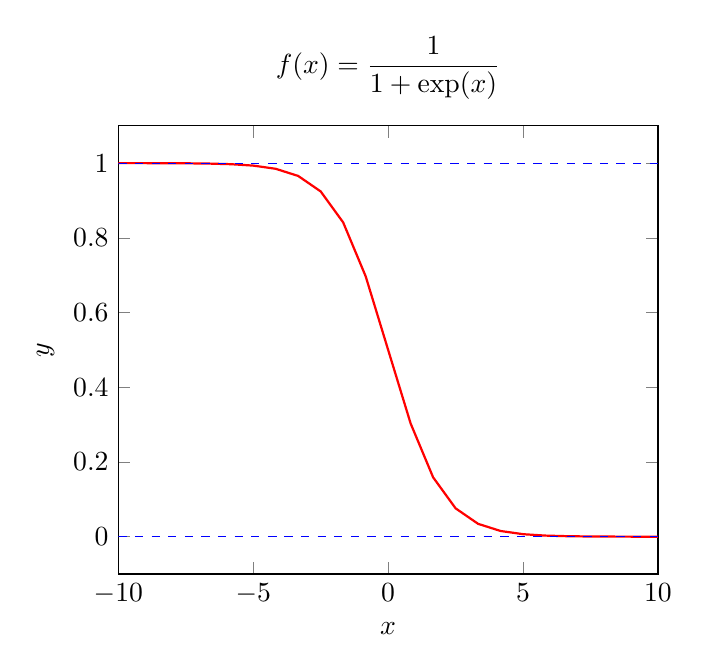
\begin{tikzpicture}
		\begin{axis}[
				title={$\dps{f(x) = \frac{1}{1 + \exp(x)}}$},
				xlabel={$x$},
				ylabel={$y$},
				xmin=-10, xmax=10,
				ymin=-0.1, ymax=1.1,
			]
			\addplot[color=red, thick, domain=-10:10] {1 / (1+exp(x))};
			\addplot[color=blue, dashed, domain=-10:10] {1};
			\addplot[color=blue, dashed, domain=-10:10] {0};
		\end{axis}
	\end{tikzpicture}
\end{center}
\subsection*{Comparing Cardinalities}
For two sets, $X$ and $Y$ 
\begin{itemize}
	\item $\abs{X}\leq\abs{Y}\iff \exists\ \text{injective}\ f:X\to Y$
	\item $\abs{X}\geq\abs{Y}\iff \exists\ \text{surrjective}\ f:X\to Y$
	\item $\abs{X}<\abs{Y}\iff \exists\ \text{injective and not surrjective}\ f:X\to Y$
	\item $\abs{X}>\abs{Y}\iff \exists\ \text{surrjective and not injective}\ f:X\to Y$
	\item $\abs{\emp} < \abs{X}$ and $\abs{X} > \abs{\emp}$ $\forall X\neq\emp$
\end{itemize}

\thm{Schr\"oder-Bernstein Theorem}{
	For two sets, $X,\ Y$,
	$$
		\abs{X}\leq\abs{Y},\ \abs{X}\geq\abs{Y}\implies \abs{X}=\abs{Y}
	$$
}
Therefore, to show that two sets have equal cardinality, it is enough to find
\begin{enumerate}
	\item an injective function, $f:X\to Y$ and
	\item a surrjective function, $f:X\to Y$
\end{enumerate}
Or
\begin{enumerate}
	\item an injective function, $f:X\to Y$ and
	\item an injective function, $f:Y\to X$ 
\end{enumerate}
Or
\begin{enumerate}
	\item a surrjective function, $f:X\to Y$ and
	\item a surrjective function, $f:Y\to X$ 
\end{enumerate}
This can be easier then finding a bijection between the two sets.

\section{Lecture 23}
\subsection*{Relations on Sets}
\dfn{Relation}{
	Given sets $A$ and $B$, a binary relation $\alpha$ from $A$ to $B$ is a subset of the Cartesian product of $A$ and $B$. If $(x,y)\in\alpha$ we can also write $x\mathbin{\alpha}y$, and we say $x$ is related to $y$.
}

\ex{}{
	Let $A=\braces{1,2,5}$ and $B=\braces{5,6}$, define a binary relation $\sigma$ by
	$$
		\forall a\in A,\ b\in B,\ a\mathbin{\sigma}b \iff a<b
	$$
	Then
	$$
		A\times B \supseteq \sigma = \braces{(1,5), (1,6), (2,5), (2,6), (5,6)}
	$$
}	
We can represent this with a diagram, drawing arrows from the elements in set $A$ to elements in set $B$. We draw an error if and only if the element in $A$ is related to the element in $B$. \\

We can thereby observe that a relation is a generalisation of a function.

\dfn{Inverse Relation}{
	If $\rho$ is a relation from sets $A$ to $B$, then the inverse relation $\rho\inv$ is defined by
	$$
		\rho\inv = \braces{(b,a)\in B\times A \suchthat (a,b) \in\rho}
	$$
}

\ex{}{
	Let $A=\braces{2,3}$ and $B=\braces{2,6,9}$ and $\rho\subseteq(A,B)$ such that
	$$
		\forall a\in A,\ b\in B,\ a \mathbin{\rho} b \iff a\divs b
	$$
	Then
	$$
		\rho = \braces{(2,2), (2,6), (3,6), (3,9)}
	$$
	and
	$$
		\rho\inv = \braces{(2,2), (6,2), (6,3), (9,3)}
	$$
}

\dfn{}{
	A relation on a set, is a realtion from a set $A$ to itself.
}

\ex{}{
	Let $\rho$ be a relation on set $A=\braces{2,3,6}$:
	$$
		\forall x,y\in A,\ x\mathbin{\rho}y \iff x \divs y
	$$
	Then
	$$
		A\times A \supseteq \rho = \braces{(2,2), (3,3), (6,6), (2,6), (3,6)}
	$$
}

\dfn{}{
	Let $\rho$ be a relation on a set $A$.
	\begin{itemize}
		\item $\rho$ is reflexive $\iff \forall x\in A,\ x\mathbin{\rho}x$
		\item $\rho$ is symmetric $\iff \forall x,y\in A,\ x\mathbin{\rho}y \implies y\mathbin{\rho}x$
		\item $\rho$ is transitive $\iff \forall x,y,z\in A,\ x\mathbin{\rho}y,\ y\mathbin{\rho}z \implies x\mathbin{\rho} z$	
	\end{itemize}
}

On an arrow diagram, a relation is
\begin{itemize}
	\item reflexive if and only if every element has an arrow pointing to itself.
	\item symmetric if and only if for every arrow from one element to another, there is a second arrow travelling in the opposite direction.
	\item transitive if and only if for every two consecutive arrows, there is a third arrow connecting the ultimate start element with the ultimate end location (think about how the opposite and adjacent lengths of a triangle connect points $P$ to $Q$ and $Q$ to $R$, but the hypotenuse ultimately connects $P$ to $R$.)
\end{itemize}

\ex{}{
	Let $d\in\bbn$ be fixed. The relation $\rho$ on $\bbz$, defined by
	$$
		\forall a,b\in\bbz,\ a\mathbin\rho b\iff a\equiv b\Mod d 
	$$
	\begin{gather*}
		\intertext{Is reflexive}
		\Suppose a\in\bbz \\ \Then a-a = 0 \\ d \divs 0 \iff a\equiv a\Mod d \\
		\tf a\mathbin\rho a
		\intertext{Is symmetric}
		\Suppose a,b\in\bbz,\ a\mathbin\rho b \\ \Then a\equiv b\Mod d,\ d\divs(a-b),\ d\divs -(b-a),\ d\divs(b-a) \iff b\equiv a\Mod d \\
		\tf b\mathbin\rho a
		\intertext{Is transitive}
		\Suppose a,b,c\in\bbz,\ a\mathbin\rho b,\ b\mathbin\rho c \\
		\Then a\equiv b\Mod d,\ b\equiv c\Mod d \\
		d \divs(a-b),\ d\divs(b-c) \iff d\divs(a-b)+(b-c) \iff d\divs(a-c) \iff a\equiv c\Mod d \\
		\tf a\mathbin\rho c
	\end{gather*}
}

\pagebreak
\Lemma A relation $\rho$ on set $A$ is symmetric if and only if $\rho=\rho\inv$.
\begin{proof}
	Let $\rho$ be a relation on set $A$. \\
	Show that $\rho$ is symmetric $\implies \rho=\rho\inv$
	\begin{list}{}{\rightmargin\leftmargin\topsep=4pt}\item
		Suppose $\rho$ is symmetric. 

		Let $(x,y)\in\rho$. Then $(y,x)\in\rho\inv$, because $\rho$ is symmetric. \\
		Hence, $(x,y)\in\rho\inv$. \\
		So, $\rho\subseteq\rho\inv$. 

		Now, let $(x,y)\in\rho\inv$. Then $(y,x)\in\rho$ by defintion. \\
		Hence $(x,y)\in\rho$, since $\rho\inv$ is symmetric. \\
		So, $\rho\inv\subseteqq\rho$.

		Therefore, $\rho=\rho\inv$
	\end{list}
	Show that $\rho=\rho\inv\implies\rho$ is symmetric.
	\begin{list}{}{\rightmargin\leftmargin\topsep=4pt}\item 
		Suppose $\rho=\rho\inv$

		Let $(x,y)\in\rho$. Then $(y,x)\in\rho\inv$. \\
		But, $\rho=\rho\inv$, therefore $(y,x)\in\rho$.

		Therefore, $\rho$ is symmetric.
	\end{list}
	Therefore, $\rho$ is symmetric $\iff\rho=\rho\inv$
\end{proof}

\chapter{Week 9}
\section{Lecture 24}
\subsection*{Equivalence Relations}
\dfn{Equivalence Relation}{
	Let $\rho$ be a relation on the set $A$. Then $\rho$ is an equivalence relation if and only if $\rho$ is symmetric, reflexive, and transitive.
}
\ex{}{
	The relation $\rho$ on $\bbz$ from example 8.2.4 is reflexive, symmetric and transitive.\\

	Therefore, $\rho$ is an equivalence relation.
}

\dfn{Equivalence Class}{
	Let $\rho$ be an equivalence relation on the set $A$, and let $a\in A$. \\

	The equivalence class of $a$ is 
	$$
		\sqbracks{a} = \braces{x\in A \suchthat x \rho a}
	$$
	So, $\forall x\in A,\ x\in\sqbracks{a}\iff x\mathbin{\rho} a$
}

\ex{}{
	Let $\rho$ be the relation on $\bbz$ defined by $a\mathbin{\rho} b \iff a\equiv b\Mod 3 \iff 3\divs(a-b)$. \\

	Then $\rho$ is an equivalence relation with equivalence classes
	$$
		\begin{array}{c}
			\sqbracks{0} = \braces{\dots,-6,-3,0,3,6,\dots} \\
			\sqbracks{1} = \braces{\dots,-5,-2,1,4,7,\dots} \\
			\sqbracks{2} = \braces{\dots,-4,-1,2,5,8,\dots} \\
		\end{array}
	$$
	Notice that $[0]=[3]=[-6]$, etc. \\
	Also notice that every element of the set has been put into one of these classes. A partition
}
\Lemma Let $\rho$ be an equivalence relation on $S$ and $a,b\in S: a\mathbin{\rho}b$, then $\sqbracks{a}=\sqbracks{b}$.
\begin{proof}
	Let $\rho$ be an equivalence relation on the set $A$, $a,b\in A$, and $a\mathbin\rho b$. \\
	Show $\sqbracks{a}\subseteq\sqbracks{b}$
	\begin{list}{}{\rightmargin\leftmargin\topsep=4pt}\item
		Let $x\in\sqbracks{a}$. Then $x\mathbin\rho a$, by defintion. \\
		Now, since $x\mathbin\rho a$ and $a\mathbin\rho b$, then $x\mathbin\rho b$, by the transitive property. \\
		Thus, $x\in\sqbracks{b}$

		$\tf\sqbracks{a}\subseteq\sqbracks{b}$
	\end{list}
	Show $\sqbracks{b}\subseteq\sqbracks{a}$
	\begin{list}{}{\rightmargin\leftmargin\topsep=4pt}\item
		Let $x\in\sqbracks{b}$. Then $x\mathbin\rho b$, by defintion. \\
		Now, since $x\mathbin\rho b$ and $b\mathbin\rho a$, then $x\mathbin\rho a$, by the transitive property. \\
		Thus, $x\in\sqbracks{a}$

		$\tf\sqbracks{b}\subseteq\sqbracks{a}$
	\end{list}
	$\tf \sqbracks{a}=\sqbracks{b}$
\end{proof}

\Lemma If $\rho$ is an equivalence relation on the set $A$, and $a,b\in A$ and $\sqbracks{A}\cap\sqbracks{B}\neq\emp$, then $\sqbracks{A}=\sqbracks{B}$.

Or, equivalently

If $\rho$ is an equivalence relation on the set $A$, and $a,b\in A$, then either $\sqbracks{A}\cap\sqbracks{B}\cap\emp$ or $\sqbracks{A}=\sqbracks{B}$.

\thm{}{
	If $\rho$ is an equivalence relation on $A$, then the set of equivalence classes of $\rho$ form a partition of $A$.

	$$
		\bigcup_{\forall a\in A} \sqbracks{a} = A
	$$
}

This can work in the opposite direction too, \\

\Theom Given a partition of $A$, and a binary relation $\rho$, induced by the parition, it follows that $\rho$ is reflexive, symmetric, and transitive.

\section{Lecture 25}
\subsection*{Partial Order Relations}
\dfn{Antisymmetric}{
	A relation $\rho$ on a set $A$ is antisymmetric if and only if
	$$
		\forall a,b\in A,\ a\mathbin\rho b,\ b\mathbin\rho a \implies a=b
	$$
}

\dfn{Partial Order Relation}{
	A relation $\rho$ on the set $A$ is a partial order relation on $A$ if an only if $\rho$ is reflexive, antisymmetric, and transitive.	
}

\ex{}{
	Consider the relation ``less than or equal to'' on $\bbr$
	\begin{itemize}
		\item Reflexive: $\forall x\in\bbr,\ x\leq x$.
		\item Antisymmetric: $\forall x,y\in\bbr,\ x\leq y,\ y\leq x\implies x=y$.
		\item Transitive: $\forall x,y,z\in\bbr,\ x\leq y,\ y\leq z\implies x\leq z$.
	\end{itemize}
	Therefore, $\leq$ is a partial order relation on $\bbr$
}

\dfn{Comparable Elements}{
	Let $\rho$ be a relation on a set $A$. Elements $a,b\in A$ are comparable if and only if $a\mathbin\rho b$ or $b\mathbin\rho a$. Otherwise, $a$ and $b$ are uncomparable.
}

\dfn{Total Order Relation}{
	Let $\rho$ be a relation on a set $A$. Then $\rho$ is a total order relation if and only if $\rho$ is a partial order relation such that all elements are comparable. \\

	That is, $\rho$ is a total order relation if and only if
	\begin{itemize}
		\item $\rho$ is reflexive,
		\item $\rho$ is antisymmetric,
		\item $\rho$ is transitive,
		\item $\forall a,b\in A,\ a\mathbin\rho b \lor b\mathbin\rho a$.
	\end{itemize}
}

\ex{}{
	Show that the relation $\rho$ be defined by $a\mathbin\rho b\iff a\divs b$ on the set $A=\braces{1,2,4,8,16}$. Show that this relation is a total order relation on the set $A$. \\

	\begin{list}{}{\rightmargin\leftmargin\topsep=0pt}\item
		$\forall a\in A, a\divs a$. \\
		Therefore $\rho$ is reflexive on $A$.

		Suppose $a,b\in A$ and $a\divs b$ and $b\divs a$. \\
		Then $b=ka$ and $a=lb$, for some $k,l\in\bbn$. \\
		Thus $b=klb \iff 1 = lb$. Therefore $a=b$. \\
		Therefore, $\rho$ is antisymmetric

		Suppose $a,b,c\in A$ and $a\divs b$ and $b\divs c$. \\
		Then $b = ka$ and $c = lb$, for some $k,l\in\bbn$. \\
		Thus $c = kla$ Therfore $a\divs c$. \\
		Therefore, $\rho$ is transitive.

		Therefore, $\rho$ is a partial order relation.

		Let $a,b\in A$. \\
		Then, $a=2^k,\ b=2^l$, for some $k,l\in\braces{0,1,2,3,4}$. \\
		Without loss of generality, assume $k\leq l$. \\
		Then $b=2^l = 2^{l-k}2^k$. \\
		Since $2^k\in\bbz$, we have $2^k\divs b$, hence $a\divs a$. \\
		Therefore, all the elements of $A$ are comparable. \\

		Therefore $\rho$ is a total order relation on $A$.
	\end{list}
}

\section{Lecture 26}
\subsection*{Groups}
\dfn{Group}{
	Let $G$ be a set, and let $*$ be a binary operation, $*:G\times G\to G$. We call $(G,*)$ group if and only if it has the following properties:
	\begin{itemize}
		\item \textbf{Closure}: $\forall g,h\in G,\ g*h\in G$.
		\item \textbf{Associative}: $\forall g,h,k\in G,\ (g*h)*k = g*(h*k)$.
		\item \textbf{Identity}: $\exists i\in G: \forall i\in G,\ i*g=g*i=e$.
		\item \textbf{Inverse}: $\forall g\in G,\ \exists g\inv\in G: g*g\inv=g\inv*g=i$.
	\end{itemize}
}

\ex{}{
	$(\bbz, +)$ is a group.
	\begin{gather*}
		+:\bbz\times\bbz\to\bbz,\ +:(a,b)\mapsto a+b,\ a+b\in\bbz,\ \forall a,b\in\bbz. \text{ Hence, $(\bbz,+)$ is closed since } \\
		(a+b)+c = a+(b+c),\ \forall a,b,c\in\bbz, \text{ hence, $(\bbz,+)$ is associative} \\
		0\in\bbz: \forall n\in\bbz,\ 0+a = a+0 = a. \text{ Hence, 0 is the identity.} \\
		\forall a\in\bbz,\ -a\in\bbz,\ a+(-a) = (-a)+a = 0. \text{ Hence, every element has an inverse.}
	\end{gather*}
	Therefore, $(\bbz,+)$ is a group.
}

\ex{}{
	Is $(\bbr,\cd)$ a group?
	\begin{gather*}
		\text{Closure?}\ \forall x,y\in\bbr, x\cd y\in\bbr.\ \text{YES} \\
		\text{Associative?}\ \forall x,y,z\in\bbr, (x\cd y)\cd z = x\cd(y\cd z).\ \text{YES} \\
		\text{Identity?}\ 1\in\bbr,\ \forall x\in\bbr,\ 1\cd x= x\cd1 = x.\ \text{YES} \\
		\text{Inverse?}\ \forall x\in\bbr,\ \text{take}\ y=\frac{1}{x}\in\bbr,\ x\cd y = y\cd x = 1.\ \text{yes..?}\ 
		\text{EXCEPT}\ 0\in\bbr,\ \frac{1}{0}\notin\bbr.\ \text{NO!}
	\end{gather*}
	Therefore $(\bbr,\cd)$ is not a group. However, it's interesting to note that $(\bbr\setminus\braces{0},\cd)$ IS a group!
}

These are examples of an infinite groups, since the sets $\bbz$ and $\bbr$ are infinite sets. \\

Let's consider the set $\bbz_n$ where $\bbz_n$ denotes the set of equivalence classes of the integers modulo $n$,
$$
	\bbz_n = \braces{[0],[1],[2],\dots,[n-1]}
$$
Next we'll define
$$
	\begin{array}{c}
		+:\bbz_n\times\bbz_n\to\bbz_n,\ [a]+[b]=[a+b] \\
		\cd:\bbz_n\times\bbz_n\to\bbz_n,\ [a]\cd[b]=[a\cd b]
	\end{array}
$$

\ex{}{
	Consider $(\bbz_3, +)$ \\

	We can make an ``addition table'' to represent this
	$$
		\begin{array}{c|ccc}
			+			& [0] & [1] & [2] \\ \hline
			{[0]} & [0] & [1] & [2] \\
			{[1]} & [1] & [2] & [0] \\
			{[2]} & [2] & [0] & [1] \\
		\end{array}
	$$
	\begin{itemize}
		\item Closure: YES. Every element inside the table is in the set $\bbz_3$
		\item Associative: YES. 
		\item Identity: YES, namely $[0]$.
		\item Inverse: YES, namely $[0]\inv=[0],\ [1]\inv=[2],\ [2]\inv=[1]$.
	\end{itemize}
	Therefore, $(\bbz_3,+)$ is a group. \\
}

\nt{
	Note that the above table is called a Cayley Table, an $n\times n$ array with rows and columns labeled by the $n$ elements. The entry in column $x$, row $y$ is $x*y$, where $*$ is the group opperation.
}

\dfn{Abelian}{
	A group $(G,*)$ is called Abelian if the operation $*$ is commutative, that is 
	$$
		\forall g,h\in G,\ g*h = h*g
	$$
	Otherwise, we call the group non-Abelian.
}

For $n\in\bbn$, the symmetric group $S_n$ consists of all bijections
$$
	f:X\to X\ \text{where}\ X = \braces{a\in\bbn\suchthat a\leq n}
$$
under the operation $\circ$, the composition of functions. \\

We should note that $S_n$ is non-Abelian for $n\geq3$.

\chapter{Week 10}
\section{Lecture 27}
\subsection*{Elementary Properties of Groups}
\thm{	Uniquie Identity Element}{
	Suppose $(G,*)$ has two unique identity elements, $e_1$ and $e_2$. We can now evaluate $e_1*e_2$ in two ways. \\

	Since $e_1$ is the identity, and $e_2\in G$, $e_1 * e_2 = e_1$.

	Since $e_2$ is the identity, and $e_1\in G$, $e_1 * e_2 = e_2$.

	Hence, $e_1 = e_2$, but this is a contradiction, since $e_1$ and $e_2$ are defined to be unique identity elements. \\

	Hence, $(G,*)$ has only one unique identity element. $\QED$
}

\thm{Every Element has an Inverse}{
	Suppose $(G,*)$ is a group and $g\in G$ has an two unique inverses $h_1,\ h_2\in G$. Let $e$ be the identity of $(G,*)$. \\

	Then, $(h_1*g)*h_2	= e*h_2 = h_2$.

	And, $h_1*(g*h_2) = h_1 * e = h_1$. 

	So, $h_1 = h_2$, but this is a contradiction, since $h_1$ and $h_2$ is defined to be unique inverses of $g$. \\

	Therefore, for the group $(G,*)$ every element $g\in G$ has one unique inverse. $\QED$
}

\dfn{Subgroup}{
	Let $(G,*)$ be a group, and let $H\subseteq G$. We say that $H$ is a subgroup of $G$ if $(H,*)$ itself is a group. \\

	That is, H is a subgroup of G if:
	\begin{itemize}
		\item Closure: $\forall g,h\in H$, we have $g*h\in H$.
		\item Identity: $e$ is the identity of $(G,*)$, then $e\in H$.
		\item Inverses: $\forall h \in H,\ \exists h\inv: h*h\inv = e$.
	\end{itemize} 
	We write $H\leq G$ to denote ``$H$ is a subgroup of $G$'', when the group context is clear. \\

	If $H\leq G$ and $H\neq G$, then $H$ is a proper subgroup of $G$. \\

	If $e$ is the identity element of group $G$, then $(\braces{e},*)$ is a trivial subgroup.
}

\dfn{Element Powers}{
	Let $(G,*)$ be a group. By associativity we have $(a*b)*c = a*(b*c),\ \forall a,b,c\in G$. Thus, we can write $a*b*c$ without ambiguity. \\

	Given this group, and element $g\in G$, we can define powers as follows:
	\begin{itemize}
		\item $g^k = g*g*\dots*g\ (k\ \text{times}),\ k\in\bbz_+$.
		\item $g^{-k} = g\inv * g\inv * \dots * g\inv,\ (k\ \text{times}),\ k\in\bbz_+$.
		\item $g^0 = e$.
	\end{itemize}
}

\dfn{Cyclic Subgroups}{
	Let $a\in G$ be an element of the group $(G,*)$. We let $\brangle{a}$ denote ``the set generated by $a$,''
	$$
		\brangle{a} = \braces{a^k\suchthat k\in\bbz} = \braces{\dots, a^{-2}, a^{-1}, a^0, a^1, a^2, \dots}
	$$
	For any $a\in G$ where $(G,*)$ is a group, $\brangle{a}$ is a subgroup of $G$:
	\begin{itemize}
		\item Closure: $x,y\in\brangle{a},\ x=a^i,\ y=a^j,\ i,g\in\bbz$. Then, $x*y = a^i * a^j = a*(i+j)\in\brangle{a}$.
		\item Identity: $e = a^0\in\brangle{a}$. 
		\item Inverses: $x\inv = \braces{a^i}\inv = a^{-i} \in \brangle{a}$.
	\end{itemize}
	$\brangle{a}$ is called the cyclic subgroup of $G$ generated by $a$. \\

	If $G=\brangle{a}$ for some $a\in G$, we say $G$ is cyclic and $a$ is a generator of $G$.
}

\section{Lecture 28}
\subsection*{Group Isomorphisms}
\dfn{Isomorphic Groups}{
	Two groups, $(G,*)$ and $(H,\circ)$ are iosmorphic if and only if there exists a bijection $f:G\to H$ such that for all $x,y\in G$, $f(x*y) = f(x)\circ f(y)$. Such a bijection is called an isomorphism. \\

	If $f$ is an isomorphism from group $G$ to group $H$ and $e\in G$ and $\iota\in H$ are the identitiy elements of $G$ and $H$, respectively, then $f(e)=\iota$. \\

	If $G$ and $H$ are Isomorphic, they they share the same properties, like number of elements, abelian-ness, number of sub-groups, fundamental structure, etc.
}

\thm{}{
	For any prime $p$, the group $(\bbz_{p}\setminus\braces{0},\cd)$ is Isomorphic to $(\bbz_{p-1}, +)$, where $\bbz_n$ denotes the natural numbers modulo $n$.
}

\thm{}{
	Suppose $n,m\in\bbz_+$. Then $(\bbz_n\times\bbz_m,+)$ is Isomorphic to $(\bbz_{nm},+)$ if and only if $\gcd(n,m)=1$, (i.e. $n$ and $m$ are coprimee). \\

	This means that modular arithmetic for large numbers,
	$$
		n = p_1^{e_1}p_2^{e_2}p_3^{e_3}\dots p_n^{e_n}
	$$
	can be done with as arithmetic modulo the prime powers $p_i^{e_i}$.
}
Group isomorphism is important, because what we know about a groups, we also know about its Isomorphic groups.

\section{Lecture 29}
\subsection*{Fields}
\dfn{Field}{
	A field, $(F,+,\cd)$ consists of a set $F$, and two binary operators:
	\begin{itemize}
		\item $+:F\times F\to F$
		\item $\cd:F\times F\to F$
	\end{itemize}
	such that
	\begin{enumerate}
		\item $(F,+)$ is an Abelian group, with identity, $e$.
		\item $(F\setminus\braces{e}, \cd)$ is an Abelian group.
		\item $\forall f,g,h \in F,\ f\cd(g+h) = (f\cd g) + (f\cd h)$
		\item $\forall f,g,h \in F,\ (f+g)\cd h = (f\cd h) + (g\cd h)$
	\end{enumerate}
}
Consequently, a field will have two identities, an addative identity and a multiplicative identity. We will also have two types of inverses, addative inverses and multiplicative inverses. \\

Fields are used when defining structures in linear algebra, for example, the components of a vector or matricies can be elements of a field $(F,+,\cd)$. \\

Finite groups like $(\bbz_p, +, \cd)$ are important in computer science, because they can can ``behave'' like real numbers, but are small enough to describe precisely using finite bits.

\chapter{Week 11}
\section{Lecture 30}
\subsection*{Introduction to Counting}
\ex{}{
	Suppose a resturant has 5 types of cake and 2 types of ice cream. \\

	How many choices for dessert are there, if we select one cake, and one ice cream?
	$$
		5 \text{ cakes} \cd 2\text{ ice creams} = 10 \text{ choices}
	$$

	How many choices for dessert are there if we select either one cake or one ice cream?
	$$
		5 \text{ cakes} + 2 \text{ ice creams} = 7\text{ choices}
	$$

	In one example, we had a sequence of two separate \textbf{tasks}, and therefore, used a multiplication to find the answer. In the second, we only had one task, but were choosing from 2 types of options, and therefore addition was used to find the total.
}

\ex{}{
	Consier the set of all passwords consisting of 3 letters from the set $\braces{A, B, C, \dots, X, Y, Z}. $ \\

	How many passwords are possible?\\
	There are 26 choices for the first, second, and third letters.
	$$
		26\cd26\cd26 = 26^3 = 17.576\text{ passwords}
	$$

	How many passwords contain no repeated letters?
	There are 26 choices for the first letter, 25 for the second, and 24 for the third.
	$$
		26\cd25\cd24 = 15.600\text{ passwords with no repeated letters}
	$$

	How many passwords contain only vowels or only consonants? \\
	Here we need to consider and compute two options, then add them together. \\
	Option 1: only vowels
	$$
		5\cd5\cd5 = 5^3 = 125
	$$
	Option 2: only consonants
	$$
		21\cd21\cd21 = 21^3 = 9.261
	$$
	Total = option 1 + option 2
	$$
		5^3 + 21^3 = 9.386
	$$
}

\dfn{Permutation}{
	A permutation of a set of objects is an arrangement of the objects into an order. \\

	\Theom A set with cardinality $n$ elements will have $n!$ permutations.
}

\ex{}{
	Consider the permutations of the letters of the word OBJECTS. \\

	How many start with a vowel? \\
	Option 1: words starting with O
	$$
		1\text{ choice for first letter (O)}\cd 6\cd5\cd4\cd3\cd2\cd1 \text{ choices for proceeding letters} = 6! = 720
	$$
	Option 2: words starting with E
	$$
		1\text{ choice for first letter (E)}\cd 6\cd5\cd4\cd3\cd2\cd1 \text{ choices for proceeding letters} = 6! = 720
	$$
	Total = option 1 + option 2
	$$
		6! + 6! = 720+720 = 1440
	$$

	\textbf{Alternatively} (and more elegantly) we can calculate it in one go, by noting that we have two choices for the first letter,
	$$
		1\text{ choices for first letter (O/E)}\cd 6\cd5\cd4\cd3\cd2\cd1 \text{ choices for proceeding letters} = 2\cd 6! = 1440
	$$
}

\ex{}{
	Consider all license plates consisting of 3 letters from the set $\braces{A,B,\dots,Y,Z}$ followed by 3 digits from the set $\braces{0,1,\dots,8,9}$. \\
	
	How many plates are possible?
	$$
		10\cd10\cd10\cd26\cd26\cd26 = 10^3\cd26^3 = 17.576.000
	$$
	How many plates have no repeated symbols (digits or letters)?
	$$
		10\cd9\cd8\cd26\cd25\cd24 = 11.232.000
	$$
	How many plates have at least one repeated symbol?\\
	We note that we've already calcualted the total number of plates, and the number of plates with no repeated digits. Therefore the number of plates with at least one repeated digit will be the total minus the number without repeated digits
	$$
		17.576.000 - 11.232.000 = 6.344.000
	$$
}

\section{Lecture 31}
\subsection*{Counting Selections}
Let $n$ and $r$ be nonnegative integers. \\

\textbf{Problem}:\\
Select $r$ elements from a set of $n$ elements. How many ways are there to make the selections? \\

Considerations:
\begin{itemize}
	\item Does order matter?
	\item Is repition of element selections allowed?
\end{itemize}

\subsubsection*{Order matters, Repititions allowed}
\ex{}{
	Suppose we need to choose a PIN number, and we may do so from the set
	$$
		S = \braces{0,1,2,3,4,5,6,7,8,9}
	$$
	Order matters, and we may choose the same digit multiple times. How many PINs are there? \\

	In each of 4 selections, we have 10 choices, hence
	$$
		\text{total} = 10\cd10\cd10\cd10 = 10^4 = 10.000\text{ possibilities}
	$$
}
\Theom In general, the number of selections of $r$ elements from a set containing $n$ elements, where order matters and repition is allowed is
$$
	T(n,r) = n^r
$$
	
\subsubsection*{Order matter, Repitions disallowed}
\ex{}{
	If there are 7 runners in race, in how many ways can First, Second, and Third place be awarded? \\
	There are 7 runners which can possibly come first. This runner is removed form the pool, hence there are 6 possible runners who can come second. That runner is removed from the pool, and finally, there are 5 possible runners who can come third.
	$$
		\text{total} = 7\cd6\cd5 = 210 \text{ possible podiums}
	$$
}
\Defin{$r$-permutation} Let $n$ and $r$ be nonnegative integers, with $r\leq n$. An $r$-permutation of a set is an ordered selection of $r$ elements taken from the set of $n$ elements. The total number of possible $r$-permutations is denoted $\perm{n}{r}$. \\

So, in the previous example, we calcualted $\perm{7}{3}$. 

\thm{$\perm{n}{r}$}{
	If $n,r\in\bbz$ and $1\leq r \leq n$, then
	$$
		\perm{n}{r} = n(n-1)(n-2)\dots(n-r+1) = \frac{n!}{(n-r)!}
	$$
}

\subsubsection*{Order does not matter, Repitions disallowed}
\ex{}{
	In how many ways can we select a 5 student commitee from a class of 15 students? \\
	If order mattered, we would count
	$$
		\perm{15}{5} = \frac{15!}{10!} = 15\cd14\cd13\cd12\cd11 = 360.360
	$$
	However, order does matter, and we've overcounted. Because commitee $ABCDE$ is the same as commitee $ECDBA$. In fact each set of 5 students has been overcounted $5!=120$ times, one for each ordering. So the actual number of commitees we could form is
	$$
		\frac{\perm{15}{5}}{5!} = \frac{15!}{5!10!} = \frac{360.360}{120} = 3.003
	$$
	Overcounting is generally fine, as long as we keep track by how much we've overcounted, to find the true answer in the end.
}	

\Defin{$r$-combination} Let $n,r$ be nonnegative integers, with $r\leq n$. An $r$-combination of a set of $n$ elements is a subset of $r$ of the $n$ elements. The total number of $r$-combinations of a set can be denoted $\mathrm{C}(n,r)$, which is consistent with the permutation's notation, however $\comb{n}{r}$ is more common and is read ``$n$ choose $r$.''

\thm{$\comb{n}{r}$}{
	If $n,r\in\bbz$ with $0\leq r\leq n$ then
	$$
		\comb{n}{r} = \frac{\perm{n}{r}}{r!} = \frac{n!}{r!(n-r)!}
	$$
}

\subsubsection*{Order does not matter, Repition is allowed}
\ex{}{
	Suppose a store has 4 large buckets of each with a different type of candy: red, yellow, blue, and pink. If you select a total of 7 candies, how many different choices are possible? \\

	Select 7 elements from $\braces{r,b,y,p}$ (repition is allowed) and order doesn't matter, for example $rrbbypp$ is the same as $rbrbpyp$. \\

	The answer is 120
}

We will not give a generalised solution to this problem in this class. \\

I however did some research, and found that this is known in combinatorics as ``combinations with repitions'' or multisets. The formula is 
$$
	\multiset{n}{r} = \comb{n+r-1}{r} = \frac{(n+r-1)!}{r!(n-1)!}
$$
and can be read ``$n$ multichoose $r$.'' This type of problem typically requires a bit more background in combinatorial reasoning. A further combinatorics course will certainly cover this topic.

\subsubsection*{Permutations of Typed objects}
\ex{}{
	How many permutations of the letters ``$AAAFFLL$'' are there? \\

	Method 1: There are 7 possible positions. We can place the $A$s in 3 of the 7 positions, the $F$s in 2 of the \underline{remaining} 4 positions, and the 2 $L$s in the remaining 2 positions.
	$$
		\comb{7}{3} \cd \comb{4}{2} \cd \comb{2}{2} = \frac{7!}{3!4!} \cd \frac{4!}{2!2!} \cd \frac{2!}{2!0!} = 35\cd 6\cd 1 = 210
	$$
	Note that, we could have also placed the $L$s then the $F$s then the $A$s, or any other order. The total comes out the same. Showing this is left as an exercise to the reader. \\

	Method 2: We could treat the letters as distinguishable, for example, $A_1A_2A_3F_1F_2L_1L_2$. Then the total number of orderings is simply
	$$
		\perm{7}{7} = \frac{7!}{0!} = 7! = 5.040
	$$
	However, we've now overcounted by some factor. $A_1A_2A_3F_1F_2L_1L_2$ is counted as a different solutions as $A_3A_2A_1F_2F_1L_2L_1$. In fact, the $A$s have been overcounted by a factor of $3!$ (one for each ordering of $A$s). Similarly, the $F$s and $L$s have been overcounted by factors of $2!$. Therfore, we need to divide through by these overcounting factors.
	$$
		\frac{5.040}{3!2!2!} = \frac{5.040}{6\cd2\cd2} = 210
	$$
}
\thm{Numbr Permutations of Typed Elements}{
	Suppose we have $n$ objects of which $n_1$ is type 1, $n_2$ is type 2\dots $n_k$ is type $k$. The number of distinct permutations of the $n$ objects is
	$$
		\comb{n}{n_1}\cd\comb{n-n_1}{n_2}\cd\dots\cd\comb{n-n_1-n_2-\dots-n_k}{k} = \frac{n!}{n_1!n_2!\dots n_k!}
	$$
}

Note that, the LHS of Theorem 11.2.3 corresponds to method 1 Example 11.2.5, whereas the RHS corresponds to method 2.

\chapter{Week 12}
\section{Lecture 32}
\subsection*{Probability}
\ex{}{
	Let's flip 2 fair coins. \\
	
	What is the probability that both coins land heads up? \\
	There are 4 possabilities:
	$$
		HH \qquad HT \qquad TH \qquad TT
	$$
	and each outcome is equally likely. Therefore, the probability of $HH$ occuring is 1 in 4, or 25\%. \\

	What is the probability of at least one coin landing face up? \\
	The outcomes with at least one $T$ are $HT$, $TH$, $TT$, which is 3 in 4, or 75\%.
}

\Defin{Random Procees} A process is said to be random if, when it takes place, one outcome from some set of possible outcomes occurs, but it is impossible to predict with certianty which outcome it will be. \\

\Defin{Sample Space} A sample space is the set of all possible outcomes of a random process of an experiment. \\

For example, in our example above, the sample space was
$$
	S = \braces{HH, HT, TH, TT}.
$$

\Defin{Event} An event is a subset of the sample space. \\

In the above example, we examined two events,
$$
	E_1 = {HH},\qquad E_2 = {HT, TH, TT}.
$$

\dfn{Finite Probability with Uniform Likelihood}{
	If $S$ is a finite sample space in which all outcomes are equally likely to occur, and $E$ is an event in $S$, then the probability of $E$, denoted $\prob{E}$ is
	$$
		\prob{E} = \frac{\abs{E}}{\abs{S}}
	$$
}

\thm{Value of $\prob{E}$}{
	For any event $E$ in a finite sample sapce $S$, with uniform likelyhood across all elements of $S$ is
	$$
		0 \leq \prob{E} \leq 1
	$$
}

\ex{}{
	A fair coin is tossed 7 times. The sample space $S$ is the set of all sequences $H/T$ of length 7. $\tf \abs{S} = 2^7$. \\

	What is the probability that we get exactly 5 heads? \\
	$$
		\abs{E} = \comb{7}{5} \cd \comb{2}{2} = 21\qquad \tf\prob{E} = \frac{\abs{E}}{\abs{S}} = \frac{2^7}{21} \approx 0.1641
	$$

	What is the probability that we get at least 5 heads? \\
	The probability of getting at least 5 heads is equal to the probability of getting exactly 7 heads, plus exactly 6 heads plus exactly 5 heads.
	$$
		\abs{E} = \comb{7}{5}{\cd}\comb{2}{2} + \comb{7}{6}{\cd}\comb{1}{1} + \comb{7}{7}{\cd}\comb{0}{0} = 29\qquad \tf\prob{E} = \frac{29}{2^7} \approx 0.2266
	$$
}

\ex{}{
	A standard deck of cards consists of 52 cards, divided among 4 suits (spades, hearts, clubs, diamonds), with 13 cards each (2,3,4,5,6,7,8,9,10,J,Q,K,A). \\

	Suppose 3 cards are drawn at random from a deck. What is the probability that all 3 cards have the same suit?\\
	The sample space is the set of all possible selections of 3 cards from the deck of 52. Order does not matter, but repitition is not allowed.
	$$
		\abs{S} = \comb{52}{3} = 22.100
	$$
	Let $E$ be the set of 3 card selections that are all the same suit. This will consist of 2 tasks: (1) select a suit, (2) select 3 cards from it.
	$$
		\abs{E} = \comb{4}{1}\text{suits}\cd \comb{13}{3}\text{cards} = 4\cd286 = 1.144
	$$
	Therfore the probability of drawing 3 cards of the same suit is
	$$
		\prob{E} = \frac{\abs{E}}{\abs{S}} = \frac{1.114}{22.100} \approx 0.0504
	$$
}

\ex{}{
	Suppose there are 23 people in a room. What is the probability that there are at least two people who share a birthday? (Assuming 365 days a year, ignoring leap years.) \\

	The sample space is the set of all possible ordered lists of birthdays for the 23 people.
	$$
		\abs{S} = 365^23
	$$
	Let $E$ be the event that at least two people share a birthday. Let $E'$ be the event that all 23 people have different birthdays
	\begin{gather*}
		\abs{E'} = \perm{365}{23} = \frac{365!}{23!} \\
		\abs{E} = \abs{S} - \abs{E'}
	\end{gather*}
	So the probability of $E$ is
	$$
		\prob{E} = \frac{\abs{S} - \abs{E'}}{\abs{S}} = 1 - \frac{\abs{E'}}{\abs{S}} \approx 0.5073
	$$
	This is cool! The probability that two people share a birthday in only 23 people is greater then 50\%. 
}

\subsection*{Binomial Coefficients}
Let $n,r\in\bbz$ and $0\leq r \leq n$. Let $S$ be a set with with $\abs{S}=n$.
$$
	\comb{n}{r} = \genfrac{}{}{0pt}{}{\text{\# of subsets of with } S}{\text{exatly } r \text{ elements}} = \frac{n!}{r!(n-r)!}
$$
The result is called a binomial coefficient. \\

\Claim $\comb{n}{r} = \comb{n}{n-r}$ \\
\Proof
$$
	\comb{n}{n-r} = \frac{n!}{(n-r)!(n-(n-r)!)} = \frac{n!}{(n-r!)(r!)} = \frac{n!}{r!(n-r)!} = \comb{n}{r}
$$
$\QED$ \\

\thm{Pascal's Formula}{
	Let $n,r\in\bbz$ and $l\leq r\leq n$. Then
	$$
		\comb{n+1}{r} = \comb{n}{r-1} + \comb{n}{r}
	$$
	
	\proof By algebra.
	\begin{align*}
		\comb{n}{r-1} + \comb{n}{r} &= \frac{n!}{(r-1)!(n-r+1)!} + \frac{n!}{r!(n-r)!} \\
			&= \frac{n!}{(r-1)!(n-r+1)!}\cd\frac{r}{r} + \frac{n!}{r!(n-r)!}\frac{n-r+1}{n-r+1} \\
			&= \frac{r\cd n!}{r!(n-r+1)!} + \frac{n!(n-r+1)}{r!(n-r+1)!} \\
			&= \frac{r\cd n! + n!(n-r+1)}{r!(n-r+1)!} \\
			&= \frac{r\cd n! + n\cd n! - r\cd n! + n!}{r!(n-r+1)!} \\
			&= \frac{n!(n+1)}{r!(n-r+1)!} \\
			&= \frac{(n+1)!}{r!(n+1-r)!} \\
			&= \comb{n+1}{r} \tag*{\qed}
	\end{align*}

	\proof By combinatorics. \\
	Let $S$ be a set with cardinality $\abs{S} = n+1$. Then $\comb{n+1}{r}$ is the number of ways of choosing $A\subseteq S$ with $\abs{A} = r$. \\
	
	Fix a particular $x\in S$. The number of $r$-subsets of $S$ is the number of that contain $x$ plus the number that do not contain $x$.
	\begin{enumerate}
		\item The number of subsets $A\subseteq S$ with $\abs{A}=r$ and $x\in A$ is $\comb{n}{r-1}$.
		\item The number of subsets $A\subseteq S$ with $\abs{A}=r$ and $x\notin A$ is $\comb{n}{r}$.
	\end{enumerate}
	Therefore,
	\begin{equation*}
		\comb{n+1}{r} = \comb{n}{r-1} + \comb{n}{r} \tag*{\qed}
	\end{equation*}
}

\thm{Binomial Theorem}{
	Given any real numbers $a,b$ and any nonnegative integer $n$,
	\begin{align*}
		(a+b)^n	&= \sum_{k=0}^{n} \comb{n}{k}a^{n-k}b^k \\
			&= a^n + \comb{n}{1}a^{n-1}b^1 + \comb{n}{2}a^{n-2}b^2 + \dots + \comb{n}{n-2} a^{2}b^{n-2} + \comb{n}{n-1}a^1b^{n-1} + b^n		
	\end{align*}

	\begin{proof}
		If $n=0$, we have $(a+b)^0=1$ and 
		$$
			\sum_{k=0}^{0} \comb{0}{k}a^{0-k}b^k = \comb{0}{0}a^0b^0 = \comb{0}{0} = \frac{0!}{0!(0-0)!} = 1.
		$$
		So the theorem holds for $n=0$. \\

		For $n\geq 1$ we present a combinatorial proof. Let's consider small $n$s,
		\begin{gather*}
			(a+b)^2 = (a+b)(a+b) = a^2 + 2ab + b^2 \\
			(a+b)^3 = (a+b)(a+b)(a+b) = a^3 + 3a^2b + 3ab^2 + b^3
		\end{gather*}
		Expanding $(a+b)^k$ gives us the sum of all ordered combinations of $n$ symbols, each of which is $a$ or $b$. \\
		For each $k=0,1,2\dots n,$ 
		$$
			a^{n-k}b^k = \underbrace{a\cd a\cd a\cd \dots\cd a}_{n-k}\cd\underbrace{b\cd b\cd b\cd \dots \cd b}_{k}
		$$
		occurs exactly $\comb{n}{k}$ times in the expansion of $(a+b)^n$ since there are $\comb{n}{k}$ ways to choose the position of the $b$s and the $a$s fill the remaining posisions.\\
		$$
			\tf (a+b)^k = \sum_{k=0}^{n}\comb{n}{k}a^{n-k}b^k
		$$
	\end{proof}
}

\ex{}{
	Expand $(x+y)^4$ using the binomial theorem.
	\begin{align*}
		(x+y)^4 &= \sum_{k=0}^{4}\comb{4}{k}a^{4-k}b^k \\
			&= \comb{4}{0}a^{4-0}b^{0} + \comb{4}{1}a^{4-1}b^{1} + \comb{4}{2}a^{4-2}b^{2} + \comb{4}{3}a^{4-3}b^{3} + \comb{4}{4}a^{4-4}b^{4} \\
			&= 1a^4b^0 + 4a^3b^1 + 6a^2b^2 + 4a^1b^3 + 1a^0b^4 \\
			&= a^4 + 4a^3b + 6a^2b^2 + 4a^1b^3 + b^4 
	\end{align*}

	What is the coefficient of $x^5$ in the expanded form of $(x-1)^8$? \\
	$$
		(x-1)^8 = \sum_{k=0}^{8}\comb{8}{k} x^{n-k}(-1)^k
	$$
	$x^5$ occurs when $k=8-5=3$, so the binomial coefficient is
	$$
		\comb{8}{3}(-1)^{3} = 56\cd-1 = -56
	$$
}

\section{Lecture 33}
\subsection*{The Inclusion-Exclusion Principle}
\ex{}{
	Suppose in a fishtank there are 14 blue fish, 7 striped fish, and 4 fish which are blue \textit{and} striped. How many fish are blue \textit{and} striped? \\

	If we add the blue fish and the striped fish, we get $14+7=21$. However, we've double counted the blue striped which are included in both groups. To get around this, we substract the fish which are blue \textit{or} striped, and the actual answer is
	$$
		\abs{\text{blue and striped}} = \abs{\text{blue}} + \abs{\text{striped}} - \abs{\text{blue or striped}} = 14 + 7 - 4 = 17
	$$
}

\thm{The Inclusion-Exclusion Principle for Two Sets}{
	For any two sets, $A$ and $B$,
	$$
		\abs{A\cup B} = \abs{A} + \abs{B} - \abs{A\cap B}
	$$

	A special case of the theorem is for two \textbf{disjoint} sets $A$ and $B$, so $\abs{A\cap B}=0$. Therefore, $\abs{A\cup B} = \abs{A} + \abs{B}$.
}

\ex{}{
	Suppose $A,B$ are sets with $\abs{A}=9,\ \abs{B}=15,\ \abs{A\cup B}=19$. What is $\abs{A\cap B}$?
	$$
		\abs{A\cup B} = \abs{A} + \abs{B} - \abs{A\cap B} \iff 19 = 9 + 15 - \abs{A\cap B} \iff \abs{A\cap B} = 9 + 15 - 19 = 24 - 19 = 5
	$$
}

\thm{The Inclusion-Exclusion Principle for Three Sets}{
	For any three sets, $A,\ B,\ C$,
	\begin{align*}
		\abs{A\cup B\cup C} &= \phantom{-} \abs{A} + \abs{B} + \abs{C} \\
			&\phantom{=} - \abs{A\cap B} - \abs{A\cap C} - \abs{B\cap C} \\
			&\phantom{=} + \abs{A\cap B\cap C} 
	\end{align*}
}

\ex{}{
	100 students are surveyed about the subjects they are taking. \\
	\begin{tabular}{rl}
		50 & students are taking maths \\
		40 & students are taking chemistry \\
		35 & students are taking physics \\
		18 & students are taking maths and chemistry \\
		15 & students are taking maths and physics \\
		16 & students are taking chemistry and physics \\
		10 & students are taking all 3 subjects \\
	\end{tabular}
	How many students are taking none of the subjects? \\

	Let M, C, P denote the sets of students only taking maths, chemistry, or physics, respectively.
	\begin{align*}
		\abs{M\cup C\cup P} &= \abs{M} + \abs{C} + \abs{P} - \abs{M\cap C} - \abs{M\cap P} - \abs{C\cap P} + \abs{M\cap C\cap P} \\
			&= 50 + 40 + 35 - 18 - 15 - 16 + 10 \\
			&= 86 \\
		\tf\abs{(M\cup C\cup P)'} = 14
	\end{align*}
	So 14 students take none of the subjects maths, chemistry, or physics.
}

\section{Lecture 34}
\dfn{The Pigeonhole Principle}{
	Suppose you have $n$ pigeons sitting in $k$ pigeonholes. If $n>k$, then at least one pigeonhole contains two pigeons. \vspace{3pt} 

	If a function maps from a finite set to a finite set with smaller cardinality, then it cannot be injective. \\
	
	The contrapositive of the pigeonhole principle is: If you have $n$ pigeons sitting in $k$ pigeonholes, if each pigeonhole contains at most one pigeon, then $n\leq k$. \vspace{3pt}

	If a function is injective, then it maps from a finite set to a set with equal or greater cardinality.
}

\ex{}{
	If you have socks of 3 different colours in your drawer, what is the minimum number of socks you need to pull out in order to guarantee a matching pair?
	$$
		\text{pigeons}=\text{socks}\qquad \text{pigeonholes}=\text{colours}
	$$
	Since $\#\text{colors}=3$, $\#\text{socks}=4>3$.

	Suppose there are 680 people in a room. Must there be at least two people with the exact same initals?
	$$
		\text{pigeons}=\text{people}\qquad \text{pigeonholes}=\text{initals}
	$$
	Since $\#\text{initals}=26\cd26=676$ and $680 > 676$, then yes, at least two people share initals. \\

	Suppose $n\in\bbz_+$ and $n\geq 3$. Show that in every group of $n$ people there are at least two people who have the same number of friends within the group. 
	$$
		\text{pigeons}=\text{people}\qquad \text{pigeonholes}=\text{friends}
	$$
	Let $f:\bbz_{\geq3}\to\bbz_{+}$ map the $i$th person, $p_i$, to the number of friends $p_i$ has. Let $f(p_1)=1,\ f(p_2)=2, \dots, f(p_{n-1}) = n-1$. Now, $f(p_n)$ needs to map to something. All of the integers before it have been mapped to, and $p_n\not\mapsto n$ because a person cannot be friends with themselves. Therefore, by the pigeonhole principle, at least two people must have the same number of friends.
}

\thm{Generalised Pigeonhole Principle}{
	Suppose you have $n$ pigeons sitting in $k$ pigeonholes. If $n > km$, then at least one of the pigeonholes contains at least $m+1$ pigeons. \\

	The contrapositve form: Suppose you have $n$ pigeons sitting in $k$ pigeonholes. If each pigeonhole contains at most $m$ pigeons then $n\leq km$.
}

\ex{}{
	Show that in a group of 25 people, at least 3 people share a birthmonth.

	$$
		n=25,\quad m=2,\quad k=12,\quad n=25 > 24 = 12\cd 2 = k\cd m
	$$
	By the generalised pigeonhole principle, at least 3 people share a birthmonth.
}

\chapter{Week 13}
\section{Lecture 35}
\subsection*{Introduction to Graph Theory}
\begin{center}
	\tikz\graph[multi, clockwise=3]{
		a ->[out=110, in=70, looseness=8] a;
		b ->[out=335, in=295, looseness=8] b;
		c ->[out=245, in=205, looseness=8] c;
		a <-> b;
		a <-> c;
		b <-> c;
	};
\end{center}

\dfn{Graph}{
	A graph, $G$, consists of two finite sets:
	\begin{itemize}
		\item a nonempty set of vertices, $V(G)$.
		\item a possibly empty set of edges, $E(G)$, where each edge is associated with a set $\braces{v,w}\subseteq V(G)$. \\ The vertices $v$ and $w$ are called the endpoints of the edge.
	\end{itemize}
}
\ex{}{
	\begin{center}
		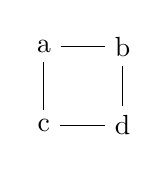
\begin{tikzpicture}[baseline={(current bounding box.center)}]
			\graph[grid placement] {[n=4, wrap after=2]
				a -- b -- a -- c -- d -- b;
			};
		\end{tikzpicture} \hspace{1cm}
		\begin{tikzpicture}[baseline={(current bounding box.center)}]
			\graph[multi, grow right]{
				a -- b -- c -- d;
				a --[out=45, in=225, looseness=1.5] d;
			};
		\end{tikzpicture}
	\end{center}

	This graph $G$ has $V(G) = \braces{a,b,c,d}$ and $E(G)=\braces{\braces{a,b}, \braces{b,c}, \braces{c,d}, \braces{a,d}}$. \\

	Note that both these representations are equivalent. How the graph is drawn is irrelevent, what matters is the relationships between vertices and edges.
}

\dfn{Loops, Parallel Edges, Simple Graphs}{
	\begin{center}
		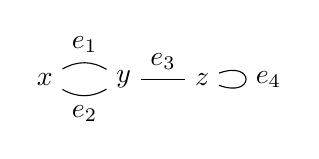
\begin{tikzpicture}[baseline={(current bounding box.center)}]
			\graph[multi, grow right]{
				x/$x$ --["$e_1$", bend left] y/$y$ --["$e_3$"] z/$z$ --["$e_4$" right, out=-20, in=20, looseness=8] z;
				x --["$e_2$" below, bend right] y;
			};
		\end{tikzpicture}
		$$
			V(G) = \braces{x,y,z}\qquad E(G) = \braces{e_1, e_2, e_3, e_4}
		$$
	\end{center}
	\Defin{Loop} A loops is an edge whose endpoints are equal, which is denoted $\braces{v,v}$ or $\braces{v}$. \\
	\Defin{Parallel Edges} Edges are parallel (also called multiple edges) if their is at least one other edge with the same set of endpoints. \\
	\Defin{Simple Graph} A simele graph is a graph with no loops or parallel edges. \\

	The example above has a loop, $e_4$, has a pair of parallel edges, $e_1,e_2$, and is therefore not a simple graph
}

\ex{}{
	\begin{center}
		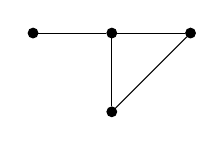
\begin{tikzpicture}[baseline={(current bounding box.center)}]
			\graph[no placement, nodes={circle, draw, fill=black, inner sep=0.2pt}]{
				a/$.$[at={(0,0)}] -- b/$.$[at={(1,0)}] -- c/$.$[at={(2,0)}] -- d/$.$[at={(1,-1)}] -- b;
			};
		\end{tikzpicture} \hspace{1cm}
		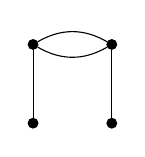
\begin{tikzpicture}[baseline={(current bounding box.center)}]
			\graph[no placement, nodes={circle, draw, fill=black, inner sep=0.2pt}]{
				d/$.$[at={(0,-1)}] -- a/$.$[at={(0,0)}] --[bend left] b/$.$[at={(1,0)}] -- c/$.$[at={(1,-1)}];
				a --[bend right] b;
			};
		\end{tikzpicture} \hspace{1cm}
		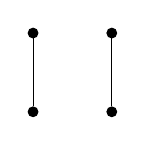
\begin{tikzpicture}[baseline={(current bounding box.center)}]
			\graph[no placement, nodes={circle, draw, fill=black, inner sep=0.2pt}]{
				a/$.$[at={(0,0)}] -- b/$.$[at={(0,-1)}];
				c/$.$[at={(1,0)}] -- d/$.$[at={(1,-1)}];
			};
		\end{tikzpicture} \hspace{1cm}
		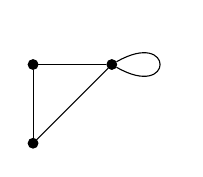
\begin{tikzpicture}[baseline={(current bounding box.center)}]
			\graph[no placement, nodes={circle, draw, fill=black, inner sep=0.2pt}]{
				a/$.$[at={(0,0)}] -- b/$.$[at={(1,0)}] --[out=-30, in=30, looseness=32] b -- c/$.$[at={(0,-1)}] -- a;
			};
		\end{tikzpicture}
	\end{center}
	From left to right:
	\begin{enumerate}
		\item Simple
		\item Not simple (has a loop)
		\item Simple
		\item Not simple (has a loop)
	\end{enumerate}
}

\dfn{Incident, Adjacent, Isloated}{
	\Defin{Incident Edges} An edge and a vertex are incident if and only if the vertex is an endpoint of the edge. \\
	\Defin{Adjacent Edges} Two edges are are adjacent if and only if they are incident with the same vertex. \\
	\Defin{Adjacent Vertices} Two vertices are adjacent if and only if their exists an edge such that both vertices are incident with it (they are connected by an edge). \\
	\Defin{Isolated Vertex} An isolated vertex is a vertex which is incident with no edges. \\
	}

\ex{}{
	$G$:
	\begin{center}
		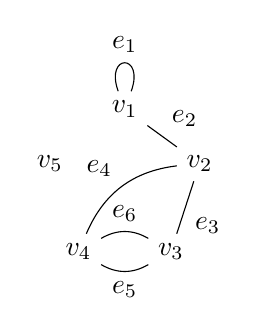
\begin{tikzpicture}[baseline={(current bounding box.center)}]
			\graph[multi, clockwise=5]{
				v1/$v_1$ --["$e_1$" above, out=70, in=110, looseness=8] v1;
				v2/$v_2$ --[draw=none] v2;
				v3/$v_3$ --[draw=none] v3;
				v4/$v_4$ --[draw=none] v4;
				v5/$v_5$ --[draw=none] v5;

				v1 --["$e_2$"] v2 --["$e_3$"] v3 --["$e_5$", bend left] v4;
				v4 --["$e_4$", bend left] v2;
				v4 --["$e_6$" above, bend left] v3;
			};
		\end{tikzpicture}
	\end{center}
	In the example above, 
	\begin{itemize}
		\item $e_3$ is incident with $v_2$ and $v_4$.
		\item $v_1$ is incident with $e_1$ and $e_2$.
		\item $e_2$ is adjacent to $e_3$ ($v_2$ in common).
		\item $v_2$ and $v_4$ are adjacent ($e_4$ in common).
		\item $v_1$ and $v_4$ are non-adjacent (no edges in common).
		\item $v_5$ is isolated (no incident edges).
	\end{itemize}
}

\dfn{Vertex Degree}{
	The degree of a vertex $v$ is the number of edges incident with $v$, where we count each loop twice. We denote this $\deg(v)$.
}

\ex{}{
	\begin{center}
		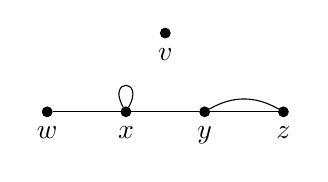
\begin{tikzpicture}
			\graph[no placement, nodes={circle, draw, fill=black, inner sep=0.2pt}]{
				w/$.$[at={(0,0)}] -- x/$.$[at={(1,0)}] -- y/$.$[at={(2,0)}] -- z/$.$[at={(3,0)}];
				v/$.$[at={(1.5,1)}];
				
				v [label=below:$v$];
				w [label=below:$w$];
				x [label=below:$x$];
				y [label=below:$y$];
				z [label=below:$z$];

				x --[out=120, in=60, looseness=16] x;
				y --[bend left] z;
			};
		\end{tikzpicture} \hspace{1cm}
		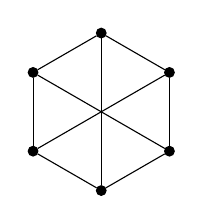
\begin{tikzpicture}%[baseline={(current bounding box.center)}]
			\graph[multi, clockwise=6, nodes={circle, draw, fill=black, inner sep=0.2pt}]{
				v1/$.$ --[draw=none] v1;
				v2/$.$ --[draw=none] v2;
				v3/$.$ --[draw=none] v3;
				v4/$.$ --[draw=none] v4;
				v5/$.$ --[draw=none] v5;
				v6/$.$ --[draw=none] v6;

				v1 -- v2 -- v3 -- v4 -- v5 -- v6 -- v1;
				v1 -- v4;
				v2 -- v5;
				v3 -- v6;
			};
		\end{tikzpicture}
	\end{center}

	With the graph on the left, $G$,
	\begin{itemize}
		\item $\deg(v) = 0$
		\item $\deg(w) = 1$
		\item $\deg(x) = 4$
		\item $\deg(y) = 3$
		\item $\deg(z) = 2$
	\end{itemize}
	The degree sum of $G$ is 10, which we note is $2\cd 5$, where 5 is interestingly the number of edges. \\

	With the graph on the right, $H$, each vertex has $\deg(v)=3$. There are 6 vertices, so the degree sum for $H$ is $3\cd6$. This is also $2\cd9$ and $H$ has 9 edges.
}

\thm{The Handshake Theorem}{
	Let $G$ be a graph with $n$ vertices,
	$$
		V(G) = \braces{v_1, v_2,\dots,v_n}.
	$$
	Then
	$$
		\sum_{i=1}^{n}\deg(v_i) = \deg(v_1)+\deg(v_2)+\dots+\deg(v_n) = 2\cd\abs{E(G)}.
	$$
	\Proof Let $G$ be a graph with $n$ vertices and $n\geq 1$ and $V(G)=\braces{v_1,v_2,\dots,v_n}$. \\
	First, the degree sum is can be counted by counting the degree of each vertex individually, then summing them, $\sum_{i=1}^{n} \deg(v_i)$. \\
	Second, let $e$ be any edge of $G$ with endpoints $\braces{v_i, v_j}$. Then, $e$ contributes 1 to the degree of $v_i$ and 1 to the degree of $v_j$. If $v_i=v_j$, then it still contributes 1 to $v_i$ and 1 to $v_j$ (which essentially means loops contributes 2 to a vertex). Hence, the degree sum is $2\abs{E(G)}$.\\
	$\tf\sum_{i=1}^{n} \deg(v_i) = 2\abs{E(G)}. \QED$
}

\cor{}{In any graph, there is an even number of vertices with odd degree.}

\subsection*{Walks, Trails, and Circuits}
\dfn{Walk}{
	Let $G$ be a graph, and let $v,w$ be vertices of $G$. A walk from $v$ to $w$ is a finite alternating sequence
	$$
		v_0e_1v_1e_2\dots v_{n-1}e_nv_n
	$$
	where $v_0=v$ and $v_n=w$ and $e_i$ is an edge with endpoints $\braces{v_{i-1},v_i}$, for $i\in\braces{1,2,\dots,n}$.
}

\ex{}{
	$G$:
	\begin{center}
		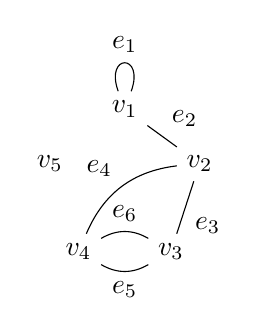
\begin{tikzpicture}[baseline={(current bounding box.center)}]
			\graph[multi, clockwise=5]{
				v1/$v_1$ --["$e_1$" above, out=70, in=110, looseness=8] v1;
				v2/$v_2$ --[draw=none] v2;
				v3/$v_3$ --[draw=none] v3;
				v4/$v_4$ --[draw=none] v4;
				v5/$v_5$ --[draw=none] v5;

				v1 --["$e_2$"] v2 --["$e_3$"] v3 --["$e_5$", bend left] v4;
				v4 --["$e_4$", bend left] v2;
				v4 --["$e_6$" above, bend left] v3;
			};
		\end{tikzpicture}
	\end{center}
	A path from $v_4$ to $v_3$ could be $v_4e_4v_2e_2v_1e_1v_1e_2v_2e_3v_3$. \\
	Another path could be $v_4e_6v_3$.
}

\dfn{Connected Graph}{
	A graph is connected if, given any two vertices, $v$ and $w$ in $G$, there exists a walk from $v$ to $w$.
}

\ex{}{
	\begin{center}
		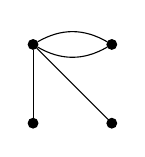
\begin{tikzpicture}[baseline={(current bounding box.center)}]
			\graph[multi, no placement, nodes={circle, draw, fill=black, inner sep=0.2pt}]{
				a/$.$[at={(0,0)}] --[bend left] b/$.$[at={(1,0)}] --[bend left] a;
				a -- c/$.$[at={(1,-1)}];
				a -- d/$.$[at={(0,-1)}];
			};
		\end{tikzpicture} \hspace{1cm}
		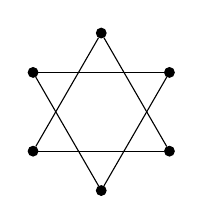
\begin{tikzpicture}[baseline={(current bounding box.center)}]
			\graph[multi, clockwise=6, nodes={circle, draw, fill=black, inner sep=0.2pt}]{
				v1/$.$ --[draw=none] v1;
				v2/$.$ --[draw=none] v2;
				v3/$.$ --[draw=none] v3;
				v4/$.$ --[draw=none] v4;
				v5/$.$ --[draw=none] v5;
				v6/$.$ --[draw=none] v6;

				v1 -- v3 -- v5 -- v1;
				v6 -- v2 -- v4 -- v6;
			};
		\end{tikzpicture}
	\end{center}
	The graph on the left is connected.\\
	The graph on the right is not connected.
}

\dfn{Trail and Circuit}{
	A trial is a walk whose edges are distinct. \\

	A circuit is a trial that starts and ends at the same vertex.
}

\dfn{Euler Circuit}{
	Let $G$ be a graph. An Euler circuit for $G$ is a circuit which uses every edge of $G$ exactly once.
}

\ex{}{
	\begin{center}
		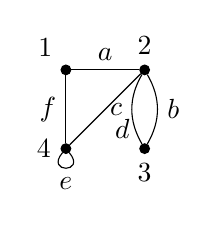
\begin{tikzpicture}[baseline={(current bounding box.center)}]
			\graph[multi, no placement, nodes={circle, draw, fill=black, inner sep=0.2pt}]{
				1/$.$[at={(0,0)}];
				2/$.$[at={(1,0)}];
				3/$.$[at={(1,-1)}];
				4/$.$[at={(0,-1)}];

				1[label=above left:1] --["$a$"] 2[label=above:2] --["$b$", bend left] 3[label=below:3] --["$c$", bend left] 2 --["$d$"] 4[label=left:4] --["$e$", in=230,out=310,looseness=10] 4 --["$f$"] 1;
			};
		\end{tikzpicture}
	\end{center}
	$3d2c4e4f1a2b3$ is a an Euler circuit.
}

\mlenma{}{
	If a graph $G$ has an Euler circuit, then each of its vertices has even degree.
}
\begin{proof}
	Let $G$ be a graph with an Euler circuit. Let $v\in V(G)$ be any vertex. We consider cases depending on whether or not $v$ is the start/end point of the Euler circuit. \\

	If $v$ is not the start/end point, then each time the Euler circuit vists passes through $v$, it comes along one edge, and out along another. Each pass contributes 2 to the degree of the the vertex. Hence $\deg(v)=2k,\ k\in\bbz_+$. \\

	If the $v$ is the start/end point, then the Euler circuit starts by exiting the vertex, contributing 1 to its degree. Then the circuit may pass through the vertex many times, but each time it enters, it leaves, contributing 2 to the degree for each pass through. Finally, the Euler circuit concludes at $v$, contributing another 1 to the degree. Hence, $\deg(V)=1+2k+1=2+2k=2(k+1),\ k\in\bbz_+$. \\

	Therefore, if $G$ has an Euler circuit, then each of its vertices has even degree.
\end{proof}

\thm{Euler Circuit}{
	Let $G$ be a connected graph. Then, $G$ has an Euler circuit if and only if every vertex of $G$ has even degree.
}

To find an Euler circuit, we can find any circuit in a graph, remove the circuit's edges, and then remove any isolated vertices. We can keep decomposing the graph in this way, until we find a trivial Euler circuit (a single vertex). Then we can ``splice'' together this decompositions, by 
\begin{center}
	\begin{tikzpicture}
		\graph[multi, no placement]{
			a[at={(-1,1)}, opacity=0] ->[blue] v/$.$[at={(0,0)}, circle, fill=black, inner sep=0.2pt] ->[blue] b[at={(-1,-1)}, opacity=0];
			c[at={(1,1)}, opacity=0] ->[red] v ->[red] d[at={(1,-1)}, opacity=0];
		};
	\end{tikzpicture}
\end{center}
entering a vertex which the two decomposed circuits have in common and exiting using the other circuit. In the example above, the blue and red edges represent different decomposed circuits. To create an Euler circut, we can enter with the blue, exit with the red, complete the red circuit, re-enter with the red, and exit with the blue, finally complete the blue circuit which can potentially complete an Euler circuit.

\ex{}{
	Decompose this graph, and find an Euler circuit.
	\begin{center}
		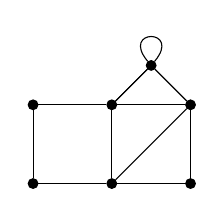
\begin{tikzpicture}[baseline={(current bounding box.center)}]
			\graph[multi, no placement, nodes={circle, draw, fill=black, inner sep=0.2pt}]{
				a/$.$[at={(0,0)}] -- b/$.$[at={(1,0)}] -- c/$.$[at={(1,-1)}] -- d/$.$[at={(0,-1)}] -- e/$.$[at={(-1,-1)}] -- f/$.$[at={(-1,0)}] -- a -- g/$.$[at={(0.5,0.5)}] -- b -- d -- a -- g --[in=50, out=130, looseness=16] g;
			};
		\end{tikzpicture} \\

		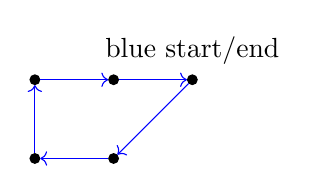
\begin{tikzpicture}[baseline={(current bounding box.center)}]
			\graph[multi, no placement, nodes={circle, draw, fill=black, inner sep=0.2pt}]{
				a/$.$[at={(0,0)}] ->[blue] b/$.$[at={(1,0)}] ->[blue] d/$.$[at={(0,-1)}] ->[blue] e/$.$[at={(-1,-1)}] ->[blue] f/$.$[at={(-1,0)}] ->[blue] a;

				b[label=above:blue start/end];
			};
		\end{tikzpicture}
		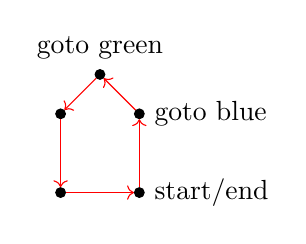
\begin{tikzpicture}[baseline={(current bounding box.center)}]
			\graph[multi, no placement, nodes={circle, draw, fill=black, inner sep=0.2pt}]{
				a/$.$[at={(0,0)}] <-[red] g/$.$[at={(0.5,0.5)}] <-[red] b/$.$[at={(1,0)}] <-[red] c/$.$[at={(1,-1)}] <-[red] d/$.$[at={(0,-1)}] <-[red] a;

				c[label=right:start/end];
				b[label=right:goto blue];
				g[label=above:goto green];
			};
		\end{tikzpicture}
		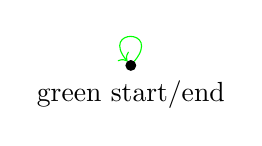
\begin{tikzpicture}[baseline={(current bounding box.center)}]
			\graph[multi, no placement, nodes={circle, draw, fill=black, inner sep=0.2pt}]{
				g/$.$[at={(0.5,0.5)}] ->[green, in=130, out=50, looseness=16] g;

				g[label=below:green start/end];
			};
		\end{tikzpicture}
	\end{center}
	I've decomposed the graph, and used the decomposition to find an Euler circuit, as required.
}

\dfn{Euler Trial}{
	Let $G$ be a graph and let $u,v\in V(G)$. An Euler trail is a trail from $u$ to $v$ that uses every edge exactly once.
}
\thm{Euler Trial}{
	Let $G$ be a connected graph and let $u,v\in V(G)$. \vspace{3pt}

	If $u=v$, then $G$ has an Euler trail from $u$ to $v$ if and only if every vertex of $G$ has even degree. \vspace{3pt}

	If $u\neq v$, then $G$ has an Euler trail from $u$ to $v$ if and only if $u,v$ have odd degree and all other vertices have even degree.
}

\section{Lecture 36}
\subsection*{Matrix Representations of Graphs}
\Defin{$m{\times}n$-matrix} An $m$-by-$n$ matrix over a set $S$ is a rectangular array of elements of $S$ arranged into $m$ rows and $n$ columns.
$$
	A = \begin{pmatrix}
		a_{11} 	& a_{12} & \dots & a_{1j} & \dots & a_{1n} \\
		a_{21} 	& a_{22} & \dots & a_{2j} & \dots & a_{2n} \\
		\vdots	& \vdots & \ddots& \cdots & \cdots & \vdots \\
		a_{i1} & a_{i2} & \dots & a_{ij} & \dots & a_{in} \\
		\vdots	& \vdots & \ddots& \cdots & \cdots & \vdots \\
		a_{m1} & a_{m2} & \dots & a_{mj} & \dots & a_{mn} 
	\end{pmatrix}
$$
We write $A=\sqbracks{a_{ij}}$ or $A=\sqbracks{a_{ij}}_{m{\times}n}$. The symbol $a_{ij}$ denotes the entry in row $i$, column $j$. \\
For our purposes, $S=\bbz_{\geq0}$.

\dfn{Adjacency Matrix}{
	Let $G$ be a graph with $n$ vertices and suppose we label the vertices $V(G)=\braces{v_1,v_2,\dots,v_n}$. \\

	The adjacency matrix of $G$ is the $n{\times}n,\ A=\sqbracks{a_{ij}}$, where $a_{ij}$ is the number of edges with the endpoints $\braces{v_i, v_j}$. ie,
	$$
		a_{ij} = \left\lbrace \begin{array}{ll} r & \text{if}\ \exists r\ \text{edges connecting } v_i \text{ and } v_j \\ 0 & \text{otherwise} \end{array} \right.
	$$
}

\ex{}{
	Write the adjacency matrix for the following graph:
	\begin{center}
		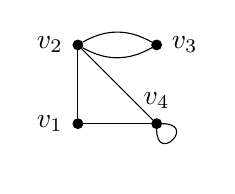
\begin{tikzpicture}
			\graph[multi, no placement, nodes={circle, draw, fill=black, inner sep=0.2pt}]{
				v2/$.$[at={(0,0)}] --[bend left] v3/$.$[at={(1,0)}] --[bend left] v2 -- v1/$.$[at={(0,-1)}] -- v4/$.$[at={(1,-1)}] --[out=270, in=0, looseness=12] v4 -- v2;

				v1[label=left:$v_1$];
				v2[label=left:$v_2$];
				v3[label=right:$v_3$];
				v4[label=above:$v_4$];
			};
		\end{tikzpicture}
	\end{center}
	$$
		A = \kbordermatrix{
					& v_1 & v_2 & v_3 & v_4\\
			v_1 & 0 	& 1 	& 0 	& 1	 \\
			v_2 & 1 	& 0 	& 2 	& 1	 \\
			v_3 & 0 	& 2 	& 0 	& 0	 \\
			v_4 & 1 	& 1 	& 0 	& 1	
		}
	$$
}
\nt{
	For an adjacency matrix $A=\sqbracks{a_ij},\ a_{ij}=a_{ji},\ \forall i,j\in\braces{1,2,\dots,n}$.
}

\dfn{Incidence Matrix}{
	Let $G$ be a graph with $n$ vertices and $m$ edges, and suppose we label the vertices $V(G)=\braces{v_1,v_2,\dots,v_n}$ and label the edges $E(G)=\braces{e_1,e_2,\dots,e_n}$. \\

	The incidence matrix for the graph $G$ is the $n{\times}m$ matrix $N=\sqbracks{a_{ij}}$ where each entry $n_{ij}$ is the number of times vertex $v_i$ is incident with $e_j$. ie,
	$$
		n_{ij} = \left\lbrace \begin{array}{ll} 2 & \text{if}\ e_j \text{ is a loop on vertex } v_i \\ 1 & \text{ if}\ e_j \text{ is an edge connecting } v_i \text{ to some other vertex} \\ 0 & \text{otherwise} \end{array} \right.
	$$
}

\ex{}{
	Write the incidence matrix for the following graph:
	\begin{center}
		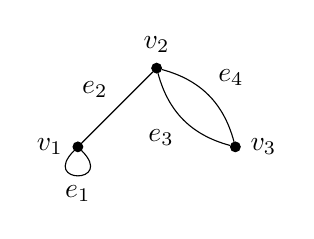
\begin{tikzpicture}
			\graph[multi, no placement, nodes={circle, draw, fill=black, inner sep=0.2pt}]{
				v2/$.$[at={(0,0)}] --["$e_4$", bend left] v3/$.$[at={(1,-1)}] --["$e_3$", bend left] v2 --["$e_2$" above left] v1/$.$[at={(-1,-1)}] --["$e_1$", out=315, in=225, looseness=16] v1;

				v1[label=left:$v_1$];
				v2[label=above:$v_2$];
				v3[label=right:$v_3$];
			};
		\end{tikzpicture}
	\end{center}
	$$
		A = \kbordermatrix{
					& e_1 & e_2 & e_3 & e_4\\
			v_1 & 2 	& 1 	& 0 	& 0	 \\
			v_2 & 0 	& 1 	& 1 	& 1	 \\
			v_3 & 0 	& 0 	& 1 	& 1	
		}
	$$
}
\nt{
	For every adjacency matrix, every column will contain two 1s or one 2. The sum of each row is the degree of the corresponding vertex.
}

\ex{}{
	Draw the graphs corresponding to the following matricies:
	$$
		A(G) = \kbordermatrix{
					& v_1	& v_2	& v_3	& v_4 \\
			v_1	& 0		& 1		& 1		& 0		\\
			v_2	& 1		& 1		& 0		& 0		\\
			v_3	& 1		& 0		& 0		& 2		\\
			v_4	& 0		& 0		& 2		& 0
		}\qquad
		N(H) = \kbordermatrix{
					& e_1	& e_2	& e_3	& e_4	& e_5 \\
			v_1	& 1		& 0		& 1		& 0		& 0		\\
			v_2	& 1		& 2		& 0		& 0		& 0		\\
			v_3	& 0		& 0		& 1		& 1		& 1		\\
			v_4	& 0		& 0		& 0		& 1		& 1		\\
		}
	$$
	\begin{center}
		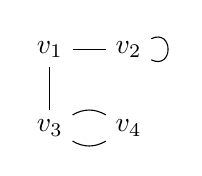
\begin{tikzpicture}[baseline={(current bounding box.center)}]
			\graph[multi, no placement]{
				v1/$v_1$[at={(0,0)}];
				v2/$v_2$[at={(1,0)}];
				v3/$v_3$[at={(0,-1)}];
				v4/$v_4$[at={(1,-1)}];

				v1 -- v2;
				v1 -- v3;
				v2 --[out=-25, in=25, looseness=3] v2;
				v3 --[bend left] v4;
				v3 --[bend right] v4;
			};
		\end{tikzpicture}\hspace{4cm}
		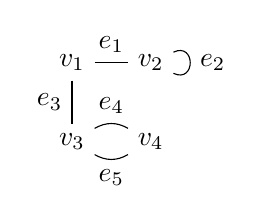
\begin{tikzpicture}[baseline={(current bounding box.center)}]
			\graph[multi, no placement]{
				v1/$v_1$[at={(0,0)}];
				v2/$v_2$[at={(1,0)}];
				v3/$v_3$[at={(0,-1)}];
				v4/$v_4$[at={(1,-1)}];

				v1 --["$e_1$"] v2;
				v2 --["$e_2$" right, out=-25, in=25, looseness=3] v2;
				v1 --["$e_3$" left] v3;
				v3 --["$e_4$", bend left] v4;
				v3 --["$e_5$" below, bend right] v4;
			};
		\end{tikzpicture}
	\end{center}
}

\subsection*{Trees}
\dfn{Tree}{
	\Defin{Circuit-Free Graph} A graph is circuit-free if and only if it has no nontrivial circuits. \\

	A graph is a tree if and only if it is connected and circuit-free. \\

	Since loops and multiple edges are nontrivial circuits, trees are simple graphs.
}

\ex{}{
	\begin{center}
		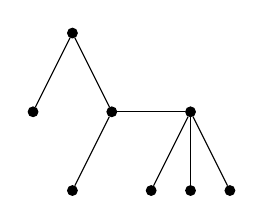
\begin{tikzpicture}[baseline={(current bounding box.center)}]
			\graph[simple, no placement, nodes={circle, draw, fill=black, inner sep=0.2pt}]{
				a/$.$[at={(0,0)}] -- b/$.$[at={(-0.5,-1)}];
				a -- c/$.$[at={(0.5,-1)}] -- d/$.$[at={(0,-2)}];
				c -- e/$.$[at={(1.5,-1)}] -- f/$.$[at={(1,-2)}];
				e -- g/$.$[at={(1.5,-2)}];
				e -- h/$.$[at={(2,-2)}];
			};
		\end{tikzpicture} \hspace{1cm}
		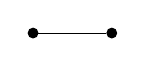
\begin{tikzpicture}[baseline={(current bounding box.center)}]
			\graph[simple, no placement, nodes={circle, draw, fill=black, inner sep=0.2pt}]{
				a/$.$[at={(0,0)}] -- b/$.$[at={(1,0)}];
			};
		\end{tikzpicture} \hspace{1cm}
		
\begin{tikzpicture}[baseline={(current bounding box.center)}]
			\graph[simple, no placement, nodes={circle, draw, fill=black, inner sep=0.2pt}]{
				a/$.$[at={(0,0)}];
			};
		\end{tikzpicture} 
	\end{center}
	All three of these are examples of trees.
}

\thm{Trees are\dots}{
	A graph, $G$ with $n$ vertices, is a tree if and only if $G$ is simple, connected, and has $n-1$ edges.
}

\end{document}
